% !TeX spellcheck = sl_SI
% vim: set spell spelllang=sl:
% za preverjanje črkovanja, če se uporablja Texstudio ali vim
\documentclass[12pt,a4paper,twoside]{article}
\usepackage[utf8]{inputenc}  % pravilno razpoznavanje unicode znakov

% NASLEDNJE UKAZE USTREZNO POPRAVI
\newcommand{\program}{Pedagoška matematika} % ime studijskega programa
\newcommand{\imeavtorja}{Simon Besednjak} % ime avtorja
\newcommand{\imementorja}{prof.~dr.~Marjetka Knez} % akademski naziv in ime mentorja, uporabi poln naziv, prof.~dr.~, doc.~dr., ali izr.~prof.~dr.
\newcommand{\imesomentorja}{} % akademski naziv in ime somentorja, če ga imate
\newcommand{\naslovdela}{Dvojne PH krivulje}
\newcommand{\letnica}{2021} % letnica magistriranja
\newcommand{\opis}{Delo obravnava lastnosti krivulj z pitagorejskih hodografom.}  % Opis dela v eni povedi. Ne sme vsebovati matematičnih simbolov v $ $.
\newcommand{\kljucnebesede}{PH krivulje\sep dvojne PH krivulje} % ključne besede, ločene z \sep, da se PDF metapodatki prav procesirajo
\newcommand{\keywords}{PH curves\sep double PH curves} % ključne besede v angleščini
\newcommand{\organization}{Univerza v Ljubljani, Fakulteta za matematiko in fiziko} % fakulteta
\newcommand{\literatura}{literatura}  % pot do datoteke z literaturo (brez .bib končnice)
\newcommand{\sep}{, }  % separator med ključnimi besedami v besedilu
% KONEC PODATKOV

\usepackage{bibentry}         % za navajanje literature v programu dela s celim imenom
\nobibliography{\literatura}
\newcommand{\plancite}[1]{\item[\cite{#1}] \bibentry{#1}} % citiranje v programu dela

\usepackage{filecontents}  % za pisanje datoteke s PDF metapodatki
\usepackage{silence} \WarningFilter{latex}{Overwriting file}  % odstrani annoying warning o obstoju datoteke
% datoteka s PDF metapodatki, zgenerira se kot magisterij.xmpdata
\begin{filecontents*}{\jobname.xmpdata}
  \Title{\naslovdela}
  \Author{\imeavtorja}
  \Keywords{\kljucnebesede}
  \Subject{matematika}
  \Org{\organization}
\end{filecontents*}

\usepackage[a-1b]{pdfx}  % zgenerira PDF v tem PDF/A-1b formatu, kot zahteva knjižnica
\hypersetup{bookmarksopen, bookmarksdepth=3, colorlinks=true,
  linkcolor=black, anchorcolor=black, citecolor=black, filecolor=black,
  menucolor=black, runcolor=black, urlcolor=black, pdfencoding=auto,
  breaklinks=true, psdextra}

\usepackage[slovene]{babel}  % slovenščina
\usepackage[T1]{fontenc}     % naprednejše kodiranje fonta
\usepackage{amsmath,amssymb,amsfonts,amsthm} % matematični paketi
\usepackage{graphicx}     % za slike
\usepackage{emptypage}    % prazne strani so neoštevilčene, ampak so štete
\usepackage{units}        % fizikalne enote kot \unit[12]{kg} s polovico nedeljivega presledka, glej primer v kodi
\usepackage{makeidx}      % za stvarno kazalo, lahko zakomentiraš, če ne rabiš
\makeindex                % za stvarno kazalo, lahko zakomentiraš, če ne rabiš
% oblika strani
\usepackage[
  top=3cm,
  bottom=3cm,
  inner=3.5cm,      % margini za dvostransko tiskanje
  outer=2.5cm,
  footskip=40pt     % pozicija številke strani
]{geometry}

% VEČ ZANIMIVIH PAKETOV
% \usepackage{array}      % več možnosti za tabele
% \usepackage[list=true,listformat=simple]{subcaption}  % več kot ena slika na figure, omogoči slika 1a, slika 1b
% \usepackage[all]{xy}    % diagrami
% \usepackage{doi}        % za clickable DOI entrye v bibliografiji
% \usepackage{enumerate}     % več možnosti za sezname

% Za barvanje source kode
% \usepackage{minted}
% \renewcommand\listingscaption{Program}

% Za pisanje psevdokode
% \usepackage{algpseudocode}  % za psevdokodo
% \usepackage{algorithm}
% \floatname{algorithm}{Algoritem}
% \renewcommand{\listalgorithmname}{Kazalo algoritmov}

% DRUGI TVOJI PAKETI:
% tukaj
\newcommand{\iu}{\mathrm{i}\mkern1mu} % za imaginarno enoto
%\allowdisplaybreaks

\setlength{\overfullrule}{50pt} % označi predlogo vrstico
\pagestyle{plain}               % samo številka strani na dnu, nobene glave / noge

% ukazi za matematična okolja
\theoremstyle{definition} % tekst napisan pokončno
\newtheorem{definicija}{Definicija}[section]
%\newtheorem{primer}[definicija]{Primer}
\newtheorem{opomba}[definicija]{Opomba}
\newtheorem{aksiom}{Aksiom}

\theoremstyle{plain} % tekst napisan poševno
\newtheorem{lema}[definicija]{Lema}
\newtheorem{izrek}[definicija]{Izrek}
\newtheorem{trditev}[definicija]{Trditev}
\newtheorem{posledica}[definicija]{Posledica}

\newtheoremstyle{primerstyle}% name of the style to be used
  {}% measure of space to leave above the theorem. E.g.: 3pt
  {}% measure of space to leave below the theorem. E.g.: 3pt
  {}% name of font to use in the body of the theorem
  {0pt}% measure of space to indent
  {\bfseries}% name of head font
  {}% punctuation between head and body
  {0pt}% space after theorem head; " " = normal interword space
  {\thmname{#1}\thmnumber{ #2}\textnormal{\thmnote{ (#3)}}}
  
\theoremstyle{primerstyle}
\newtheorem{primer}[definicija]{Primer}

\numberwithin{equation}{section}  % števec za enačbe zgleda kot (2.7) in se resetira v vsakem poglavju

% Matematični ukazi
\newcommand{\R}{\mathbb R}
\newcommand{\N}{\mathbb N}
\newcommand{\Z}{\mathbb Z}
\renewcommand{\C}{\mathbb C}
\newcommand{\Q}{\mathbb Q}
\newcommand{\quat}{\mathbb H}
\newcommand{\tangenta}{\frac{\mathbf{r}'}{\lVert \mathbf{r}'\rVert}}
\newcommand{\normala}{\frac{\mathbf{r}'\times\mathbf{r}''}{\lVert \mathbf{r}'\times\mathbf{r}'' \rVert}\times \mathbf{t}}
\newcommand{\binormala}{\frac{\mathbf{r}'\times\mathbf{r}''}{\lVert \mathbf{r}'\times\mathbf{r}'' \rVert}}
\newcommand{\fleksija}{\frac{\lVert \mathbf{r}'\times\mathbf{r}'' \rVert}{\sigma^3}}
\newcommand{\torzija}{\frac{(\mathbf{r}'\times\mathbf{r}'')\cdot\mathbf{r}'''}{\lVert \mathbf{r}'\times\mathbf{r}'' \rVert^2}}
\newcommand{\tV}{\mathbf{t}}
\newcommand{\aV}{\mathbf{a}}
\newcommand{\bV}{\mathbf{b}}
\newcommand{\cV}{\mathbf{c}}
\newcommand{\eV}{\mathbf{e}}
\newcommand{\fV}{\mathbf{f}}
\newcommand{\hV}{\mathbf{h}}
\newcommand{\nV}{\mathbf{n}}
\newcommand{\pV}{\mathbf{p}}
\newcommand{\qV}{\mathbf{q}}
\newcommand{\rV}{\mathbf{r}}
\newcommand{\iV}{\mathbf{i}}
\newcommand{\jV}{\mathbf{j}}
\newcommand{\kV}{\mathbf{k}}
\newcommand{\vV}{\mathbf{v}}
\newcommand{\wV}{\mathbf{w}}
\newcommand{\zV}{\mathbf{z}}
\newcommand{\ndr}{\lVert \mathbf{r}'\rVert} % norma prvega odvoda
\newcommand{\ndrtddr}{\lVert \mathbf{r}'\times \mathbf{r}'' \rVert} % norma vektorskega produkta prvega in drugega odvoda
\newcommand{\AQ}{\mathcal{A}}
\newcommand{\BQ}{\mathcal{B}}
\newcommand{\CQ}{\mathcal{C}}
\newcommand{\DQ}{\mathcal{D}}
\newcommand{\QQ}{\mathcal{Q}}
\newcommand{\VQ}{\mathcal{V}}
\newcommand{\UQ}{\mathcal{U}}
\newcommand{\balpha}{\boldsymbol \alpha}
\newcommand{\bbeta}{\boldsymbol \beta}
\newcommand{\bgamma}{\boldsymbol \gamma}
\newcommand{\bdelta}{\boldsymbol \delta}
\newcommand{\brho}{\boldsymbol \rho}
\newcommand{\btau}{\boldsymbol \tau}
\newcommand{\btalpha}{\tilde{\boldsymbol \alpha}}
\newcommand{\btbeta}{\tilde{\boldsymbol \beta}}
\newcommand{\bell}{\boldsymbol \ell}
\newcommand{\dFrac}[2][t]{\frac{\mathrm{d}#2}{\mathrm{d}#1}} %odvod, default spremenljivka je t

% \DeclareMathOperator{\tr}{tr}  % morda potrebuješ operator za sled ali kaj drugega?
\DeclareMathOperator{\st}{st}
\DeclareMathOperator{\hopf}{H}
\DeclareMathOperator{\ReC}{Re}
\DeclareMathOperator{\ImC}{Im}
\DeclareMathOperator{\nhopf}{\hat{H}}

% bold matematika znotraj \textbf{ }, tudi v naslovih, kot \omega spodaj
\makeatletter \g@addto@macro\bfseries{\boldmath} \makeatother

% Poimenuj kazalo slik kot ``Kazalo slik'' in ne ``Slike''
\addto\captionsslovene{
  \renewcommand{\listfigurename}{Kazalo slik}%
}

\usepackage{titlesec}
\titleformat*{\subsubsection}{\em} % da podpodpoglavja niso bold
%\titleformat*{\subsection}{\normalfont}

% če želiš, da se poglavja začnejo na lihih straneh zgoraj
% \let\oldsection\section
% \def\section{\cleardoublepage\oldsection}

% Pravilno deljenje besed
%\hyphenation{kro-žnic} 

%%%%%%%%%%%%%%%%%%%%%%%%%%%%%%%%%%%%%%%%%%
%%%%%%           DOCUMENT           %%%%%%
%%%%%%%%%%%%%%%%%%%%%%%%%%%%%%%%%%%%%%%%%%

\begin{document}

\pagenumbering{roman} % začnemo z rimskimi številkami
\thispagestyle{empty} % ampak na prvi strani ni številke

\noindent{\large
UNIVERZA V LJUBLJANI\\[1mm]
FAKULTETA ZA MATEMATIKO IN FIZIKO\\[5mm]
\program\ -- 2.~stopnja}
% ustrezno dopolni za IŠRM
\vfill

\begin{center}
  \large
  \imeavtorja\\[3mm]
  \Large
  \textbf{\MakeUppercase{\naslovdela}}\\[10mm]
  \large
  Magistrsko delo \\[1cm]
  Mentor: \imementorja \\[2mm] % ustrezno popravi spol
%   Somentor: \imesomentorja   % dodaj, če potrebno
\end{center}
\vfill

\noindent{\large Ljubljana, \letnica}

\cleardoublepage

%% sem pride IZJAVA O AVTORSTVU  -- SE NATISNE V VIS

% zahvala
\pdfbookmark[1]{Zahvala}{zahvala} %
\section*{Zahvala}
Neobvezno.
Zahvaljujem se \dots
% end zahvala -- izbriši vse med zahvala in end zahvala, če je ne rabiš

\cleardoublepage

\pdfbookmark[1]{\contentsname}{kazalo-vsebine}
\tableofcontents

% list of figures
 \cleardoublepage
 \pdfbookmark[1]{\listfigurename}{kazalo-slik}
 \listoffigures
% end list of figures

\cleardoublepage

\section*{Program dela}
\addcontentsline{toc}{section}{Program dela} % dodajmo v kazalo
Mentor naj napiše program dela skupaj z osnovno literaturo. Na literaturo se
lahko sklicuje kot~\cite{lebedev2009introduction}, \cite{gurtin1982introduction},
\cite{zienkiewicz2000finite}, \cite{STtemplate}.

\section*{Osnovna literatura}
Literatura mora biti tukaj posebej samostojno navedena (po pomembnosti) in ne
le citirana. V tem razdelku literature ne oštevilčimo po svoje, ampak uporabljamo
okolje itemize in ukaz plancite, saj je celotna literatura oštevilčena na koncu.
\begin{itemize}
  \plancite{DPHclanek1}
  \plancite{DPHclanek2}
  \plancite{farouki2008pythagorean}
\end{itemize}

\vspace{2cm}
\hspace*{\fill} Podpis mentorja: \phantom{prostor za podpis}

% \vspace{2cm}
% \hspace*{\fill} Podpis somentorja: \phantom{prostor za podpis}

\cleardoublepage
\pdfbookmark[1]{Povzetek}{abstract}

\begin{center}
\textbf{\naslovdela} \\[3mm]
\textsc{Povzetek} \\[2mm]
\end{center}
Tukaj napišemo povzetek vsebine. Sem sodi razlaga vsebine in ne opis tega, kako je delo
organizirano.

\vfill
\begin{center}
\textbf{English translation of the title} \\[3mm] % prevod slovenskega naslova dela
\textsc{Abstract}\\[2mm]
\end{center}

An abstract of the work is written here. This includes a short description of
the content and not the structure of your work.

\vfill\noindent
\textbf{Math.~Subj.~Class.~(2010):} oznake kot 74B05, 65N99, na voljo so na naslovu
\url{http://www.ams.org/msc/msc2010.html} \\[1mm]
\textbf{Ključne besede:} \kljucnebesede \\[1mm]
\textbf{Keywords:} \keywords

\cleardoublepage

\setcounter{page}{1}    % od sedaj naprej začni zopet z 1
\pagenumbering{arabic}  % in z arabskimi številkami

%%%%%%%%%%%%%%%%%%%%%%%%%%%%%%%%%%%%%%%%%%%%%%%%%%%%%%%%%%%%%%%%%%%%%
\section{Uvod}

Napišite kratek zgodovinski in matematični uvod.  Pojasnite motivacijo za problem, kje
nastopa, kje vse je bil obravnavan. Na koncu opišite tudi organizacijo dela -- kaj je v
katerem razdelku.
%%%%%%%%%%%%%%%%%%%%%%%%%%%%%%%%%%%%%%%%%%%%%%%%%%%%%%%%%%%%%%%%%%%%%
\section{Osnovni pojmi in uvodne definicije}

\subsection{Prostorske krivulje}
\subsubsection{Osnovne lastnosti}

Krivulje v prostoru si lahko predstavljamo kot tirnice, po katerih potuje točka v gibanju. Najlažje jih podamo
v parametrični obliki
\begin{equation*}
\rV:I \to \R^3, I \subseteq \R, \quad \rV(t)=(x(t),y(t),z(t)), \quad t \in I,
\end{equation*}
kjer so 
$x,\text{ } y \text{ in } z$ običajne skalarne funkcije parametra $t.$ Več različnih parametrizacij lahko opisuje
isto krivuljo. V nadaljevanju bomo predpostavili, da so $x$, $y$ in $z$ vsaj dvakrat zvezno odvedljive funkcije.
Odvod krivulje $\rV$ dobimo tako, da krivuljo odvajamo po komponentah:
$$\rV':I \to \R^3, \quad \rV'(t)=(x'(t),y'(t),z'(t)), \quad t \in I.$$
Vektorsko polje, ki ga pri tem dobimo, imenujemo tudi \textit{hodograf} krivulje $\rV.$ Več o parametrično podanih krivuljah si lahko bralec prebere v \cite{struik1961lectures}.

\subsubsection{Ločna dolžina in tangenta na krivuljo}

Pravimo, da je krivulja $\rV$ regularna, če je njen odvod $\rV'(t) \neq 0$ za vse vrednosti $t \in I.$ Od sedaj bomo privzeli, da je krivulja regularna. Odvod regularne krivulje pa lahko zapišemo tudi v malce drugačni obliki
\begin{equation}
	\label{eq2_1}
	\rV'(t)=\sigma(t)\tV(t),
\end{equation}
kjer je $\sigma(t)$ funkcija, ki slika z začetne domene $I$ v $\R,$
\begin{equation}
	\sigma(t)=\lVert \rV'(t)\rVert=\sqrt{x'^2(t)+y'^2(t)+z'^2(t)},
\end{equation}
in predstavlja spremembo ločne dolžine krivulje v odvisnosti od parametra $t,$ s $\tV(t)$ pa je označeno enotsko tangentsko vektorsko polje na krivuljo $\rV,$ izračunano pri parametru $t,$
\begin{equation}
	\label{enotski_tangentni_vektor}
	\tV(t)=\frac{\rV'(t)}{\lVert \rV'(t) \rVert}=
	\frac{\rV'(t)}{\sigma(t)}.
\end{equation}
S pomočjo funkcije $\sigma(t)$ lahko izrazimo tudi dolžino loka krivulje. Če je $I=[a,b],$ potem je ločna dolžina enaka
\begin{equation}
	\int_a^b\sqrt{x'^2(t)+y'^2(t)+z'^2(t)}dt=\int_a^b\lVert \rV'(t) \rVert dt =\int_a^b\sigma(t)dt.
\end{equation}

Na intervalu $I=[a,b]$ lahko dolžino loka od točke $a$ do $t$ izrazimo tudi kot funkcijo parametra $t:$
\begin{equation}
	\label{naravna_parametrizacija}
	s=s(t)=\int_a^t\sigma(\xi)d\xi.
\end{equation}
Če je krivulja $\rV$ regularna, je po osnovnem izreku analize funkcija \eqref{naravna_parametrizacija} zvezno odvedljiva, povsod različna od nič:
$$\frac{ds}{dt}=\sigma(t)=\lVert\rV'(t)\rVert.$$
Torej lahko vzamemo $s=s(t)$ kot nov parameter na $I.$ Taki parametrizaciji pravimo \emph{naravna parametrizacija} krivulje $\rV.$ Označimo $\brho(s)=\rV(t(s)).$ Izračunajmo odvod krivulje po parametru $s:$
$$\frac{d\brho}{ds}=\rV'(t(s))\frac{dt(s)}{ds}=\frac{\rV'(t(s))}{\frac{ds}{dt}}=\frac{\rV'(t(s))}{\lVert\rV'(t(s))\rVert}.$$
Dobili smo enotski tangenti vektor \eqref{enotski_tangentni_vektor}, kar pomeni, da je dolžina $\lVert\brho'(s)\rVert$ vedno enaka 1. Drugače povedano: parametrična hitrost pri naravni parametrizaciji je identično enaka 1. Več o naravni parametrizaciji si lahko bralec prebere v \cite[str. 51]{lipschutz1969schaum}.

\subsubsection{Ukrivljenost in Frenetovo ogrodje}

Sedaj bomo uvedli dve novi enotski vektorski polji, ki bosta skupaj z enotsko tangento v vsaki točki na krivulji tvorili ortonormalno bazo za prostor $\R^3.$ V nadaljevanju bomo ponekod v enačbah in izpeljavah zaradi preglednosti izpustili parameter $t.$

Ker je $\tV$ enotsko tangento polje, vedno velja $\tV \cdot \tV=\lVert \tV \rVert^2 =1.$ Če to enačbo odvajamo, dobimo, da je $\tV' \cdot \tV=0,$ kar pomeni, da je $\tV'$ pravokoten na $\tV$ pri vsakemu parametru $t.$ Torej lahko (implicitno) definiramo enotsko vektorsko polje $\pV$ na naslednji način: odvod enotske tangente je enak
\begin{equation}
	\label{eq2_5}
	\tV'(t)=\sigma(t)\kappa(t)\pV(t),
\end{equation}
kjer je $\kappa(t)$ nenegativna funkcija parametra $t.$ Tako ima vektorsko polje $\pV$ isto smer kot $\tV'.$ Prav tako je $\pV$ pravokoten na enotsko tangento $\tV.$ Da bi lahko $\pV$ eksplicitno izrazili, si s pomočjo enačbe \eqref{eq2_1} oglejmo drugi odvod krivulje $\rV:$
\begin{equation}
	\label{eq2_6}
	\rV''=\sigma'\tV+\sigma\tV'.
\end{equation}
Iz \eqref{eq2_1} in zgornje enačbe sledi naslednja enakost
\begin{equation}
	\label{eq2_7}
	\rV'(t) \times \rV''(t)=\sigma^3(t)\kappa(t)\tV(t) \times \pV(t).
\end{equation}
Ker je $\pV$ definirano kot enotsko vektorsko polje, ki je ortogonalno na $\tV,$ je potem
\begin{equation}
	\label{kappa1}
	\kappa(t)=\frac{\lVert \rV'(t) \times \rV''(t) \rVert}{\sigma^3(t)}=\frac{\lVert \rV'(t) \times \rV''(t) \rVert}{\lVert \rV'(t) \rVert^3}.
\end{equation}
To lahko naredimo, saj smo predpostavili, da je $\kappa(t)$ nenegativna funkcija. Sedaj si oglejmo, čemu je enaka naslednja količina:
\begin{align}
	\frac{\rV'\times \rV''}{\lVert \rV'\times \rV'' \rVert} \times \tV &= \frac{1}{\lVert \rV'\times \rV'' \rVert} \left ( \sigma^3 \frac{\lVert \rV'\times \rV'' \rVert}{\sigma^3}\tV \times \pV\right ) \times \tV \nonumber \\
	&= (\tV \times \pV) \times \tV \nonumber \\
	&= -(\tV \cdot \pV)\tV + (\tV \cdot \tV)\pV \label{normala} \\
	&= \pV. \nonumber
\end{align}
Količini $\pV$ pravimo \textit{normala} ali \textit{glavna normala} na krivuljo $\rV,$ količini $\kappa$ pa \textit{fleksijska ukrivljenost} krivulje $\rV.$ Enostavno se da preveriti, da je fleksijska ukrivljenost neodvisna od izbire parametrizacije krivulje.
Definirali smo že enotsko tangento in enotsko normalo. Najti moramo še eno enotsko vektorsko polje, ki je ortogonalno na obe prejšnji. To lahko naredimo direktno z vektorskim produktom
\begin{equation}
	\label{binormala}
	\bV=\tV \times \pV=\frac{\rV'\times \rV''}{\lVert \rV'\times \rV'' \rVert}.
\end{equation}
Tej količini pravimo \textit{binormala} krivulje $\rV.$ Vektorska polja $\tV,\mathbf{ p}, \mathbf{ b}$ na vsaki točki krivulje $\rV$ tvorijo ortonormirano bazo prostora $\R^3.$ To trojico imenujemo tudi \textit{Frenetovo ogrodje}. Če je binormala nek konstanten vektor za vsak parameter $t$ (z dolžino~1), sledi, da vektorski polji $\tV$ in $\pV$ ležita v isti ravnini, kar pomeni, da celotna krivulja $\rV$ leži v tej isti ravnini.

Recimo, da velja $\bV' \neq 0.$ To pomeni, da imamo res opravka s prostorsko krivuljo. Če odvajamo enačbo \eqref{binormala} in uporabimo \eqref{eq2_5}, dobimo, da je odvod binormale enak $\bV'=\tV \times \pV'.$ Ker ima za vsak parameter $t$ vektor $\pV$ dolžino 1, sta potem vektorski polji $\pV$ in $\pV'$ ortogonalni (to lahko takoj preverimo z odvajanjem skalarnega produkta vektorskega polja $\pV$ s samim seboj). Torej se da izraziti $\pV'$ z $\bV$ in $\tV,$ kar pa pomeni, da se da $\bV'$ izraziti z $\tV \times \bV:$
\begin{equation}
	\label{eq2_11}
	\bV'(t)=\sigma(t)\tau(t)\tV(t)\times \bV(t)=-\sigma(t)\tau(t)\pV(t).
\end{equation}
Funkciji $\tau(t)$ pravimo \textit{torzijska ukrivljenost} krivulje $\rV.$ Da se dokopljemo do njenega eksplicitnega zapisa, najprej preuredimo in odvajamo enačbo \eqref{eq2_7}:
\begin{align*}
	(\rV' \times \rV'')'&=(\sigma^3\kappa \bV)'\\
	\rV' \times \rV''' &= 3\sigma^2\sigma'\kappa\bV+\sigma^3\kappa'\bV+\sigma^3\kappa\bV'\\
	&=-\sigma^4\kappa\tau\pV+\sigma^2(3\sigma'\kappa+\sigma\kappa')\bV.
\end{align*}
V zadnjem koraku smo upoštevali vrednost količine $\bV'.$ Če vrednost $\rV'\times \rV'''$ skalarno pomnožimo z $\rV'',$ dobimo
\begin{equation}
	(\rV'\times\rV''')\cdot\rV''=-\sigma^6\kappa^2\tau.
\end{equation}
Pri tem smo upoštevali \eqref{eq2_6}, \eqref{eq2_5} in ortonormiranost Frenetovega ogrodja. Če zamenjamo vrstni red v mešanem produktu v zgornji enačbi in upoštevamo \eqref{kappa1}, vidimo, da je torzijska ukrivljenost enaka
\begin{equation}
	\label{tau1}
	\tau(t)=\frac{\big(\rV'(t)\times\rV''(t)\big)\cdot\rV'''(t)}{\lVert \rV'(t)\times \rV''(t) \rVert^2}.
\end{equation}
Vidimo torej, da je torzijska ukrivljenost krivulje neničelna natanko takrat, ko so $\rV', \text{ } \rV''$ in $\rV'''$ linearno neodvisni, kar je ravno takrat, ko je krivulja res prostorska.

Poskusimo sedaj izraziti še odvod glavne normale. Najprej iz formul \eqref{normala} in \eqref{binormala} opazimo, da velja $\pV=\bV\times\tV.$ Sedaj odvajamo
\begin{align*}
	\pV'&=(\bV\times\tV)'\\
	&=\bV'\times\tV+\bV\times\tV'\\
	&=(-\sigma\tau\pV)\times\tV+\bV\times(\sigma\kappa\pV)\\
	&=-\sigma\kappa\tV+\sigma\tau\bV.
\end{align*}
Pri računanju smo uporabili formuli \eqref{eq2_5} in \eqref{eq2_11} za odvod enotske tangente in odvod binormale. Vse te tri formule lahko kompaktneje zapišemo v matrični obliki
\begin{equation}
	\label{frenetove_formule}
	\begin{bmatrix}
		\tV'\\
		\pV'\\
		\bV'
	\end{bmatrix}=
	\sigma
	\begin{bmatrix}
		0&\kappa&0\\
		-\kappa&0&\tau\\
		0&-\tau&0
	\end{bmatrix}
	\begin{bmatrix}
		\tV\\
		\pV\\
		\bV
	\end{bmatrix}.
\end{equation}
Če je krivulja $\rV$ podana v naravni parametrizaciji, vemo, da je njena parametrična hitrost identično enaka 1: $\sigma\equiv 1.$ Zato se v naravni parametrizaciji te formule izražajo takole:
\begin{equation}
	\label{naravne_frenetove_formule}
	\begin{bmatrix}
		\tV'\\
		\pV'\\
		\bV'
	\end{bmatrix}=
	\begin{bmatrix}
		0&\kappa&0\\
		-\kappa&0&\tau\\
		0&-\tau&0
	\end{bmatrix}
	\begin{bmatrix}
		\tV\\
		\pV\\
		\bV
	\end{bmatrix}.
\end{equation}
Tem formulam pravimo tudi \emph{Frenetove formule.}

\subsection{Bézierjeve krivulje in Bernsteinovi polinomi}
\label{bern_poli_bez_kri_poglavje}
Polinomske in racionalne krivulje se v računalniško podprtem geometrijskem oblikovanju na široko uporabljajo, saj nam omogočajo učinkovitejše računanje. Eden izmed najpomembnejših tipov krivulj so Bézierjeve krivulje. Spomnili se bomo, kako pridemo do njih preko Bernsteinovih polinomov ter si ogledali nekaj lastnosti \cite{farin2002handbook}.

\emph{Splošna Bézierjeva krivulja stopnje} $n$ je oblike
\begin{equation}
	\label{splosna_bezier}
	\rV(t)=\sum_{i=0}^n\bV_iB_i^n(t)\quad t\in[0,1],
\end{equation}
kjer so
\begin{equation}
	\label{splosni_bernstein}
	B_i^n(t)=\binom{n}{i}(1-t)^{n-i}t^i
\end{equation}
\emph{Bernsteinovi polinomi stopnje} $n$ z binomskimi koeficienti
$$\binom{n}{i}=\frac{n!}{(n-i)!i!}\quad\text{za}\quad 0\leq i \leq n\quad\text{in}\quad\binom{n}{i}=0\quad\text{za}\quad i>n,$$
točke $\bV_i\in\R^3$ pa sestavljajo \emph{kontrolni poligon} Bézierjeve krivulje in jim zato rečemo tudi kontrolne točke.
\pagebreak

Naštejmo sedaj nekaj najpomembnejših lastnosti Bézierjevih krivulj:
\begin{itemize}
	\item Vsaka Bézierjeva krivulja interpolira začetno in končno kontrolno točko: $\rV(0)=\bV_0$ in $\rV(1)=\bV_n.$
	\item \emph{Simetričnost:} Kontrolni poligon $\bV_0,\dots,\bV_n$ in kontrolni poligon $\bV_n,\dots,\bV_0,$ kjer si točke sledijo v obratnem vrstnem redu, opisujeta isto krivuljo.
	\item \emph{Afina invarianca:} Če z afino preslikavo $\Phi$ preslikamo kontrolni poligon in tako pridobimo novo krivuljo (definirano na preslikanem kontrolnem poligonu), je to natanko ista krivulja, kot če bi začetno krivuljo preslikali s preslikavo $\Phi:$
	$$\sum_{i=0}^n\Phi(\bV_i)B_i^n(t)=\Phi\big(\sum_{i=0}^n\bV_iB_i^n(t)\big).$$
	\item \emph{Konveksna ovojnica:} Točka $\rV(t)$ na krivulji za $t\in[0,1]$ leži v konveksni ovojnici kontrolnega poligona.
	\item \emph{Psevdo-lokalna kontrola:} Recimo, da premaknemo $i$-to kontrolno točko. Krivulja se najbolj premakne v okolici točke $t=i/n.$ Vse točke na krivulji se premaknejo v smeri, ki jo določa vektor razlike med novo in staro kontrolno točko.
	\item \emph{Reparametrizacija:} Še posebej pri interpolaciji krivulj pride prav, če imamo podan t.i. \emph{globalni parameter} $u\in[a,b].$ Potem lahko izrazimo \emph{lokalni parameter} $t\in[0,1]$ s transformacijo $t=(u-a)/(b-a).$
\end{itemize}
Točke na Bézierjevih krivuljah ponavadi računamo z \emph{de Casteljaujevim algoritmom,} o katerem si lahko zainteresirani bralec več prebere v \cite{farin2002handbook}. Zanimal nas bo tudi odvod ali hodograf Bézierjeve krivulje. Določimo ga na naslednji način:
\begin{equation}
	\label{odvod_bezier}
	\frac{d\rV(t)}{dt}=\rV'(t)=n\sum_{i=0}^{n-1}\Delta\bV_iB_i^{n-1}(t),
\end{equation}
kjer je $\Delta\bV_i=\bV_{i+1}-\bV_i$ za $i=0,\dots,n-1.$ Tej količini rečemo \emph{prema diferenca.} Tako je hodograf $\rV'$ pravzaprav Bézierjeva krivulja stopnje $n-1.$ Za robne točke hodografa velja $\rV'(0)=n\Delta\bV_0$ in $\rV'(1)=n\Delta\bV_{n-1},$ kar pomeni, da sta tangentna vektorja v robnih točkah na krivulji $\rV$ vzporedna z robnima stranicama kontrolnega poligona.

Oglejmo si še nekaj lastnosti Bernsteinovih polinomov:
\begin{itemize}
	\item \emph{Particija enote:} Za vsak $t$ je vsota Bernsteinovih polinomov enaka ena:
	$$\sum_{i=0}^nB_i^n=(1+(1-t))^n=1.$$
	\item Vsak Bernsteinov polinom je nenegativen na intervalu $[0,1].$ Z uporabo te in prejšnje vidimo, zakaj res velja lastnost konveksne ovojnice pri Bézierjevih krivuljah.
	\item \emph{Simetričnost:} Iz \eqref{splosni_bernstein} je razvidno, da velja $B_i^n(t)=B_{n-i}^n(1-t).$ Posledično so tudi Bézierjeve krivulje simetrične.
	\item \emph{Rekurzija:} Polinome stopnje $n$ lahko izrazimo s pomočjo polinomov stopnje $n-1:$
	$$B_i^n(t)=(1-t)B_i^{n-1}(t)+tB_{i-1}^{n-1}(t).$$
	S pomočjo te lastnosti se izpelje tudi de Casteljaujev algoritem.
	\item Preprosto lahko preverimo:
	$$B_i^n(0)=\delta_{i,0}\quad\text{in}\quad B_i^n(1)=\delta_{i,n}\quad\text{kjer je}\quad \delta_{i,j}=\begin{cases}
										   		1 & \text{če } i=j\\
										   		0 & \text{če } i\neq j.
										   \end{cases}$$
	Zato Bézierjeva krivulja interpolira začetno in končno kontrolno točko.
	\item \emph{Lokalni maksimum:} Polinom $B_i^n(t)$ ima v točki $t=i/n$ lokalni maksimum. Iz tega tudi sledi lastnost psevdo-lokalne kontrole Bézierjevih krivulj.
\end{itemize}

\subsection{Vektorski prostor kvaternionov}
\label{kvaternioni_poglavje}

\emph{Kvaternioni} so števila oblike $\AQ=a+a_x\iV+a_y\jV+a_z\kV,$ kjer so $a,a_x,a_y,a_z$ realna števila. Za simbole $\iV,\jV,\kV$ veljajo zveze
\begin{equation}
	\label{kvat_osnove}
	\iV^2=\jV^2=\kV^2=\iV\jV\kV=-1.
\end{equation}
Tukaj je z 1 mišljena običajna realna enota za množenje. Iz \eqref{kvat_osnove} sledijo naslednje zveze
\begin{equation}
	\label{kvat_osnove2}
	\iV\jV=-\jV\iV=\kV,\quad\jV\kV=-\kV\jV=\iV,\quad\kV\iV=-\iV\kV=\jV.
\end{equation}
Množica $\{1,\iV,\jV,\kV\}$ je baza prostora kvaternionov, ki ga označimo z $\quat.$ Ker so produkti baznih elementov med seboj nekomutativni, v splošnem velja $\AQ\BQ\neq\BQ\AQ$ za $\AQ,\BQ\in\quat.$ Množenje kvaternionov je asociativna operacija, zato velja $(\AQ\BQ)\CQ=\AQ(\BQ\CQ)$ za $\AQ,\BQ,\CQ\in\quat.$

Vsota dveh kvaternionov $\AQ=a+a_x\iV+a_y\jV+a_z\kV$ in $\BQ=b+b_x\iV+b_y\jV+b_z\kV$ je enaka
\begin{equation}
	\label{kvat_vsota}
	\AQ+\BQ=(a+b)+(a_x+b_x)\iV+(a_y+b_y)\jV+(a_z+b_z)\kV.
\end{equation}
Produkt dveh kvaternionov je zaradi enačb \eqref{kvat_osnove} in \eqref{kvat_osnove2} enak
\begin{align}
	\AQ\BQ=&(ab-a_xb_x-a_yb_y-a_zb_z)\nonumber\\
	&+(ab_x+ba_x+a_yb_z-a_zb_y)\iV\label{kvat_produkt}\\
	&+(ab_y+ba_y+a_zb_x-a_xb_z)\jV\nonumber\\
	&+(ab_z+ba_z+a_xb_y-a_yb_x)\kV.\nonumber
\end{align}
Če si bazne elemente $\iV,\jV,\kV$ predstavljamo kot standardno bazo prostora $\R^3,$ lahko rečemo, da ima kvaternion $\AQ$ \emph{skalarni del} $a$ in \emph{vektorski del} $\aV=a_x\iV+a_y\jV+a_z\kV.$ Krajše lahko zato kvaternion $\AQ$ zapišemo kot $\AQ=(a,\aV).$ Vsako realno število $a$ lahko razumemo kot ``skalarni kvaternion'' $(a,\mathbf{0}),$ vsak trirazsežni vektor $\aV$ pa kot ``vektoski kvaternion'' $(0,\aV).$ Take kvaternione lahko preprosteje označimo kar z $a$ oziroma $\aV.$

Če pišemo $\AQ=(a,\aV)$ in $\BQ=(b,\bV),$ lahko vsoto \eqref{kvat_vsota} krajše zapišemo kot
\begin{equation}
	\label{kvat_vsota2}
	\AQ+\BQ=(a+b,\aV+\bV),
\end{equation}
kjer uporabimo običajno pravilo za seštevanje vektorjev. Podobno iz \eqref{kvat_produkt} vidimo, da je produkt enak
\begin{equation}
	\label{kvat_produkt2}
	\AQ\BQ=(ab-\aV\cdot\bV,a\bV+b\aV+\aV\times\bV),
\end{equation}
kjer uporabimo običajna pravila za seštevanje vektorjev in za skalarni ter vektorski produkt.

Vsakemu kvaternionu $\AQ=(a,\aV)$ lahko določimo \emph{konjugirano vrednost} $\AQ^*=(a,-\aV)$ ter normo $\lVert\AQ\rVert,$ ki jo podamo z
\begin{equation}
	\label{kvat_norma}
	\lVert\AQ\rVert=\sqrt{\AQ^*\AQ}=\sqrt{\AQ\AQ^*}=\sqrt{a^2+\lVert\aV\rVert^2}.
\end{equation}
Iz pravila za produkt \eqref{kvat_produkt2} ni težko videti, da velja $(\AQ\BQ)^*=\BQ^*\AQ^*.$ Če sta $\aV,\bV$ vektorska kvaterniona (torej lahko nanju gledamo kot na vektorja v $\R^3$) lahko izpeljemo formulo za izračun vektorskega produkta s pomočjo kvaternionov:
\begin{align}
	\frac{1}{2}\aV\bV-\frac{1}{2}\bV^*\aV^*&=\frac{1}{2}(-\aV\cdot\bV,\aV\times\bV)-\frac{1}{2}\big(-(-\bV)\cdot(-\aV),(-\bV)\times(-\aV)\big)\nonumber\\
	&=\frac{1}{2}(-\aV\cdot\bV,\aV\times\bV)-\frac{1}{2}(-\bV\cdot\aV,\bV\times\aV)\label{kvat_vekt_prod}\\
	&=(0,\aV\times\bV)=\aV\times\bV.\nonumber
\end{align}

Če je $\lVert\UQ\rVert=1,$ pravimo, da je $\UQ$ \emph{enotski kvaternion}. Vsak enotski kvaternion lahko zapišemo v obliki $\UQ=(\cos\frac{1}{2}\theta,\sin\frac{1}{2}\theta\nV),$ kjer je $\theta\in[0,2\pi)$ in $\nV$ nek enotski vektor v $\R^3.$ Produkt dveh enotskih kvaternionov je vedno enotski kvaternion. Za vsak vektorski kvaternion $\vV$ in enotski kvaternion $\UQ$ je produkt $\UQ\vV\UQ^*$ vedno enak vektorskemu kvaternionu (torej kvaternionu, ki ima skalarni del enak 0). Produkt lahko interpretiramo kot rotacijo vektorja $\vV$ za kot $\theta$ okoli osi $\nV.$ Lahko je videti, da dosežemo isto z uporabo kvaterniona $-\UQ=(-\cos\frac{1}{2}\theta,-\sin\frac{1}{2}\theta\nV),$ ki poda zasuk za kot $2\pi-\theta$ okoli osi, ki jo predstavlja vektor $-\nV$ \cite[str. 387]{faroukietal2004}.

V nadaljevanju nam bo prišla prav rešitev enačbe
\begin{equation}
	\label{QiQ_enacba}
	\QQ\iV\QQ^*=\cV,
\end{equation}
kjer je $\cV$ vektorski kvaternion. Zato se ji podrobneje posvetimo v tej lemi \cite[poglavje 3.2]{farouki2002hermite}.
\begin{lema}
	\label{QiQ_enacba_lema}
	Naj bo $\cV$ vektorski kvaternion in naj bo $\vV=\frac{\cV}{\lVert\cV\rVert}=\lambda\iV+\mu\jV+\nu\kV$. Potem se splošna rešitev enačbe \eqref{QiQ_enacba} izraža v obliki
	\begin{align}
		\QQ(\phi)=\sqrt{\frac{1}{2}(1+\lambda)\lVert\cV\rVert}\Big(&-\sin\phi+\cos\phi\iV+\frac{\mu\cos\phi+\nu\sin\phi}{1+\lambda}\jV\nonumber\\
		&+\frac{\nu\cos\phi-\mu\sin\phi}{1+\lambda}\kV\Big),\label{QiQ_enacba_resitev}
	\end{align}
	ali v ekvivalentni obliki
	\begin{equation}
		\label{QiQ_enacba_resitev2}
		\QQ(\phi)=\sqrt{\frac{1}{2}(1+\lambda)\lVert\cV\rVert}\Big(\iV+\frac{\mu}{1+\lambda}\jV+\frac{\nu}{1+\lambda}\kV\Big)(\cos\phi+\sin\phi\iV),
	\end{equation}
	kjer je $\phi$ prost parameter.
\end{lema}

\begin{proof}
	Pišimo $\QQ=q_0+q_x\iV+q_y\jV+q_z\kV.$ Ob upoštevanju pravil za množenje vidimo, da je enačba \eqref{QiQ_enacba} ekvivalentna sistemu treh enačb
	\begin{equation}
		\label{QiQ_enacba_sistem}
		q_0^2+q_x^2-q_y^2-q_z^2=\lambda\lVert\cV\rVert,\quad 2(q_0q_z+q_xq_y)=\mu\lVert\cV\rVert,\quad 2(q_xq_z-q_0q_y)=\nu\lVert\cV\rVert,
	\end{equation}
	za neznanke $q_0,q_x,q_y,q_z.$ Ker imamo tri enačbe in štiri nenznanke, ima splošna rešitev enačbe \eqref{QiQ_enacba} eno stopnjo prostosti.
	
	Če postavimo $q_0=0,$ lahko s pomočjo \eqref{QiQ_enacba_sistem} preverimo, da je
	\begin{equation}
		\label{QiQ_enacba_partikularna}
		\QQ=\pm\sqrt{\frac{1}{2}(1+\lambda)\lVert\cV\rVert}\Big(\iV+\frac{\mu}{1+\lambda}\jV+\frac{\nu}{1+\lambda}\kV\Big)
	\end{equation}
	partikularna rešitev enačbe \eqref{QiQ_enacba}. Naj bo sedaj $\AQ$ kvaternion, ki reši enačbo
	\begin{equation}
		\label{AiA_enacba}
		\AQ\iV\AQ^*=\iV.
	\end{equation}
	Potem je tudi $\QQ\AQ$ rešitev za \eqref{QiQ_enacba}, saj velja
	$$(\QQ\AQ)\iV(\QQ\AQ)^*=\QQ(\AQ\iV\AQ^*)\QQ^*=\QQ\iV\QQ^*.$$
	Kvaternion, ki reši enačbo \eqref{AiA_enacba}, je oblike
	\begin{equation}
		\label{AiA_enacba_resitev}
		\AQ=\cos\phi+\sin\phi\iV,
	\end{equation}
	kot lahko sklepamo iz naslednjega sistema enačb, ki je ekvivalenten enačbi \eqref{AiA_enacba}, če vzamemo $\AQ=a_0+a_x\iV+a_y\jV+a_z\kV$:
	$$a_0^2+a_x^2-a_y^2-a_z^2=1,\quad 2(a_0a_z+a_xa_y)=0,\quad 2(a_xa_z-a_0a_y)=0.$$
	Tu je $\phi$ prost parameter. Torej lahko za splošno rešitev enačbe \eqref{QiQ_enacba} vzamemo
	\begin{align*}
		\QQ(\phi)=\sqrt{\frac{1}{2}(1+\lambda)\lVert\cV\rVert}\Big(&-\sin\phi+\cos\phi\iV+\frac{\mu\cos\phi+\nu\sin\phi}{1+\lambda}\jV\\
		&+\frac{\nu\cos\phi-\mu\sin\phi}{1+\lambda}\kV\Big),
	\end{align*}
	kjer je $\phi$ prost parameter. Vemo, da velja $\sin(\phi+\pi)=-\sin\phi$ in $\cos(\phi+\pi)=-\cos\phi.$ Ko torej preidemo iz partikularne rešitve \eqref{QiQ_enacba_partikularna} na splošno \eqref{QiQ_enacba_resitev}, nam $\pm$ predznaka ni potrebno pisati, saj nam že premik parametra $\phi$ za $\pi$ spremeni predznak rešitve.
\end{proof}

%%%%%%%%%%%%%%%%%%%%%%%%%%%%%%%%%%%%%%%%%%%%%%%%%%%%%%%%%%%%%%%%%%%%%
\section{Krivulje s pitagorejskim hodografom}

Pomemben podrazred Bézierjevih krivulj so krivulje s pitagorejskim hodografom, saj je pri le-teh izračun dolžine loka krivulje zelo preprost. Poleg tega ponujajo še marsikatere druge privlačne lastnosti, zato jih je vredno analizirati. Uporablja pa se jih tudi v realnem svetu, npr. pri CNC strojih. V tem poglavju si bomo ogledali definicijo in nekaj osnovnih lastnosti.

\subsection{Definicije}

\begin{definicija}
	Prostorska polinomska krivulja $\rV:I \to \R^3,$ $\rV(t)=(x(t),y(t),z(t)),$ kjer je $I$ zaprt interval v $\R^3,$ ima \emph{pitagorejski hodograf}, če obstaja tak realen polinom $\sigma,$ da velja
	\begin{equation}
		\label{pitagorejski}
		x'^2(t)+y'^2(t)+z'^2(t)=\sigma^2(t).
	\end{equation}
\end{definicija}

Temu pogoju pravimo tudi \emph{pitagorejski pogoj,} krivulji pa lahko krajše rečemo PH krivulja. Če imamo ravninsko krivuljo $\rV:I \to \R^2,$ $\rV(t)=(x(t),y(t)),$ je ta krivulja \emph{ravninska krivulja s pitagorejskim hodografom}, če velja
\begin{equation}
	\label{ravninski_pitagorejski}
	x'^2(t)+y'^2(t)=\sigma^2(t)
\end{equation}
za nek realen polinom $\sigma(t).$ Naslednji izrek nam bo pokazal, kako izpolniti pitagorejski pogoj za prostorske krivulje.
\begin{izrek}
	\label{PH_pogoj_izrek}
	Naj za tuje realne polinome $a(t),b(t),c(t)$ in $d(t)$ velja pitagorejski pogoj
	\begin{equation}
		\label{pogoj_izrek4_2}
		a^2(t)+b^2(t)+c^2(t)=d^2(t).
	\end{equation}
	Potem obstajajo taki realni polinomi $u(t),v(t),p(t)$ in $q(t),$ da se $a(t),b(t),c(t)$ in $d(t)$ izražajo na naslednji način:
	\begin{align}
		a(t)&=u^2(t)+v^2(t)-p^2(t)-q^2(t), \nonumber \\
		b(t)&=2[u(t)q(t)+v(t)p(t)], \label{izrek4_3} \\
		c(t)&=2[v(t)q(t)-u(t)p(t)], \nonumber \\
		d(t)&=u^2(t)+v^2(t)+p^2(t)+q^2(t). \nonumber
	\end{align}
\end{izrek}

\begin{proof}
	Enačbo \eqref{pogoj_izrek4_2} preuredimo in nato razstavimo:
	\begin{align}
		b^2(t)+c^2(t)&=d^2(t)-a^2(t), \nonumber \\
		[b(t)+\iu c(t)][b(t)-\iu c(t)]&=[d(t)-a(t)][d(t)+a(t)]. \label{dokaz4_4}
	\end{align}
	Če sta si realna polinoma $b(t)$ in $c(t)$ tuja, potem kompleksna polinoma $b(t)+\iu c(t)$ in $b(t)-\iu c(t)$ nimata skupnih ničel. To sledi iz lastnosti računanja največjega skupnega delitelja polinomov. Velja tudi, da nimata realnih ničel in iz zapisa je očitno, da je ničla enega polinoma enaka konjugirani vrednosti drugega polinoma. Ker sta $d(t)-a(t)$ in $d(t)+a(t)$ realna polinoma, se ju lahko razcepi na kompleksno konjugirane pare linearnih polinomov na tak način, da en polinom iz vsakega para deli polinom $b(t)+\iu c(t),$ drug polinom iz para pa deli polinom $b(t)-\iu c(t).$ Povedano drugače, polinoma $b(t) \pm \iu c(t)$ imata obliko
	\begin{equation}
	\label{dokaz4_5}
		b(t)+ \iu c(t)=f(t)\bar{g}(t), \quad b(t)-\iu c(t)=\bar{f}(t)g(t),
	\end{equation}
	kjer sta $f(t)$ in $g(t)$ taka dva kompleksna polinoma, da velja
	\begin{equation}
		\label{dokaz4_6}
		d(t)-a(t)=f(t)\bar{f}(t), \quad d(t)+a(t)=g(t)\bar{g}(t).
	\end{equation}
	Kompleksna polinoma $f(t)$ in $g(t)$ lahko zapišemo tudi kot $f(t)=\sqrt{2}\big(p(t)+\iu q(t)\big)$ in $g(t)=\sqrt{2}\big(v(t)+\iu u(t)\big),$ kjer so $p(t),q(t),v(t)$ in $u(t)$ realni polinomi. Če vnesemo te izraze v enačbe \eqref{dokaz4_5} in \eqref{dokaz4_6}, lahko iz njih dobimo izraze za polinome $a(t),b(t),c(t)$ in $d(t),$ kot so zapisani v \eqref{izrek4_3}.

	Če je $w(t)=\gcd(b(t),c(t))$ nekonstanten polinom, lahko iz enačbe \eqref{dokaz4_4} vidimo, da $w^2(t)$ deli natanko enega izmed polinomov $d(t)-a(t)$ in $d(t)+a(t),$ saj bi v nasprotnem primeru to pomenilo, da obstaja skupna ničla polinomov $b(t),c(t),$ $d(t)~-~a(t)$ in $d(t)+a(t),$ kar pa je v nasprotju s predpostavko, da so polinomi $a(t),b(t),c(t)$ in $d(t)$ tuji. Če delimo izraza $b(t)+\iu c(t)$ in $b(t)-\iu c(t)$ z $w(t)$ ter enega izmed izrazov $d(t)-a(t),d(t)+a(t)$ z $w^2(t)$ (delimo tistega, ki je deljiv s tem polinomom), vidimo, da smo ta primer že pokrili prej v dokazu. Dokaz je tako končan. 
\end{proof}

\begin{opomba}
	\label{opomba_PH_pogoj_izrek}
	V izreku \ref{PH_pogoj_izrek} lahko enačbe \eqref{izrek4_3} glede na permutacije polinomov $a,b,c$ in $u,v,p,q$ zapišemo na več različnih načinov. Izrek velja tudi v drugo smer, torej ima za dane realne polinome $u,v,p,q$ in $w$ prostorska krivulja $\rV$ pitagorejski hodograf, če za njene komponente velja
	\begin{align}
		x'(t)&=\big(u^2(t)+v^2(t)-p^2(t)-q^2(t)\big)w(t), \nonumber \\
		y'(t)&=2\big(u(t)q(t)+v(t)p(t)\big)w(t), \label{eq4_7} \\
		z'(t)&=2\big(v(t)q(t)-u(t)p(t)\big)w(t), \nonumber
	\end{align}
	ter za parametrično hitrost
	\begin{equation}
		\label{eq4_8}
		\sigma(t)=\big(u^2(t)+v^2(t)+p^2(t)+q^2(t)\big)w(t).
	\end{equation}
	Pri tem polinom $w$ predstavlja skupni faktor polinomov $u,v,p$ in $q.$ Po izreku je zato vsaka prostorska PH krivulja oblike \ref{eq4_7} za neke polinome $u,v,p,q$ in $w.$
\end{opomba}

\begin{opomba}
	\label{opomba1}
	Za obravnavo ravninskih PH krivulj se pogoj izreka \ref{PH_pogoj_izrek} poenostavi na $a^2(t)+b^2(t)=c^2(t),$ ki velja natanko takrat, ko se da te polinome izraziti s polinomi $u,v$ in $w$ kot
	\begin{align}
		a(t)&=\big(u^2(t)-v^2(t)\big)w(t),\nonumber\\
		b(t)&=2u(t)v(t)w(t),\label{ravninska_PH}\\
		c(t)&=\big(u^2(t)+v^2(t)\big)w(t),\nonumber
	\end{align}
	kjer sta si $u$ in $v$ tuja polinoma. Pri tem polinom $w$ prestavlja skupni faktor polinomov $a,b$ in $c.$ Dokaz je dostopen na strani 386 v \cite{farouki2008pythagorean}. Tako je potem ravninska PH krivulja $\rV(t)=(x(t),y(t))$ definirana s pomočjo polinomov $u,v$ in $w$ preko odvodov
	\begin{equation}
		\label{poly_ravninska_PH}
		x'(t)=\big(u^2(t)-v^2(t)\big)w(t)\quad\text{in}\quad y'(t)=2u(t)v(t)w(t),
	\end{equation}
	parametrizacijo krivulje pa dobimo z integracijo hodografa $\big(x'(t),y'(t)\big).$
\end{opomba}

Pri krivulji, ki je podana z enačbami \eqref{eq4_7} sicer nimamo zagotovila, da je ta krivulja res regularna, saj imajo lahko komponente hodografa skupne polinomske faktorje.

\begin{definicija}
	\label{primitiven_hodo}
	Za krivuljo s pitagorejskim hodografom $\rV'(t)=(x'(t),y'(t),z'(t))$ pravimo, da ima \emph{primitiven} pitagorejski hodograf, če je največji skupni delitelj komponent hodografa konstanten: $\gcd(x'(t),y'(t),z'(t))~=~\mathrm{konstanta}.$
\end{definicija}

V praksi se raje uporablja primitivne hodografe, saj je skupna ničla komponent hodografa točka, kjer tangentni vektor ni določen. Izbira tujih si polinomov $u,v,p$ in $q$ ter $w\equiv 1$ še ne zagotavlja, da je potem hodograf res primitiven. 

\begin{izrek}
	Naj bodo realni polinomi $p,$ $q,$ $v$ in $u$ paroma si tuji in komponente hodografa take kot v \eqref{eq4_7}, pri čimer vzamemo $w\equiv 1.$ Potem velja
	\begin{equation}
		\gcd(x',y',z')=|\gcd(u+\iu v,p-\iu q)|^2.
	\end{equation}
\end{izrek}
\begin{proof}
	Dokaz najdemo v \cite{faroukietal2004}.
\end{proof}

Vidimo torej, da je v primeru paroma si tujih polinomov $u,v,p,q$ in $w\equiv 1$ največji skupni delitelj komponent hodografa realen polinom sode stopnje, ki nima realnih ničel. To pa pomeni, da je za realno krivuljo, ki je porojena s takimi polinomi, tangentni vektor določen povsod in je torej regularna. V nadaljevanju bomo privzeli, da je $w\equiv 1.$

\subsection{Lastnosti PH krivulj}
\label{subsec_lastnosti}

Oglejmo si nekaj glavnih lastnosti krivulj s pitagorejskim hodografom. Iz karakterizacije krivulj s polinomi $u,v,p$ in $q$ je razvidno naslednje: če so ti polinomi maksimalne stopnje $m,$ je potem krivulja (po množenju polinomov in integriranju) stopnje $2m+1.$ Torej so PH krivulje lihe stopnje. Če je polinom $w$ lihe stopnje, je krivulja sode stopnje, vendar nas ti primeri zaradi neregularnosti ne bodo zanimali.

Naslednja lastnost se nanaša na dolžino loka PH krivulje.
\begin{trditev}
	Naj bo $\rV(t)=(x(t),y(t),z(t))$ regularna krivulja s pitagorejskim hodografom. Potem ločno dolžino krivulje od parametra $a$ do parametra $t$ izražamo v obliki
	\begin{equation}
		s(t)=\int_a^t\sigma(\xi)d\xi
	\end{equation}
	in je polinomski odvisnosti od parametra $t.$
	%poljubna parametra $a$, $b$ z definicijskega območja parametrizacije velja, da lahko dolžino loka krivulje med $\rV(a)$ in $\rV(b)$ izrazimo polinomsko v odvisnosti od parametra $t.$
\end{trditev}
\begin{proof}
	Ločna dolžina krivulje med točkama $\rV(a)$ in $\rV(t)$ je enaka
	\begin{align}
		s(t)&=\int_a^t\lVert \rV'(\xi) \rVert d\xi=\int_a^t\sqrt{x'^2(\xi)+y'^2(\xi)+z'^2(\xi)}d\xi\nonumber\\
		&=\int_a^t\sqrt{\sigma^2(\xi)}d\xi=\int_a^t|\sigma(\xi)|d\xi.
	\end{align}
	Ker je krivulja $\rV$ regularna, je potem $\lVert \rV'(\xi) \rVert \neq 0$ za vsak $\xi$ z definicijskega območja parametrizacije. Torej $\lVert \rV'(\xi) \rVert$ ne spreminja predznaka. Ker je $|\sigma(\xi)|=\lVert \rV'(\xi) \rVert,$ se torej predznak $\sigma(\xi)$ ohranja za vsak $\xi.$ Ker se predznak $\sigma(\xi)$ ohranja in ker je $\sigma$ polinom, sledi, da je tudi ločna dolžina krivulje $s$ v polinomski odvisnosti od parametra $t.$
	%se da zgornji izraz (ločno dolžino) natančno izračunati.
\end{proof}

Integral polinoma, ki ga tako dobimo, ni zaželjen le, ker dobimo z njim natančen rezultat, ampak tudi zaradi tega, ker je hitro izračunljiv. Dalje si oglejmo, kako izgleda Frenetovo ogrodje PH krivulje. Kot lahko razberemo iz \eqref{eq2_7} in v skladu s karakterizacijo PH krivulje s polinomi $p,$ $q,$ $v$ in $u$ \eqref{eq4_7}, se lahko enotska tangenta krivulje izrazi na naslednji način
\begin{align}
	\tV&=\frac{\rV'}{\lVert \rV' \rVert}=\frac{\rV'}{\sigma}=\frac{(x',y',z')}{\sigma} \nonumber \\
	&=\frac{(u^2+v^2-p^2-q^2,2(uq+vp),2(vq-up))}{p^2+q^2+v^2+u^2}.
\end{align}

Vidimo, da je enotska tangenta PH krivulje racionalna funkcija parametra $t.$ Ali velja enako tudi za normalo in binormalo? Če se spomnimo \eqref{normala} in \eqref{binormala}, vidimo, da sta tako normala kot binormala odvisni od količine $\lVert \rV' \times \rV'' \rVert.$ Oglejmo si njen kvadrat
\begin{equation}
	\label{eq4_12}
	\lVert \rV' \times \rV'' \rVert^2=(y'z''-y''z')^2+(z'x''-z''x')^2+(x'y''-x''y')^2.
\end{equation}
Če vstavimo v zgornjo enačbo vrednosti iz \eqref{eq4_7} in upoštevamo vrednost $\sigma,$ z nekaj računanja ugotovimo \cite{farouki2002exact}, da je
\begin{equation}
	\label{eq4_13}
	\lVert \rV' \times \rV'' \rVert^2=\sigma^2\rho,
\end{equation}
kjer je
\begin{align}
	\rho=4[&(up'-u'p)^2+(uq'-u'q)^2+(vp'-v'p)^2 \nonumber \\
	&+(vq'-v'q)^2+2(uv'-u'v)(pq'-p'q)]. \label{rho1}
\end{align}
Zgornjo količino se da izraziti \cite{beltranmonterde} tudi drugače:
\begin{equation}
	\label{rho2}
	\rho=4[(up'-u'p+vq'-v'q)^2+(uq'-u'q+vp'-v'p)^2].
\end{equation}
Iz vsega povedanega lahko sklepamo, da vsebujeta tako normala kot binormala člen $\sqrt{\rho(t)},$ kar pomeni, da v splošnem tako normala kot binormala nista racionalni funkciji parametra $t.$ V nadaljevanju nam bo prišla prav stopnja količine $\rho$ v odvisnosti od stopnje PH krivulje, zato si oglejmo naslednjo trditev.
\begin{trditev}
	\label{stopnja_rho_trditev}
	Naj bo $\rV$ PH krivulja stopnje $n.$ Potem je $\rho$ polinom stopnje $2n-6.$
\end{trditev}
\begin{proof}
	V začetku poglavja \ref{subsec_lastnosti} smo omenili, da je stopnja krivulje enaka $n=2m+1,$ če so polinomi $u,v,p,q$ maksimalne stopnje $m.$ Zadostuje torej pokazati, da je polinom $up'-u'p$ stopnje $2m-2,$ ker je potem $$\st(\rho)=2(2m-2)=4\frac{n-1}{2}-4=2n-6.$$ Polinoma $u$ in $p$ zapišemo v standardni bazi
	$$u(t)=\sum_{i=0}^mu_it^i\quad\text{in}\quad p(t)=\sum_{i=0}^mp_it^i$$
	za ustrezne koeficiente $u_i,p_i\in\R.$ Potem je polinom $u(t)p'(t)-u'(t)p(t)$ enak
	\begin{equation*}
		\left(\sum_{i=0}^mu_it^i\right)\left(\sum_{i=0}^{m-1}(i+1)p_{i+1}t^i\right)-\left(\sum_{i=0}^{m-1}(i+1)u_{i+1}t^i\right)\left(\sum_{i=0}^mp_it^i\right).
	\end{equation*}
	Koeficient pri členu $t^{2m-1}$ polinoma $u(t)p'(t)-t'(t)p(t)$ je enak
	$$u_mmp_m-mu_mp_m=0,$$
	medtem ko je koeficient pri členu $t^{2m-2}$ v splošnem neničelen:
	$$u_m(m-1)p_{m-1}+u_{m-1}mp_m-(m-1)u_{m-1}p_m-mu_mp_{m-1}.$$
	Tako smo pokazali, da je polinom $up'-u'p$ res stopnje $2m-2,$ kar implicira, da je polinom $\rho$ stopnje $2n-6.$
\end{proof}

\begin{opomba}
	\label{opomba_proporpoly}
	Če sta polinoma $u(t)=\sum_{i=0}^mu_it^i$ in $p(t)=\sum_{i=0}^np_it^i$ različnih stopenj, je potem stopnja polinoma $up'-u'p$ enaka $\st(u)+\st(p)-2.$ To dokažemo povsem analogno, kot smo to dokazovali v dokazu trditve \ref{stopnja_rho_trditev}, če sta polinoma $u$ in $p$ enake stopnje.  
\end{opomba}

Izrazimo sedaj še ukrivljenosti PH krivulj. Fleksijska ukrivljenost \eqref{kappa1} se izraža kot
\begin{equation}
	\label{kappa2}
	\kappa=\frac{\lVert \rV' \times \rV'' \rVert}{\sigma^3}=\frac{\sqrt{\rho}}{\sigma^2}.
\end{equation}
Sledi, da v splošnem tudi fleksijska ukrivljenost ni racionalna funkcija parametra $t.$ Iz izraza za torzijsko ukrivljenost \eqref{tau1} pa je razvidno, da je le-ta racionalna funkcija parametra $t,$ saj se v števcu nahaja skalarni produkt vektorjev $\rV'\times \rV''$ in $\rV''',$ ki pa se ga da zapisati kot polinom, v imenovalcu pa imamo izraz \eqref{eq4_13}, ki je tudi polinom.

Krivulje s pitagorejskim hodografom imajo zanimivo povezavo z ``vijačnimi'' polinomskimi krivulji. Oglejmo si najprej definicijo vijačnice \cite{kreyszig2019differential}.
\begin{definicija}
	\label{definicija_vijacnica}
	Krivulja $\rV$ je vijačnica, če oklepa njena enotska tangenta $\tV$ konstanten kot $\psi$ (kjer je $0<\psi \leq \frac{\pi}{2}$) z nekim fiksnim enotskim vektorjem $\aV.$ Vektor $\aV$ predstavlja os vrtenja vijačnice.
\end{definicija}
Ker sta vektorja $\aV$ in $\tV$ enotska, potem velja
\begin{equation}
	\label{pogoj_vijacnica}
	\aV \cdot \tV=\cos \psi.
\end{equation}
\begin{figure}[h!]
	  \centering
	  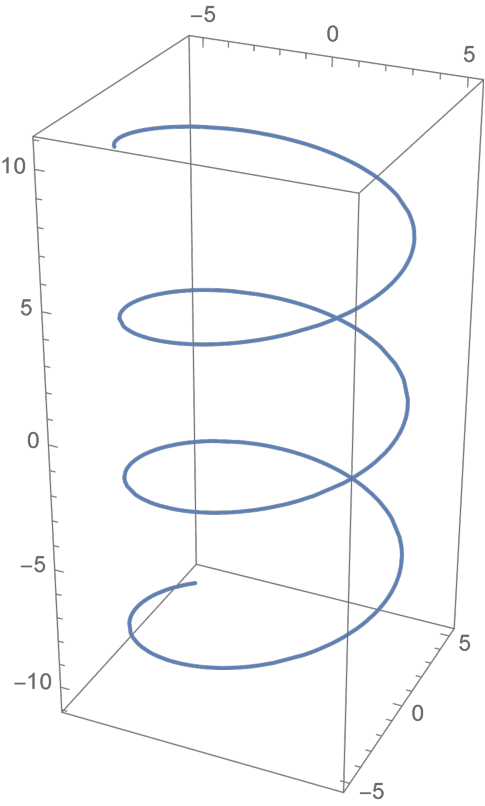
\includegraphics[width=0.3\textwidth]{images/simple_helix.pdf}
	% \caption[caption za v kazalo]{Dolg caption pod sliko}
	  \caption[Primer preposte vijačnice]{Na sliki je razviden graf vijačnice $\rV(t)=(5\cos{t},\sin{t},t).$ Os vrtenja predstavlja vektor $\aV=(0,0,1).$ Zlahka lahko po formuli \eqref{pogoj_vijacnica} preverimo, da je kot med osjo $\aV$ in enotsko tangento $\tV$ enak $\pi/4$ za vsak $t.$}
	  \label{fig:simple_helix}
	\end{figure}

Zanimivo dejstvo o vijačnicah, ki nam bo prišlo prav kasneje, je Lancretov izrek \cite{kreyszig2019differential}.
\begin{izrek}[Lancret]
	\label{lancret}
	Krivulja z neničelno fleksijsko ukrivljenostjo je vijačnica natanko takrat, ko je za vse njene točke razmerje med torzijsko in fleksijsko ukrivljenostjo konstantno.
\end{izrek}
\begin{proof}
	Naj bo krivulja $\rV(s)$ vijačnica izražena v naravni parametrizaciji. Torej drži enačba \eqref{pogoj_vijacnica} za nek vektor $\aV$ in kot $\psi.$ Če to enačbo odvajamo po $s$ in upoštevamo \eqref{eq2_5}, dobimo
	\begin{equation*}
		\aV \cdot \tV'=\kappa \aV \cdot \pV=0.
	\end{equation*}
	Zaradi predpostavke in nenegativnosti $\kappa$ sledi, da je $\kappa > 0.$ Torej mora veljati
	\begin{equation}
	\label{eq4_19}
	\aV \cdot \pV=0.
	\end{equation}
	To pomeni, da je v vsaki točki na krivulji enotska normala pravokotna na os vrtenja $\aV.$ Vektor $\aV$ se torej ves čas nahaja v ravnini, ki jo razpenjati enotska tangenta $\tV$ ter enotska binormala $\bV.$ Če velja formula \eqref{pogoj_vijacnica}, je potem iz slike \ref{fig:lancret} razvidno, da mora veljati tudi
	\begin{equation*}
		\aV \cdot \bV=\sin \psi.
	\end{equation*}
	\begin{figure}[h!]
	  \centering
	  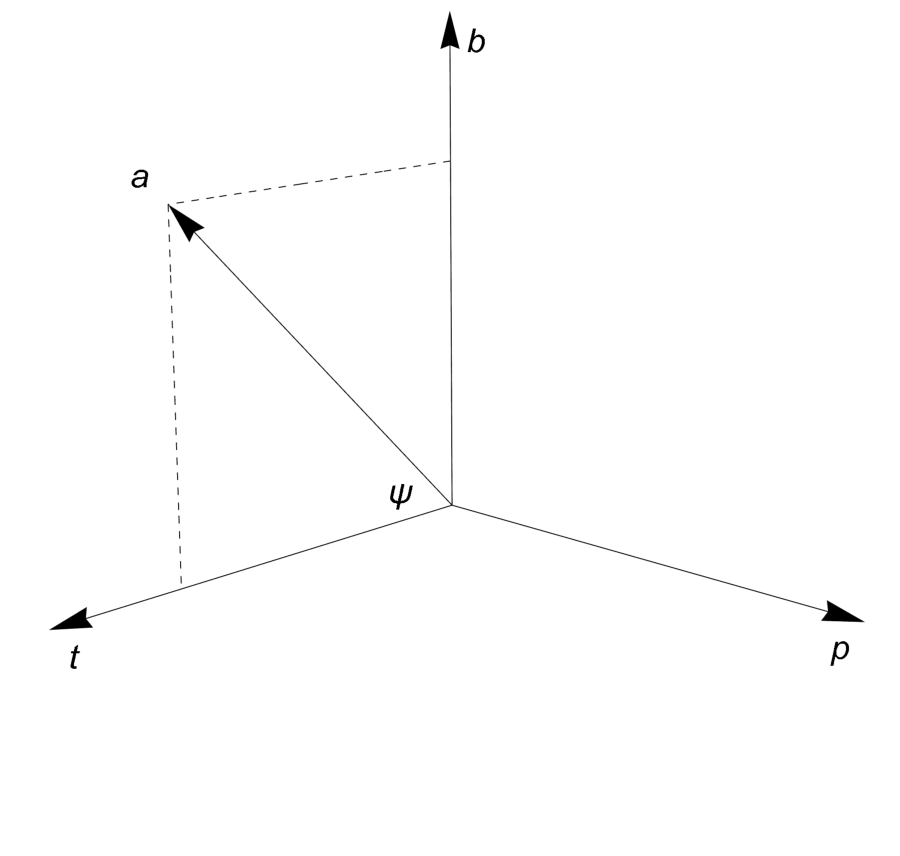
\includegraphics[width=0.5\textwidth]{images/lancret.pdf}
	% \caption[caption za v kazalo]{Dolg caption pod sliko}
	  \caption[Os vijačnice v primerjavi z enotsko tangento, normalo in binormalo]{Os vijačnice v primerjavi z enotsko tangento, normalo in binormalo.}
	  \label{fig:lancret}
	\end{figure}
	
	Sedaj odvajajmo enačbo \eqref{eq4_19} in upoštevamo Frenetovo formulo za odvod enotske normale v naravni parametrizaciji \eqref{naravne_frenetove_formule}. Dobimo naslednji izraz:
	\begin{equation*}
		\aV \cdot \pV'=\aV \cdot (-\kappa \tV+\tau \bV)=-\kappa \cos \psi + \tau \sin \psi=0.
	\end{equation*}
	Torej je $\frac{\tau(s)}{\kappa(s)}=\cot \psi,$ kar je res konstantna vrednost.
	
	Dokažimo izrek še v drugo smer. Predpostavimo, da je za krivuljo $\rV,$ podano v naravni parametrizaciji, razmerje med torzijsko in fleksijsko krivuljo konstanto
	$$\frac{\tau(s)}{\kappa(s)}=c_0,$$
	kjer je $c_0\in\R.$ Velja torej $c_0\kappa-\tau=0.$ Ob upoštevanju \eqref{naravne_frenetove_formule}, vidimo, da velja
	$$c_0\tV'+\bV'=(c_0\kappa-\tau)\pV=0.$$
	Ko ta izraz integriramo, dobimo $c_0\tV+\bV=\cV^*,$ kjer je $\cV^*$ neničelen konstanten vektor. Če ta vektor normaliziramo, dobimo
	$$\cV=\frac{\cV^*}{\lVert\cV^*\rVert}=\frac{c_0\tV+\bV}{\sqrt{1+c_0^2}}.$$
	Sedaj lahko skalarno pomnožimo vektor $\cV$ z enotsko tangento $\tV.$ Dobimo
	$$\cV\cdot\tV=\frac{c_0}{\sqrt{1+c_0^2}}.$$
	Po Pitagorovem izreku je jasno, da je ta skalarni produkt strogo manjši od 1. Torej enotska tangenta $\tV$ oklepa konstanten kot s konstantnim vektorjem $\cV.$ Sledi, da je krivulja $\rV$ vijačnica, kar pa je tisto, kar smo želeli dokazati.
\end{proof}
Naslednja trditev nam bo osvetila povezavo med vijačnimi polinomskimi krivuljami (vijačnicami, ki so hkrati tudi polinomske krivulje) in PH krivuljami \cite{faroukietal2004}.
\begin{trditev}
	\label{trditev_vijacnica_PH}
	Če je polinomska krivulja vijačnica, ima potem tudi pitagorejski hodograf.
\end{trditev}
\begin{proof}
	Za prostorko krivuljo $\rV$ lahko njeno enotsko tangento zapišemo kot $\frac{\rV'}{\lVert \rV' \rVert}.$ Potem lahko enačbo \eqref{pogoj_vijacnica} preoblikujemo kot
	\begin{equation}
		\aV \cdot \rV'(t)=\cos \psi \lVert \rV'(t) \rVert.
	\end{equation}
	Leva stran enačba predstavlja polinom v spremenljivki $t.$ Na desni strani enačbe se lahko nahaja polinom le, če je $\rV$ PH krivulja, kajti po definiciji so PH krivulje tiste krivulje, ki imajo hitrost $\lVert \rV' \rVert$ v polinomski odvisnosti od parametra $t.$
\end{proof}
Če je krivulja polinomska vijačnica, potem je tudi PH krivulja. Ali velja tudi obratno? Odgovor na to vprašanje je negativen, kot lahko vidimo iz spodnjega primera \cite{beltranmonterde}.
\begin{primer}
	\label{PH_ne_vijacnica}
	\textbf{.} Dana je naslednja krivulja
	\begin{equation*}
		\rV(t)=\left ( \frac{t^7}{21}+\frac{t^5}{5}+t^3-3t,-\frac{t^4}{2}+3t^2,-2t^3 \right ).
	\end{equation*}
	Če izračunamo njeno parametrično hitrost in količino $\lVert \rV' \times \rV'' \rVert,$ dobimo
	\begin{equation*}
		\lVert \rV'(t) \rVert=\frac{1}{3}(t^6+3t^4+9t^2+9) \quad \text{in} \quad \lVert \rV' \times \rV'' \rVert=2(t^2+1)(t^6+3t^4+9t^2+9).
	\end{equation*}
	Vidimo, da je krivulja res PH krivulja. Če upoštevamo formuli \eqref{kappa1} ter \eqref{tau1} in izračunamo razmerje
	\begin{equation*}
		\frac{\tau(t)}{\kappa(t)}=\frac{2t^6+9t^4-9}{9(t^2+1)^2},
	\end{equation*}
	pa po Lancretovemu izreku \ref{lancret} sledi, da krivulja $\rV$ ne more biti vijačnica, saj razmerje med torzijsko in fleksijsko ukrivljenostjo ni konstantno.
\end{primer}

Lancretov izrek nam omogoča, da za polinomsko vijačnico še drugače izrazimo količino $\rho,$ ki nastopa v enačbi \eqref{eq4_13}. Razmerje med fleksijsko \eqref{kappa1} in torzijsko \eqref{tau1} ukrivljenostjo je enako
\begin{equation}
	\label{rho3over2}
	\frac{\kappa}{\tau}=\frac{\fleksija}{\torzija}=\frac{(\sigma \sqrt{\rho})^3}{\sigma^3(\rV'\times\rV'')\cdot\rV'''}=\frac{\rho^{3/2}}{(\rV'\times\rV'')\cdot\rV'''}=\tan \psi.
\end{equation}
Iz tega lahko sklepamo, da je PH krivulja polinomska vijačnica tedaj, ko je izpolnjen pogoj $\rho^{3/2}=\tan \psi (\rV'\times\rV'')\cdot\rV'''.$

\subsection{Izražanje prostorskih PH krivulj v kvaternionski obliki}
\label{PH_kvaternioni}

Za študij PH krivulj je zelo prikladna kvaternionska predstavitev le-teh. To obliko so najprej opisali avtorji v \cite{choi2002clifford}. Spomnimo se predstavitve regularne PH krivulje $\rV$ s pomočjo polinomov $u,v,p$ in $q.$ Če so ti polinomi stopnje največ $m,$ je potem PH krivulja, ki jo pridobimo z integriranjem hodografa $\rV',$ lihe stopnje, ki je enaka $n=2m+1.$

Tvorimo kvaternionski polinom na naslednji način
\begin{equation}
	\AQ(t)=u(t)+v(t)\iV+p(t)\jV+q(t)\kV.
\end{equation}
Če kvaternione z ničelnim skalarnim delom identificiramo z vektorji v $\R^3,$ kot smo opisali v poglavju \ref{kvaternioni_poglavje}, ugotovimo, da lahko enačbe \eqref{eq4_7} precej bolj kompaktno zapišemo s pomočjo zgornjega polinoma. Izračunamo
\begin{align}
	\AQ(t)\iV\AQ^*(t)=&[u^2(t)+v^2(t)-p^2(t)-q^2(t)]\iV, \nonumber \\
	&+2[u(t)q(t)+v(t)p(t)]\jV, \label{kvaternion} \\
	&+2[v(t)q(t)-u(t)p(t)]\kV, \nonumber
\end{align}
kjer je
\begin{equation}
	\AQ^*(t)=u(t)-v(t)\iV-p(t)\jV-q(t)\kV
\end{equation}
konjugirana vrednost polinoma $\AQ(t).$ Če primerjamo formuli \eqref{eq4_7} in \eqref{kvaternion}, opazimo, da velja $\rV'(t)=\AQ(t)\iV\AQ^*(t).$ Kvaternionski polinom $\AQ$ lahko izrazimo tudi v Bernsteinovi obliki
\begin{equation}
	\AQ(t)=u(t)+v(t)\iV+p(t)\jV+q(t)\kV=\sum_{\ell=0}^m\AQ_{\ell} \binom{m}{\ell}(1-t)^{m-\ell}t^{\ell},
\end{equation}
kjer so z $\AQ_{\ell}\in\quat$ označeni Bernsteinovi koeficienti, ki so enaki
\begin{equation}
	\label{bern_koef_quat}
	\AQ_{\ell}=u_{\ell}+v_{\ell}\iV+p_{\ell}\jV+q_{\ell}\kV \quad \text{za} \quad \ell=0,\dots m.
\end{equation}
Pri tem $u_{\ell},v_{\ell},p_{\ell},q_{\ell},$ $\ell=0,\dots m$ predstavljajo Bernsteinove koeficiente za vsakega od polinomov $u,v,p,q$ posebej. Parametrična hitrost krivulje $\rV$ se prav tako preprosto izrazi kot
\begin{equation}
	\label{kvaternionska_hitrost}
	\lVert \rV'(t) \rVert=\sigma(t)=\lVert \AQ(t) \rVert^2=\AQ(t) \AQ^*(t)=u^2(t)+v^2(t)+p^2(t)+q^2(t).
\end{equation}

Spomnimo se sedaj definicije \ref{primitiven_hodo} o primitivnem pitagorejskem hodografu. Če je največji skupni delitelj komponent hodografa nekonstanten, je torej enak nekemu polinomu $h,$ ki je sode stopnje brez realnih ničel. Potem se lahko tak ``neprimitiven'' hodograf zapiše kot
\begin{equation}
	\label{Bkvaternion}
	\rV'(t)=h(t)\BQ(t)\iV\BQ^*(t)
\end{equation}
za nek kvaternionski polinom $\BQ(t)$ stopnje $m-r,$ kjer je $h$ polinom stopnje $\st(h)=2r.$

\subsection{Izražanje prostorskih PH krivulj s Hopfovo preslikavo}
\label{hopf_poglavje}

Poleg kvaternionske oblike poznamo še drugi način za izražanje prostorskih PH krivulj, in sicer s Hopfovo preslikavo. Definiramo jo na naslednji način.
\begin{definicija}
	\label{hopf_def}
	\emph{Hopfova preslikava} $H$ je preslikava, ki slika iz $\C \times \C \to \R^3$ in je za $\balpha, \bbeta \in \C$ določena z naslednjim predpisom:
	\begin{equation}
		\label{hopf}
		\hopf(\balpha, \bbeta)=(|\balpha|^2-|\bbeta|^2,2\ReC(\balpha \bar{\bbeta}),2\ImC(\balpha \bar{\bbeta})).
	\end{equation}
\end{definicija}
S pomočjo že znanih polinomov $u(t),$ $v(t),$ $p(t)$ in $q(t)$ lahko definiramo kompleksna polinoma $\balpha(t)=u(t)+\iu v(t)$ ter $\bbeta(t)=q(t)+\iu p(t).$ Z malo računanja ugotovimo, da velja ravno $\rV'(t)=H(\balpha(t),\bbeta(t)).$

Parametrična hitrost ima v Hopfovi predstavitvi enostaven zapis, in sicer $$\lVert \rV'(t) \rVert=|\balpha(t)|^2+|\bbeta(t)|^2.$$ Kot bomo videli v nadaljevanju, je Hopfova oblika primernejša za obravnavo dvojnih PH krivulj.

\subsubsection{Pretvorba med predstavitvama}

Spoznali smo dva načina, kako izraziti hodograf PH krivulje: s pomočjo kvaternionske predstavitve ter predstavitve s Hopfovo preslikavo. Pretvorba med eno in drugo predstavitvijo je dokaj enostavna. Če identificiramo imaginarno enoto v kompleksnih številih $\iu$ z imaginarno enoto $\iV$ v kvaternionih, vidimo, da se do kvaternionske oblike $\AQ(t)=u(t)+v(t)\iV+p(t)\jV+q(t)\kV$ da priti s pomočjo kompleksnih polinomov $\balpha(t)=u(t)+\iu v(t)$ in $\bbeta(t)=q(t)+\iu p(t)$ na naslednji način:
\begin{align}
	\balpha(t)+\kV\bbeta(t) &= u(t)+\iu v(t)+\kV(q(t)+ \iu p(t)) \nonumber \\
	&=u(t)+v(t)\iV + p(t)\jV+ q(t)\kV \label{comp_to_quat} \\
	&= \AQ(t).\nonumber
\end{align}

Tudi kompleksna polinoma $\balpha(t)$ in $\bbeta(t)$ ni težko pridobiti iz kvaternionskega polinoma $\AQ(t).$ Hitro se da preveriti, da res velja
\begin{equation}
	\label{quat_to_comp}
		\balpha(t) = \frac{1}{2}\big(\AQ(t)-\iV\AQ(t)\iV\big) \quad \text{in} \quad \bbeta(t)= \frac{1}{2}\kV\big(\AQ(t)+\iV\AQ(t)\iV\big).
\end{equation}

\begin{opomba}
	Za dani hodograf $\rV'(t)=(x'(t),y'(t),z'(t))$ je možno pridobiti enoparametrsko družino kvaternionskih polinomov. Ker je $\rV'=\AQ\iV\AQ^*,$ je po lemi \ref{QiQ_enacba_lema} kvaternionski polinom $\AQ$ enak
	\begin{align*}
		\AQ(t)=\sqrt{\frac{1}{2}(\sigma(t)+x'(t))}\Big(&-\sin\phi+\cos\phi\iV+\frac{y'(t)\cos\phi+z'(t)\sin\phi}{\sigma(t)+x'(t)}\jV\\
		&+\frac{z'(t)\cos\phi-y'(t)\sin\phi}{\sigma(t)+x'(t)}\kV\Big),
	\end{align*}
	kjer je $\phi$ prost parameter. Prav tako lahko preko pretvorbe \eqref{quat_to_comp} vidimo, da je za dani hodograf možno pridobiti enoparametrsko družino kompleksnih polinomov $\balpha$ in $\bbeta,$ ki ustrezajo danemu hodografu:
	\begin{align*}
		\balpha(t)&=\sqrt{\frac{1}{2}(\sigma(t)+x'(t))}\big(-\sin\phi+\iu\cos\phi\big),\\
		\bbeta(t)&=\frac{\big(z'(t)\cos\phi-y'(t)\sin\phi\big)+\iu\big(y'(t)\cos\phi+z'(t)\sin\phi\big)}{\sqrt{2(\sigma(t)+x'(t))}}.
	\end{align*}
\end{opomba}

%%%%%%%%%%%%%%%%%%%%%%%%%%%%%%%%%%%%%%%%%%%%%%%%%%%%%%%%%%%%%%%%%%%%%
\section{Dvojne PH krivulje}

Kot smo že videli v poglavju \ref{subsec_lastnosti}, za krivuljo $\rV$ s pitagorejskim hodogram v splošnem tangenta $\tV$ in torzijska ukrivljenost $\tau$ sta racionalni funkciji parametra krivulje, normala $\pV,$ binormala $\bV$ ter fleksijska ukrivljenost $\kappa$ pa niso, saj vsebujejo člen $\lVert \rV' \times \rV'' \rVert,$ ki je v splošnem koren nekega polinoma. Zanimajo nas pogoji, pri katerih so vse omenjene količine racionalne funkcije parametra krivulje, torej Frenetovo ogrodje $(\tV,\pV,\bV)$ in obe ukrivljenosti $\kappa$ in $\tau.$

Iz enačbe \eqref{eq4_12} je moč razbrati naslednje: če je količina $\rho(t)$ popolni kvadrat, je potem tudi količina $\lVert \rV'(t) \times \rV''(t) \rVert$ polinom in ne koren nekega polinoma, kar potem vodi do racionalne odvisnosti Frenetovega ogrodja ter ukrivljenosti od parametra $t.$
\begin{definicija}
	\label{dvojnaPH}
	Za prostorsko polinomsko krivuljo $\rV$ pravimo, da je \emph{dvojna PH krivulja,} če sta tako $\lVert \rV' \rVert$ kot $\lVert \rV' \times \rV'' \rVert$ polinomski funkciji parametra $t,$ torej če sta izpolnjena pogoja
	\begin{equation}
		\lVert \rV' \rVert^2=x'^2+y'^2+z'^2=\sigma^2,
	\end{equation}
	\begin{equation}
		\label{DPH_pogoj}
		\lVert \rV' \times \rV'' \rVert^2=(y'z''-y''z')^2+(z'x''-z''x')^2+(x'y''-x''y')^2=(\sigma \omega)^2
	\end{equation}
	za neka polinoma $\sigma$ in $\omega.$
\end{definicija}
Na kratko jim bomo rekli kar \emph{DPH krivulje}, pogoju \eqref{DPH_pogoj} pa \emph{DPH pogoj}. Vsaka DPH krivulja je očitno tudi PH krivulja. Na DPH pogoj lahko pogledamo tudi s pomočjo karakterizacije PH krivulj s polinomi $u,v,q$ in $p.$ Količina $\rho$ v enačbi \eqref{rho2} mora biti enaka kvadratu nekega polinoma $\omega.$ Zapišimo sedaj formule za Frenetovo ogrodje in ukrivljenosti pri DPH krivuljah:
\begin{align}
	\tV&=\frac{\rV'}{\sigma}, \nonumber \\
	\pV&=\frac{\rV'\times \rV''}{\lVert \rV'\times \rV'' \rVert} \times \tV =\frac{\rV'\times \rV''}{\sigma \omega}\times \frac{\rV'}{\sigma}=\frac{(-\rV'' \cdot \rV')\rV'+\sigma^2\rV''}{\sigma^2\omega} \nonumber \\
	&=\frac{-((\sigma'\tV+\sigma \kappa \pV)\cdot(\sigma\tV))\rV'+\sigma^2\rV''}{\sigma^2\omega}=\frac{\sigma\rV''-\sigma'\rV'}{\sigma\omega},\label{DPH_frenet_ukrv} \\
	\bV&=\frac{\rV'\times \rV''}{\lVert \rV'\times \rV'' \rVert}=\frac{\rV'\times \rV''}{\sigma\omega}, \nonumber \\
	\kappa &= \frac{\lVert \rV'\times \rV'' \rVert}{\sigma^3}=\frac{\omega}{\sigma^2}, \nonumber \\
	\tau &= \frac{(\rV'\times\rV'')\cdot\rV'''}{\lVert \rV'\times \rV'' \rVert^2}=\frac{(\rV'\times\rV'')\cdot\rV'''}{\sigma^2\omega^2}.\nonumber
\end{align}
Če si še enkrat ogledamo enačbo \eqref{rho2}
\begin{equation}
	\label{rho_omega2}
	\rho=4[(up'-u'p+vq'-v'q)^2+(uq'-u'q-vp'+v'p)^2]=\omega^2,
\end{equation}
vidimo, da polinomi $2(up'-u'p+vq'-v'q),$ $2(uq'-u'q-vp'+v'p)$ in $\omega$ tvorijo pitagorejsko trojico. Po opombi \ref{opomba1} mora biti trojica naslednje oblike
\begin{align}
	up'-u'p+vq'-v'q&=h(a^2-b^2), \nonumber \\
	uq'-u'q-vp'+v'p&=2hab, \label{kubota} \\
	\omega&=2h(a^2+b^2), \nonumber
\end{align}
za polinome $h,a,b$ kjer sta si $a$ in $b$ tuja. Če sta si tudi polinoma $up'-u'p+vq'-v'q$ in $uq'-u'q-vp'+v'p$ tuja, lahko potem vzamemo $h\equiv 1.$ V takem primeru pravimo, da imamo \emph{primitivno} pitagorejsko trojico.

\subsection{DPH krivulje in vijačnice}
\label{sec_DPH_in_vijacnice}

V trditvi \ref{trditev_vijacnica_PH} smo pokazali, da so vse polinomske vijačnice hkrati tudi PH krivulje. Da se pokazati še več.
\begin{trditev}
	\label{trditev_vijacnica_DPH}
	Če je polinomska krivulja vijačnica, potem je tudi DPH krivulja.
\end{trditev}
\begin{proof}
	Dokaz je povzet po \cite{beltranmonterde}. Naj bo $\rV$ polinomska vijačnica, ki ima os v smeri enotskega vektorja $\aV.$ Po \eqref{pogoj_vijacnica} je $\aV\cdot\tV=\cos \psi=k,$ kjer smo s $k \in \R$ poudarili, da je ta skalarni produkt med $\aV$ in $\tV$ enak konstanti vrednosti. Iz dokaza izreka \ref{lancret} lahko sklepamo, da velja tudi $\aV\cdot\bV=\sqrt{1-k^2}.$ Ker velja $\tV=\frac{\rV'}{\lVert \rV' \rVert}$ in $\bV=\binormala,$ lahko oba skalarna produkta preoblikujemo ter dobimo
	\begin{equation}
		\aV\cdot\rV'=k\ndr \quad \text{in} \quad \aV\cdot (\rV'\times\rV'')=\sqrt{1-k^2}\ndrtddr .
	\end{equation}
	Po istem razmisleku kot pri dokazu trditve \ref{trditev_vijacnica_PH} vidimo, da sta levi strani obeh zgornjih enačb enaki polinomu, kar pomeni, da morata biti tudi desni strani polinomski. Tako je poleg hitrosti $\ndr$ tudi količina $\ndrtddr$ enaka polinomu, torej je izpolnjen DPH pogoj. Pokazali smo, da je krivulja $\rV$ res DPH krivulja.
\end{proof}

Za DPH krivuljo tretje in pete stopnje velja tudi obrat trditve: vsaka polinomska DPH krivulja tretje ali pete stopnje je vijačnica. Dokaz vsebuje kar nekaj podrobnosti in je dostopen v \cite{beltranmonterde}. Iz primera \ref{PH_ne_vijacnica} tudi vidimo, da je krivulja $\rV$ pravzaprav DPH krivulja. Ker je razmerje med ukrivljenostima nekonstanto, potem ta DPH krivulja sedme stopnje ni vijačnica, torej omenjena obratna trditev v splošnem ne drži za krivulje višjih stopenj.

Iz enačbe \eqref{rho3over2} je razvidno, da je za DPH krivulje razmerje med fleksijsko in torzijsko ukrivljenostjo enako
\begin{equation}
	\label{DPH_razmerje_ukrv_omega_mesani}
	\frac{\kappa}{\tau}=\frac{\omega^3}{(\rV'\times\rV'')\cdot\rV'''}=\tan\psi.
\end{equation}
Če je polinomska krivulja $\rV$ vijačnica, je po trditvi \ref{trditev_vijacnica_DPH} hkrati tudi DPH krivulja in zato mora biti po Lancretovem izreku \ref{lancret} razmerje med $\omega^3$ in $(\rV'\times\rV'')\cdot\rV'''$ konstantno. Če je stopnja PH krivulje enaka $n,$ je potem stopnja polinoma $\rho	$ enaka $2n-6,$ kot smo videli v trditvi \ref{stopnja_rho_trditev}. Iz tega sledi, da je $\st(\omega)=n-3.$

To pomeni, da je razmerje med ukrivljenostima za kubične PH krivulje vedno konstantno, saj sta tako obe količini $\omega^3$ in $(\rV'\times\rV'')\cdot\rV'''$ konstantni. Slednje lahko preverimo po daljšem, a elementarnem računanju. Torej lahko sklepamo, da je vsaka kubična PH krivulja hkrati vijačnica in tako tudi DPH krivulja.
\begin{primer}
	\textbf{.} Dana je krivulja $\rV(t)=(\frac{1}{3}t^3-t,\frac{2}{3}t^3-2t^2+2t,-\frac{2}{3}t^3+t^2-2t).$ Hitro lahko vidimo, da je njen hodograf enak $\rV'(t)=(t^2-1,2t^2-4t+2,-2t^2+2t-2).$ Z nekaj računanja ni težko preveriti, da je parametrična hitrost te krivulje enaka
	$$\sigma(t)=3t^2-4t+3,$$
	torej imamo res opravka s PH krivuljo. Izračunajmo še $\rV'\times\rV'':$
	$$\rV'(t)\times\rV''(t)=\big(4(t^2-1),2(t^2-4t+1),4(t-1)^2\big).$$
	Preverimo lahko, da je kvadrat norme zgornjega vektorskega produkta enak
	$$\lVert\rV'(t)\times\rV''(t)\rVert^2=4(3t^2-4t+3)^2=4\sigma^2(t).$$
	Po \eqref{DPH_pogoj} je potem naša krivulja DPH krivulja in velja $\omega\equiv2,$ torej je tudi $\omega^3$ konstantna funkcija. Izračunajmo sedaj še mešani produkt $(\rV'\times\rV'')\cdot\rV'''.$ Enak je
	$$\big(\rV'(t)\times\rV''(t)\big)\cdot\rV'''(t)=-16.$$
	Po enačbi \eqref{DPH_razmerje_ukrv_omega_mesani} je potem razmerje med fleksijsko in torzijsko ukrivljenostjo enako $-\frac{1}{2}.$ Tako smo za to PH krivuljo stopnje 3 videli, da je hkrati tudi vijačnica in DPH krivulja.
\end{primer}

Za PH krivulje stopnje 5 prav tako velja, da so DPH krivulje \cite[Izrek 1]{beltranmonterde}, torej za njih velja 
\begin{equation}
	\label{mesani_kotangens_omega}
	(\rV'\times\rV'')\cdot\rV'''=\cot\psi\ \omega^3.
\end{equation}
\begin{primer}
	\textbf{.} Dana je krivulja $\rV(t)=(-t^4+\frac{2}{3}t^3-t,\frac{8}{5}t^5-3t^4+4t^3-3t^2+2t,t^4-\frac{8}{3}t^3+3t^2-2t).$ Njen hodograf je potem enak $$\rV'(t)=(-4t^3+2t^2-1,8t^4-12t^3+12t^2-6 t+2,4t^3-8t^2+6 t-2).$$ Izkaže se, da je parametrična hitrost te krivulje enaka
	$$\sigma(t)=8t^4-12t^3+14t^2-8t+3.$$
	Dana krivulja je PH krivulja. Podobno kot v prejšnjem primeru izračunamo $\rV'\times\rV'':$
	$$\rV'(t)\times\rV''(t)=\big(-8(t^2-2t)(2t^2-2t+1)^2,6(2t^2-2t+1)^2,-2(2t^2-2t+1)^2(4t^2+4t-3)\big).$$
	Potem je kvadrat norme zgornjega vektorskega produkta enak
	$$\lVert\rV'(t)\times\rV''(t)\rVert^2=8(2t^2-2t+1)^4(4t^2-2t+3)^2=\omega^2(t)\sigma^2().$$
	Po \eqref{DPH_pogoj} je potem naša krivulja DPH krivulja, ker lahko določimo $$\omega(t)=\sqrt{8}(2t^2-2t+1).$$ Tudi formula za stopnjo $\st(\omega)=n-3=5-3=2$ je izpolnjena. Sedaj si oglejmo še mešani produkt $(\rV'\times\rV'')\cdot\rV'''.$ Enak je
	$$\big(\rV'(t)\times\rV''(t)\big)\cdot\rV'''(t)=48(2t^2-2t+1)^3.$$
	Po enačbi \eqref{DPH_razmerje_ukrv_omega_mesani} je potem razmerje med fleksijsko in torzijsko ukrivljenostjo enako $\frac{\sqrt{2}}{3}.$ Tako smo za tudi to PH krivuljo stopnje 5 videli, da je hkrati tudi vijačnica in DPH krivulja.
\end{primer}

Če DPH krivulja sedme oziroma višje stopnje enakosti \eqref{mesani_kotangens_omega} za nek kot $\psi,$ je potem tudi vijačnica. To enakost se lahko uporablja kot ``sito'', ki ločuje vijačne od nevijačnih DPH krivulj stopenj 7 ali več.

\subsection{Kvaternionska predstavitev dvojnih PH krivulj}

Kot smo že videli v poglavju \ref{PH_kvaternioni} o izražanju PH krivulj v kvaternionski obliki, se lahko hodograf običajne PH krivulje $\rV$ izraža s pomočjo kvaternionskega polinoma $\AQ(t)$ kot $\rV'(t)=\AQ(t)\iV\AQ^*(t),$ parametrična hitrost pa kot $\sigma(t)=\lVert \AQ(t) \rVert^2.$ 

Sedaj bomo izpeljali izraz za $\rho,$ kot smo ga navedli v \eqref{rho2}. Začnemo z $$\rV''=\AQ'\iV\AQ^*+\AQ\iV\AQ'^*(t).$$ Če gledamo na $\rV'$ in $\rV''$ kot kvaterniona z ničelnim skalarnim delom, se potem njun vektorski produkt $\rV'\times\rV''$ izrazi kot polovica njunega produkta brez polovice njunega konjugiranega produkta, kot smo videli v \eqref{kvat_vekt_prod}. Tako imamo
\begin{equation*}
	\rV'\times\rV''=\frac{1}{2}\left ( (\AQ\iV\AQ^*)(\AQ'\iV\AQ^*+\AQ\iV\AQ'^*)-(\AQ'\iV\AQ^*+\AQ\iV\AQ'^*)^*(\AQ\iV\AQ^*)^* \right )
\end{equation*}
in ko ta izraz razpišemo in malce poenostavimo, dobimo
\begin{equation*}
	\rV'\times\rV''=\frac{1}{2}\left ( \AQ\iV(\AQ^*\AQ'-\AQ'^*\AQ)\iV\AQ'^*+\sigma(\AQ'\AQ^*-\AQ\AQ'^*) \right ).
\end{equation*}
Ker je $\sigma=\AQ\AQ^*=\AQ^*\AQ,$ je potem
\begin{equation*}
	\sigma'=\AQ'\AQ^*+\AQ\AQ'^*=\AQ'^*\AQ+\AQ^*\AQ'.
\end{equation*}
Člena $\AQ^*\AQ'-\AQ'^*\AQ$ in $\AQ'\AQ^*-\AQ\AQ'^*$ se lahko izrazita s pomočjo $\sigma',$ in sicer tako, da je $\AQ^*\AQ'-\AQ'^*\AQ=\sigma'-2\AQ'^*\AQ$ ter $\AQ'\AQ^*-\AQ\AQ'^*=\sigma'-2\AQ\AQ'^*.$ Če vstavimo ta dva izraza v izraz za $\rV'\times\rV''$ in upoštevamo $\sigma=\AQ\AQ^*,$ se nekaj členov pokrajša in ostane
\begin{equation*}
	\rV'\times\rV''=\AQ\iV\AQ^*\AQ'\iV\AQ^* + \sigma\AQ'\AQ^*=\AQ(\iV\AQ^*\AQ'\iV + \AQ^*\AQ')\AQ^*.
\end{equation*}
Če izrazimo $\AQ$ s polinomi $u,v,p$ in $q$ sta potem produkta $\AQ^*\AQ'$ in $\iV\AQ^*\AQ'\iV$ enaka
\begin{align*}
	\AQ^*\AQ'=&(uu'+vv'+pp'+qq')+(uv'-u'v-pq'+p'q)\iV \\
	&+(up'-u'p+vq'-v'q)\jV+(uq'-u'q-vp'+v'p)\kV, \\
	\iV\AQ^*\AQ'\iV=&-(uu'+vv'+pp'+qq')-(uv'-u'v-pq'+p'q)\iV \\
	&+(up'-u'p+vq'-v'q)\jV+(uq'-u'q-vp'+v'p)\kV.
\end{align*}
Vidimo, da se skalarni del v $\rV'\times\rV''$ (pričakovano) pokrajša. Pokrajša se tudi člen pri enoti $\iV,$ koeficienta pri enotah $\jV$ in $\kV$ pa sta enaka. Definiramo ju kot nova polinoma
\begin{align}
	f(t)=u(t)p'(t)-u'(t)p(t)+v(t)q'(t)-v'(t)q(t), \nonumber \\
	g(t)=u(t)q'(t)-u'(t)q(t)-v(t)p'(t)+v'(t)q(t). \label{polinoma_f_g}
\end{align}
 S pomočjo polinomov $f$ in $g$ zapišemo
\begin{equation}
	\label{drtddr}
	\rV'\times\rV''=2\AQ(f\jV+g\kV)\AQ^*.
\end{equation}
Spet izrazimo $\AQ$ z znanimi polinomi in nato produkt pomnožimo. Po daljšem izračunu in poenostavljanju izrazov dobimo
\begin{align*}
	\label{drtddr}
	\rV'\times\rV''=&2 \big (2((vp-uq)f+(up+vq)g)\iV+(2(u^2-v^2+p^2-q^2)f+2(pq-uv)g)\jV \\
	&+(2(uv+pq)f+(u^2-v^2-p^2+q^2)g)\kV \big ).
\end{align*}
Če si sedaj pogledamo še kvadrat norme vektorskega produkta $\rV'\times\rV''$, imamo najprej precej dolg izraz
\begin{align*}
	\lVert\rV'\times&\rV''\rVert^2=4 \Big( 4(vp-uq)^2f^2+8(vp-uq)(up+vq)fg+4(up+vq)^2g^2\\
	&+(u^2-v^2+p^2-q^2)^2f^2+4(u^2-v^2+p^2-q^2)(pq-uv)fg+4(pq-uv)^2g^2\\
	&+4(uv+pq)^2f^2+4(uv+pq)(u^2-v^2-p^2+q^2)fg+(u^2-v^2-p^2+q^2)^2g^2 \Big).
\end{align*}
Vidimo, da se mešani členi $fg$ uničijo, člena pri $f^2$ in $g^2$ pa se skupaj seštejeta ravno v $\sigma^2=(u^2+v^2+p^2+q^2)^2.$ Dobimo
\begin{equation}
	\lVert\rV'(t)\times\rV''(t)\rVert^2=4\sigma^2(t)\big(f^2(t)+g^2(t)\big).
\end{equation}
Tako smo končno pokazali, da res drži enačba \eqref{rho2}, saj sta kvadrata polinomov $f$ in $g$ natanko tista izraza, ki se pojavita v formuli za $\rho,$ podani z \eqref{rho2}. Opravka imamo s pravzaprav isto pitagorejsko trojico kot v \eqref{kubota}. Sklepamo, da morata biti polinoma $f$ in $g$ enaka
\begin{equation}
	\label{polinoma_f_in_g}
	f=h(a^2-b^2),\quad g=2hab,
\end{equation}
za neke polinome $a,b$ ter $h$, kjer sta si $a$ in $b$ tuja.

Vektorski produkt $\rV'\times\rV''$ lahko pri DPH krivuljah s pomočjo kvaternionskih polinomov zapišemo še malce bolj kompaktno. To si oglejmo v naslednji trditvi.
\begin{trditev}
	\label{drtddr_za_DPH}
	Naj bo $\rV$ DPH krivulja, določena s kvaternionskim polinomom $\AQ=u+v\iV+p\jV+q\kV.$ Potem se vektorski produkt $\rV'\times\rV''$ da izraziti s pomočjo kvaternionskega polinoma $\BQ$ kot $\rV'\times\rV''=h\BQ\iV\BQ^*$. Polinom $\BQ$ se izraža kot $\BQ=\AQ\CQ,$ kjer je $\CQ=-b+a\iV+a\jV+b\kV,$ polinomi $a,b$ in $h$ pa so znani iz \eqref{kubota}.
\end{trditev}
\begin{proof}
	Če upoštevamo enačbo \eqref{drtddr} za $\rV'\times\rV''$ ter enakost \eqref{polinoma_f_in_g} za $f$ in $g$, je potem vektorski produkt $\rV'\times\rV''$ enak
	\begin{equation}
		\rV'\times\rV''=h\big(2\AQ((a^2-b^2)\jV+2ab\kV)\AQ^*\big).
	\end{equation}
	Predpostavimo, da je $\rV'\times\rV''=h\BQ\iV\BQ^*$ in poskusimo določiti $\BQ.$ Če izraz $\BQ\iV\BQ^*$ pomnožimo z leve z $\AQ^*$ ter z desne z $\AQ,$ dobimo
	\begin{equation}
		\label{kvat_enacba_QiQ2}
		\QQ\iV\QQ^*=2\sigma^2\big((a^2-b^2)\jV+2ab\kV\big),
	\end{equation}
	kjer je $\QQ=\AQ^*\BQ.$ Po lemi \ref{QiQ_enacba_lema} ima splošna rešitev enačbe \eqref{kvat_enacba_QiQ2} obliko
	\begin{equation*}
		\QQ=\sigma\frac{((a^2+b^2)\iV+(a^2-b^2)\jV+2ab\kV)}{\sqrt{a^2+b^2}}(\cos\phi+\sin\phi\iV),
	\end{equation*}
	kjer je $\phi$ parameter, odvisen od parametra $t.$ Sledi, da je $\BQ$ enak
	\begin{equation*}
		\BQ=\AQ\frac{((a^2+b^2)\iV+(a^2-b^2)\jV+2ab\kV)}{\sqrt{a^2+b^2}}(\cos\phi+\sin\phi\iV).
	\end{equation*}
	Želimo, da je $\BQ(t)$ kvaternionski polinom, zato moramo izbrati  $\phi$ v odvisnosti od $t,$ pri kateremu to res drži. Implicitno definiramo $\phi(t)$ z naslednjima formulama
	\begin{equation*}
		\sin\phi(t)=\frac{b(t)}{\sqrt{a^2(t)+b^2(t)}}\quad\text{in}\quad\cos\phi(t)=\frac{a(t)}{\sqrt{a^2(t)+b^2(t)}}.
	\end{equation*}
	Vstavimo ta dva izraza v izraz za $\BQ(t)$ in poenostavimo
	\begin{align*}
		\BQ&=\AQ\left(-b+a\iV+\frac{a(a^2-b^2)+2ab^2}{a^2+b^2}\jV+\frac{2a^2b-b(a^2-b^2)}{a^2+b^2}\kV\right)\\
		&=\AQ(-b+a\iV+a\jV+b\kV)=\AQ\CQ.
	\end{align*}
	Torej res drži $\BQ=\AQ\CQ,$ kar smo hoteli dokazati.
\end{proof}

\subsection{Predstavitev dvojnih PH krivulj s Hopfovo preslikavo}

Za nadaljnjo obravnavo in klasifikacijo dvojnih PH krivulj se predstavitev le-teh s Hopfovo preslikavo izkaže za bolj primerno od predstavitve s kvaternionskim polinomom. Za kompleksna polinoma $\balpha(t)=u(t)+\iu v(t)$ in $\bbeta(t)=q(t)+\iu p(t)$ lahko podamo hodograf PH krivulje s pomočjo preslikave, kot smo že videli v poglavju \ref{hopf_poglavje}. Oglejmo si, čemu je enak polinom $\balpha(t)\bbeta'(t)-\balpha'(t)\bbeta(t):$
\begin{align}
	\balpha\bbeta'-\balpha'\bbeta&=(u+\iu v)(q'+\iu p')-(u'+\iu v')(q+\iu p) \nonumber \\
	&=(uq'-u'q+v'p-vp')+\iu(vq'-v'q+up'-u'p).
\end{align}
Če primerjamo kvadrat absolutne vrednosti te izračunane količine z enačbo \eqref{rho2}, vidimo da je
\begin{equation}
	\label{rho_propoly}
	\rho(t)=4|\balpha(t)\bbeta'(t)-\balpha'(t)\bbeta(t)|^2.
\end{equation}
Tu se nam ponudi nova karakterizacija DPH krivulj: DPH krivulje so tiste prostorske krivulje, za katere je $|\balpha(t)\bbeta'(t)-\balpha'(t)\bbeta(t)|^2$ popolni kvadrat nekega realnega polinoma. Izkaže se, da je polinom $\balpha(t)\bbeta'(t)-\balpha'(t)\bbeta(t)$ pomemben za nadaljnji študij DPH krivulj, zato si zasluži tudi svojo definicijo.
\begin{definicija}
	Polinomu $\balpha(t)\bbeta'(t)-\balpha'(t)\bbeta(t)$, ki ga sestavimo iz polinomov $\balpha(t)=u(t)+\iu v(t)$ ter $\bbeta(t)=q(t)+\iu p(t)$ za neke realne polinome $u(t),$ $v(t),$ $p(t)$ ter $q(t),$ pravimo tudi \emph{polinom proporcionalnosti} polinomov $\balpha(t)$ in $\bbeta(t)$ (angl.:\ \emph{proportionality polynomial}).
\end{definicija}
Enostavno je videti, da je polinom proporcionalnosti identično enak nič natanko takrat, ko se polinoma $\balpha$ in $\bbeta$ razlikujeta za kompleksno konstanto. V eno smer se to pokaže direktno, za dokaz v drugo smer se pa reši preprosto diferencialno enačbo.
S polinomom proporcionalnosti se da lepo izraziti tudi fleksijsko ukrivljenost DPH krivulj, in sicer kot
\begin{equation}
	\label{kappa_propoly}
	\kappa=\frac{\omega}{\sigma^2}=\frac{\sqrt{\rho}}{\sigma^2}=2\frac{|\balpha\bbeta'-\balpha'\bbeta|}{|\balpha|^2+|\bbeta|^2}.
\end{equation}
Iz tega je razvidno sledeče. Če je za dano DPH krivuljo njen polinom proporcionalnosti identično enak 0, je potem tudi fleksijska ukrivljenost te krivulje enaka 0, kar pomeni, da imamo pravzaprav opravka z daljico (ravno črto). Če ima ta polinom kakšno realno ničlo, lahko pri tej vrednosti parametra $t$ normalni oziroma binormalni vektor nista določena, saj tako normalni kot binormalni vektor vsebujeta v imenovalcu $\omega,$ kot lahko vidimo v enačbah \eqref{DPH_frenet_ukrv}. Podobno velja tudi za torzijsko ukrivljenost.

Sedaj lahko preoblikujemo DPH pogoj v primernejšo obliko za nadaljnjo obravnavo. Spomnimo se enakosti \eqref{kubota}. Če to primerjamo s polinomom proporcionalnosti, vidimo, da je
\begin{align}
	\balpha\bbeta'-\balpha'\bbeta&=(up'-u'p+v'q-vq')\nonumber \\
	&+\iu(uq'-u'q+vp'-v'p) \label{propor_poly_izpeljava} \\
	&=h(a^2-b^2+\iu 2ab) \nonumber \\
	&=h\wV^2 \nonumber
\end{align}
kjer je $\wV=a+\iu b.$ Polinoma $a$ in $b$ morata biti tuja, tako da velja tudi
\begin{equation}
	\st(h)+2\st(\wV)=\st(\balpha\bbeta'-\balpha'\bbeta)=\st(\balpha)+\st(\bbeta)-2.
	\end{equation}
Da je $\st(\balpha\bbeta'-\balpha'\bbeta)=\st(\balpha)+\st(\bbeta)-2,$ vemo iz opombe \ref{opomba_proporpoly}. Če identificiramo $\C$ z $\R^2,$ potem kompleksna polinoma $\balpha$ in $\bbeta$ porodita ravninske krivulje. Ob upoštevanju enakosti \eqref{poly_ravninska_PH} iz opombe \ref{opomba1} ter izpeljave \eqref{propor_poly_izpeljava} je jasno, da velja naslednja trditev.
\begin{trditev}
	Naj bo $\rV$ prostorska PH krivulja, podana s Hopfovo preslikavo polinomov $\balpha$ ter $\bbeta.$ Potem je $\rV$ DPH krivulja natanko takrat, ko polinom proporcionalnosti polinomov $\balpha$ in $\bbeta$ določa hodograf ravninske PH krivulje.
\end{trditev}

Iz enačbe \eqref{rho_propoly} za $\rho$ in karakterizacije DPH pogoja s pomočjo polinoma proporcionalnosti \eqref{propor_poly_izpeljava} sledi, da je za DPH krivulje $\rho$ enak $\rho=4h^2|\wV|^4,$ kjer je $\wV=a+\iu b,$ $a,b$ in $h$ pa so realni polinomi. Ker je po enačbi \eqref{rho_omega2} kvadrat polinoma $\omega$ enak polinomu $\rho$ in če predpostavimo, da je polinom $h$ nenegativen, je potem res $\omega=2h|\wV|^2.$ Kot smo že videli v poglavju \ref{sec_DPH_in_vijacnice}, je za vijačne DPH krivulje razmerje med mešanim produktom $(\rV'\times\rV'')\cdot\rV'''$ in kubom polinoma $\omega$ konstantno, zato je tudi razmerje med $(\rV'\times\rV'')\cdot\rV'''$ in $\big(2h|\wV|^2\big)^3$ konstantno.

Polinom proporcionalnosti se da izraziti tudi v jeziku kvaternionov. Najprej identificiramo imaginarno enoto $\iu$ v $\C$ z imaginarno enoto $\iV$ v $\quat.$ Polinoma $\balpha$ in $\bbeta$ lahko zapišemo v Bernsteinovi bazi s koeficienti
\begin{equation*}
	\balpha_\ell=\gamma_\ell+\delta_\ell\iV\quad\text{in}\quad\bbeta_\ell=\zeta_\ell+\eta_\ell\iV\quad\text{za}\quad \ell=0,\dots,m.
\end{equation*}
Bernsteinovi koeficienti kvaternionskega polinoma $\AQ$ so potem po pretvorbi \eqref{comp_to_quat} enaki
\begin{equation*}
	\AQ_\ell=\balpha_\ell+\kV\bbeta_\ell=\gamma_\ell+\delta_\ell\iV+\eta_\ell\jV+\zeta_\ell\kV
\end{equation*}
za $\ell=0,\dots,m.$ Kvaternion $\AQ_k^*\AQ_\ell-\AQ_\ell^*\AQ_k$ ima ničelni skalarni del in ga zato lahko identificiramo z vektorjem. Ko razpišemo izraz $\frac{1}{2}(\AQ_k^*\AQ_\ell-\AQ_\ell^*\AQ_k)\times\iV$ vidimo, da je enak
\begin{align*}
	\frac{1}{2}(\AQ_k^*\AQ_\ell-\AQ_\ell^*\AQ_k)\times\iV&=(\gamma_k\zeta_\ell+\eta_k\delta_\ell-\zeta_k\gamma_\ell-\delta_k\eta_\ell)\jV\\
	&+(\zeta_k\delta_\ell+\eta_k\gamma_\ell-\gamma_k\eta_\ell-\delta_k\zeta_\ell)\kV.
\end{align*}
Isti izraz dobimo, če poračunamo $\jV(\balpha_k\bbeta_\ell-\balpha_\ell\bbeta_k).$ Iz teh enakosti lahko sklepamo, da se da polinom proporcionalnosti polinomov $\balpha(t)$ in $\bbeta(t)$ izraziti s kvaternionskim polinom $\AQ(t)$ kot
\begin{equation}
	\label{propor_kot_quat}
	\jV\big(\balpha(t)\bbeta'(t)-\balpha'(t)\bbeta(t)\big)=\frac{1}{2}\big(\AQ^*(t)\AQ'(t)-\AQ'^*(t)\AQ(t)\big)\times\iV.
\end{equation}

S pomočjo pravkar izpeljanega izraza lahko tudi DPH pogoj \eqref{propor_poly_izpeljava} izrazimo malce drugače. Uporabimo polinom $\CQ(t)=-b(t)+a(t)\iV+a(t)\jV+b(t)\kV$ iz trditve \ref{drtddr_za_DPH}. Potem velja
\begin{equation*}
	\frac{1}{2}\CQ(t)\iV\CQ^*(t)=\big(a^2(t)-b^2(t)\big)\jV+2a(t)b(t)\kV=\wV^2(t)\jV.
\end{equation*}
Pomnožimo sedaj desno stran enačbe \eqref{propor_kot_quat} z desne z $\jV.$ Dobimo
\begin{align*}
	\left(\frac{1}{2}\big(\AQ^*(t)\AQ'(t)-\AQ'^*(t)\AQ(t)\big)\times\iV\right)\jV&=\jV\big(\balpha(t)\bbeta'(t)-\balpha'(t)\bbeta(t)\big)\jV\\
	&=h(t)\jV\wV^2(t)\jV\\
	&=\frac{1}{2}h(t)\jV\CQ(t)\iV\CQ^*(t).
\end{align*}
Rezultat lahko še lepše izrazimo v obliki
\begin{equation}
	\label{dvojnaPH_quat_pogoj}
	\big(\AQ^*(t)\AQ'(t)-\AQ'^*(t)\AQ(t)\big)\times\iV=h(t)\DQ(t)\iV\DQ^*(t),
\end{equation}
kjer je $\DQ(t)=\jV\CQ(t)=-a(t)+b(t)\iV-b(t)\jV-a(t)\kV.$ Če povzamemo: prostorska PH krivulja, podana s kvaternionskim polinomom $\AQ,$ je dvojna PH krivulja natanko takrat, ko drži zgornja enačba za nek kvaternionski polinom $\DQ,$ ki mora biti predpisane oblike, pri čimer sta si polinoma $a$ ter $b$ tuja.

%%%%%%%%%%%%%%%%%%%%%%%%%%%%%%%%%%%%%%%%%%%%%%%%%%%%%%%%%%%%%%%%%%%%

\section{Klasifikacija DPH krivulj nizkih stopenj}

V tem poglavju si bomo ogledali različne tipe DPH krivulj, ki se pojavljajo pri nizkih stopnjah. Analizirali bomo tipe krivulj pri tretji, peti in sedmi stopnji. Glavno orodje pri tej analizi bo Hopfova oblika DPH krivulj s polinomom proporcionalnosti. Izpeljali bomo pogoje (odvisne od koeficientov polinoma proporcionalnosti), pri katerih je dana PH krivulja tudi DPH krivulja. Pri tem bomo privzeli, da sta polinoma $\balpha$ in $\bbeta$ podana v Bernsteinovi obliki
\begin{equation*}
	\balpha(t)=\sum_{\ell=0}^m\balpha_\ell\binom{m}{\ell}(1-t)^{m-\ell}t^\ell\quad\text{in}\quad\bbeta(t)=\sum_{\ell=0}^m\bbeta_\ell\binom{m}{\ell}(1-t)^{m-\ell}t^\ell,
\end{equation*}
kjer je $m$ enak $m=\frac{n-1}{2},$ pri čimer je $n$ stopnja krivulje.

\subsection{Dvojne PH krivulje tretje in pete stopnje}

Naj bo $\rV$ prostorska PH krivulja tretje stopnje, podana s kompleksnima polinomoma $\balpha$ in $\bbeta.$ Potem sta oba kompleksna polinoma pravzaprav linearna $$\balpha(t)=\balpha_0(1-t)+\balpha_1t\quad\text{in}\quad\bbeta(t)=\bbeta_0(1-t)+\bbeta_1t.$$ Po krajšem računu hitro vidimo, da je polinom proporcionalnosti enak
\begin{align*}
	\balpha(t)\bbeta'(t)-\balpha'(t)\bbeta(t)&=\balpha_0\bbeta_1(1-t)-\balpha_0\bbeta_0(1-t)+\balpha_1\bbeta_1t-\balpha_1\bbeta_0t\\
	&-\balpha_1\bbeta_0(1-t)-\balpha_1\bbeta_1t+\balpha_0\bbeta_0(1-t)-\balpha_0\bbeta_1t\\
	&=\balpha_0\bbeta_1-\balpha_1\bbeta_0.
\end{align*}
Polinom proporcionalnosti je torej konstanten in je po \eqref{propor_poly_izpeljava} enak $h(t)\wV^2(t).$ Iz zgornjega računa vidimo, da je $\st(h)=\st(\wV)=0.$ Brez škode za splošnost lahko privzamemo, da je $h(t)\equiv1$ ter $\wV(t)=\wV_0$ za neko konstanto $\wV_0\in\C.$ Potem lahko DPH pogoj izrazimo kot $\balpha_0\bbeta_1-\balpha_1\bbeta_0=\wV_0^2.$ Ta pogoj jasno velja za vse možne izbire $\balpha_0,\balpha_1,\bbeta_0$ in $\bbeta_1,$ saj lahko za $\wV_0$ vzamemo $\pm\sqrt{\balpha_0\bbeta_1-\balpha_1\bbeta_0},$ ki je v kompleksnih številih vedno definirano število. Zato je vsaka prostorska PH krivulja tretje stopnje tudi dvojna PH krivulja.

Naj bo sedaj $\rV$ prostorska PH krivulja pete stopnje, ki je podana s kompleksnima polinomoma $\balpha$ in $\bbeta.$ V tem primeru sta ta dva polinoma kvadratična. Tokrat je polinom proporcionalnosti enak
\begin{align}
	\balpha(t)\bbeta'(t)-\balpha'(t)\bbeta(t)&=2(\balpha_0\bbeta_1-\balpha_1\bbeta_0)(1-t)^2+(\balpha_0\bbeta_2-\balpha_2\bbeta_0)2(1-t)t\nonumber\\
	&+2(\balpha_1\bbeta_2-\balpha_2\bbeta_1)t^2.\label{propoly_bern_5}
\end{align}
Krivulja je DPH krivulja, ko je zgornji izraz enak $h(t)\wV^2(t)$ za nek realen polinom $h(t)$ in nek kompleksni polinom $\wV(t).$ Tu ločimo dva primera: ali je $\st(h)=0$ in $\st(\wV)=1$ ali pa $\st(h)=2$ in $\st(\wV)=0.$

\subsubsection{Primer \texorpdfstring{$\st(h)=0$}{st(h)=0} in \texorpdfstring{$\st(\wV)=1$}{st(w)=1}}

Recimo, da je $\st(h)=0$ in $\st(\wV)=1.$ Kot prej lahko brez škode za splošnost privzamemo, da je $h(t)\equiv1,$ polinom $\wV(t)$ pa je enak $\wV(t)=\wV_0(1-t)+\wV_1t,$ torej je $\wV^2(t)=\wV_0^2(1-t)^2+\wV_0\wV_12(1-t)t+\wV_1^2t^2.$ Če enačimo koeficiente izraza $h(t)\wV^2(t)$ s koeficienti izraza \eqref{propoly_bern_5}, dobimo naslednje enačbe:
\begin{equation}
	2(\balpha_0\bbeta_1-\balpha_1\bbeta_0)=\wV_0^2,\quad \balpha_0\bbeta_2-\balpha_2\bbeta_0=\wV_0\wV_1,\quad 2(\balpha_1\bbeta_2-\balpha_2\bbeta_1)=\wV_1^2.
\end{equation}
Če pomnožimo prvo in tretjo enačbo, vidimo, da je zmnožek desnih strani enak kvadratu desne strani druge enačbe. Torej te enačbe res držijo za neka $\wV_0$ in $\wV_1$ natanko takrat, ko za koeficiente polinomov $\balpha$ in $\bbeta$ drži enačba
\begin{equation}
	\label{st5h0w1}
	4(\balpha_0\bbeta_1-\balpha_1\bbeta_0)(\balpha_1\bbeta_2-\balpha_2\bbeta_1)=(\balpha_0\bbeta_2-\balpha_2\bbeta_0)^2.
\end{equation}

\subsubsection{Primer \texorpdfstring{$\st(h)=2$}{st(h)=2} in \texorpdfstring{$\st(\wV)=0$}{st(w)=0}}

Oglejmo si še drugi primer, ko je $\st(h)=2$ in $\st(\wV)=0.$ Polinom $h(t)=h_0(1-t)^2+h_12(1-t)t+h_2t^2$ prav tako podamo v Bernsteinovi obliki, za $\wV(t)$ pa postavimo $\wV(t)\equiv\wV_0.$ Spet enačimo koeficiente izraza $h(t)\wV^2(t)$ s koeficienti izraza \eqref{propoly_bern_5}. Dobimo naslednji sistem enačb:
\begin{equation}
	2(\balpha_0\bbeta_1-\balpha_1\bbeta_0)=h_0\wV_0^2,\quad \balpha_0\bbeta_2-\balpha_2\bbeta_0=h_1\wV_0^2,\quad 2(\balpha_1\bbeta_2-\balpha_2\bbeta_1)=h_2\wV_0^2.\label{st5h2w0}
\end{equation}
Ta sistem enačb je rešljiv natanko takrat, ko kompleksna števila $\balpha_0\bbeta_1-\balpha_1\bbeta_0,$ $\balpha_0\bbeta_2-\balpha_2\bbeta_0$ ter $\balpha_1\bbeta_2-\balpha_2\bbeta_1$ ležijo na isti premici v kompleksni ravnini.

\subsection{Dvojne PH krivulje sedme stopnje}
\label{poglavje_dvojnePHkrivulje7}

Imejmo prostorsko PH krivuljo $\rV$ sedme stopnje, ki je podana s kompleksnima polinomoma $\balpha$ in $\bbeta.$ Tokrat sta ta dva polinoma kubična. Po daljšem a elementarnem računanju vidimo, da je polinom proporcionalnosti enak
\begin{align}
	\balpha(t)\bbeta'(t)-\balpha'(t)\bbeta(t)&=3(\balpha_0\bbeta_1-\balpha_1\bbeta_0)(1-t)^4+\frac{3}{2}(\balpha_0\bbeta_2-\balpha_2\bbeta_0)4(1-t)^3t\nonumber\\
	&+\frac{1}{2}(\balpha_0\bbeta_3-\balpha_3\bbeta_0)\frac{3}{2}(\balpha_1\bbeta_2-\balpha_2\bbeta_1)6(1-t)^2t^2\label{propoly_bern_7}\\
	&+\frac{3}{2}(\balpha_1\bbeta_3-\balpha_3\bbeta_1)4(1-t)t^3+3(\balpha_2\bbeta_3-\balpha_3\bbeta_2)t^4.\nonumber
\end{align}
Za izpolnitev DPH pogoja imamo tokrat tri možnosti: ali je $\st(h)=0$ in $\st(\wV)=2$ ali je $\st(h)=2$ in $\st(\wV)=1$ ali je $\st(h)=4$ in $\st(\wV)=0.$ Opozoriti velja na dejstvo, da vrednosti $\balpha_i\bbeta_j-\balpha_j\bbeta_i$ za $0\leq i,j\leq 3,$ kjer sta $i\neq j,$ ki se pojavljajo kot členi znotraj koeficientov polinoma proporcionalnosti, niso med seboj neodvisne. Za njih velja pogoj, ki mu bomo rekli \emph{pogoj kompatibilnosti}. Po tem pogoju za te vrednosti velja enakost
\begin{align}
	(\balpha_0\bbeta_1-\balpha_1\bbeta_0)(\balpha_2\bbeta_3-\balpha_3\bbeta_2)&=(\balpha_0\bbeta_2-\balpha_2\bbeta_0)(\balpha_1\bbeta_3-\balpha_3\bbeta_1)\nonumber\\
	&-(\balpha_1\bbeta_2-\balpha_2\bbeta_1)(\balpha_0\bbeta_3-\balpha_3\bbeta_0).\label{pogoj_kompatibilnosti}
\end{align}
Če levo in desno stran enakosti razpišemo, vidimo, da je enakost vselej izpolnjena za poljubne $\balpha_i,\bbeta_i,$ kjer je $i=0,1,2,3.$

\subsubsection{Primer \texorpdfstring{$\st(h)=0$}{st(h)=0} in \texorpdfstring{$\st(\wV)=2$}{st(w)=2}}
\label{klasifikacija_h0w2}

Lahko vzamemo kar $h(t)\equiv1.$ Naj ima kvadratičen kompleksni polinom $\wV$ Bernsteinove koeficiente $\wV_0,\wV_1$ in $\wV_2.$ Če ta polinom kvadriramo in primerjamo koeficiente s koeficienti v enačbi \eqref{propoly_bern_7}, dobimo naslednje enačbe:
\begin{align}
	3(\balpha_0\bbeta_1-\balpha_1\bbeta_0)&=\wV_0^2,\nonumber\\
	3(\balpha_0\bbeta_2-\balpha_2\bbeta_0)&=2\wV_0\wV_1,\nonumber\\
	(\balpha_0\bbeta_3-\balpha_3\bbeta_0)+3(\balpha_1\bbeta_2-\balpha_2\bbeta_1)&=\frac{2}{3}(2\wV_1^2+\wV_0\wV_2),\label{sistem_st7h0w2}\\
	3(\balpha_1\bbeta_3-\balpha_3\bbeta_1)&=2\wV_1\wV_2,\nonumber\\
	3(\balpha_2\bbeta_3-\balpha_3\bbeta_2)&=\wV_2^2.\nonumber
\end{align}
Vrednost $\balpha_1\bbeta_2-\balpha_2\bbeta_1$ označimo z $\zV.$ Potem se v zgornjih enačbah tretja enačba preoblikuje v $\balpha_0\bbeta_3-\balpha_3\bbeta_0=\frac{4}{3}\wV_1^2+\frac{2}{3}\wV_0\wV_2-3\zV.$ Sedaj uporabimo pogoj kompatibilnosti \eqref{pogoj_kompatibilnosti} in izrazimo vse člene s koeficienti polinoma $\wV$ in številom $\zV.$ Dobimo
\begin{equation*}
	\left(\frac{1}{3}\wV_0^2\right)\left(\frac{1}{3}\wV_2^2\right)=\left(\frac{2}{3}\wV_0\wV_1\right)\left(\frac{2}{3}\wV_1\wV_2\right)-\zV\left(\frac{4}{3}\wV_1^2+\frac{2}{3}\wV_0\wV_2-3\zV\right).
\end{equation*}
Ko to enačbo poenostavimo, vidimo, da imamo opravka s kvadratno enačbo v $\zV.$ Le-ta je enaka
\begin{equation*}
	27\zV^2-(12\wV_1^2+6\wV_0\wV_2)\zV+(4\wV_1^2-\wV_0\wV_2)\wV_0\wV_2=0.
\end{equation*}
Ker ima kvadratna enačba dve rešitvi, lahko vrednost $\zV=\balpha_1\bbeta_2-\balpha_2\bbeta_1$ podamo s pomočjo koeficientov $\wV_0,$ $\wV_1$ in $\wV_2$ kot
\begin{equation}
	\label{st7h0w2}
	\zV=\balpha_1\bbeta_2-\balpha_2\bbeta_1=\frac{1}{3}\wV_0\wV_2\quad\text{ali}\quad\zV=\balpha_1\bbeta_2-\balpha_2\bbeta_1=\frac{1}{9}(4\wV_1^2-\wV_0\wV_2).
\end{equation}
Na začetku lahko torej poljubno izberemo koeficiente $\wV_0,\wV_1$ in $\wV_2$ (in s tem polinom $\wV$) ter še tri koeficiente polinomov $\balpha$ in $\bbeta$ (recimo $\balpha_0,\balpha_1$ in $\bbeta_0$). Nato rešimo linearni sistem enačb \eqref{sistem_st7h0w2}. Zaradi dveh možnih rešitev za $\balpha_1\bbeta_2-\balpha_2\bbeta_1,$ kot lahko vidimo v \eqref{st7h0w2}, dobimo dve različni množici rešitev sistema \eqref{sistem_st7h0w2}. Potem so vse vrednosti Bernsteinovih koeficientov polinomov $\balpha$ in $\bbeta$ tako določene, da je prostorska PH krivulja, ki je porojena iz teh dveh kompleksnih polinomov, res DPH krivulja. Ker imamo dve različni množici rešitev sistema \eqref{sistem_st7h0w2}, tako dobimo tudi dve različna hodografa, ki določata DPH krivuljo.

\subsubsection{Primer \texorpdfstring{$\st(h)=2$}{st(h)=2} in \texorpdfstring{$\st(\wV)=1$}{st(w)=1}}
\label{klasifikacija_h2w1}

Vzamemo $h_0,h_1,$ $h_2$ za Bernsteinove koeficiente polinoma $h$ ter $\wV_0$ in $\wV_1$ za Bernsteinove koeficiente polinoma $\wV.$ Če poračunamo $h(t)\wV^2(t)$ in primerjamo Bernsteinove tega polinoma s koeficienti polinoma proporcionalnosti \eqref{propoly_bern_7}, dobimo naslednji sistem enačb:
\begin{align}
	3(\balpha_0\bbeta_1-\balpha_1\bbeta_0)&=h_0\wV_0^2,\nonumber\\
	3(\balpha_0\bbeta_2-\balpha_2\bbeta_0)&=h_1\wV_0^2+h_0\wV_0\wV_1,\nonumber\\
	(\balpha_0\bbeta_3-\balpha_3\bbeta_0)+3(\balpha_1\bbeta_2-\balpha_2\bbeta_1)&=\frac{1}{3}(h_2\wV_0^2+4h_1\wV_0\wV_1+h_0\wV_1^2),\label{sistem_st7h2w1}\\
	3(\balpha_1\bbeta_3-\balpha_3\bbeta_1)&=h_2\wV_0\wV_1+h_1\wV_1^2,\nonumber\\
	3(\balpha_2\bbeta_3-\balpha_3\bbeta_2)&=h_2\wV_1^2.\nonumber
\end{align}
Uporabimo isti trik kot že v prejšnjem primeru. Nastavimo $\zV=\balpha_1\bbeta_2-\balpha_2\bbeta_1.$ Potem je vrednost $\balpha_0\bbeta_3-\balpha_3\bbeta_0$ po tretji enačbi zgoraj enaka $\frac{1}{3}(h_2\wV_0^2+4h_1\wV_0\wV_1+h_0\wV_1^2)-3\zV.$ Spet uporabimo pogoj kompatibilnosti \eqref{pogoj_kompatibilnosti}. Dobimo enačbo
\begin{align*}
	\left(\frac{1}{3}h_0\wV_0^2\right)\left(\frac{1}{3}h_2\wV_1^2\right)&=\frac{1}{3}(h_1\wV_0^2+h_0\wV_0\wV_1)\frac{1}{3}(h_2\wV_0\wV_1+h_1\wV_1^2)\nonumber\\
	&-\zV\Big(\frac{1}{3}(h_2\wV_0^2+4h_1\wV_0\wV_1+h_0\wV_1^2)-3\zV\Big).
\end{align*}
Preoblikujemo jo v (standardno) kvadratno enačbo za $\zV.$ Vidimo, da je enaka
\begin{equation*}
	27\zV^2-3(h_2\wV_0^2+4h_1\wV_0\wV_1+h_0\wV_1^2)\zV+h_1\wV_0\wV_1(h_2\wV_0^2+h_1\wV_0\wV_1+h_0\wV_1^2)=0.
\end{equation*}
Rešitvi kvadratne enačbe podamo s pomočjo koeficientov polinomov $h$ in $\wV$ kot
\begin{align}
	\zV&=\balpha_1\bbeta_2-\balpha_2\bbeta_1=\frac{1}{3}h_1\wV_0\wV_1\quad\text{ali}\nonumber\\
	\zV&=\balpha_1\bbeta_2-\balpha_2\bbeta_1=\frac{1}{9}(h_2\wV_0^2+h_1\wV_0\wV_1-h_0\wV_1^2).\label{st7h2w1}
\end{align}
Postopamo podobno kot prej. Poljubno izberemo koeficiente $h_0,h_1,h_2,\wV_0,\wV_1$ ter še tri koeficiente polinomov $\balpha$ in $\bbeta$ (recimo $\balpha_0,\balpha_1$ in $\bbeta_0$). Potem rešimo sistem enačb \eqref{sistem_st7h2w1}. Ob upoštevanju enačb \eqref{st7h2w1} je sklep isti kot prej. Vse vrednosti Bernsteinovih koeficientov polinomov $\balpha$ in $\bbeta$ so s tem tako določene, da je prostorska PH krivulja, ki je porojena iz teh dveh kompleksnih polinomov, res DPH krivulja. Podobno kot prej imamo zaradi dveh različnih možnih rešitev za $\balpha_1\bbeta_2-\balpha_2\bbeta_1,$ kot lahko razberemo v \eqref{st7h2w1}, dve različni množici rešitev sistema \eqref{sistem_st7h2w1}. Tako dobimo dva različna hodografa, ki določata DPH krivuljo.

\subsubsection{Primer \texorpdfstring{$\st(h)=4$}{st(h)=4} in \texorpdfstring{$\st(\wV)=0$}{st(w)=0}}
\label{klasifikacija_h4w0}

Obravnavajmo še zadnji primer. Naj bodo $h_0,h_1,h_2,h_3$ in $h_4$ Bernsteinovi koeficienti polinoma $h,$ polinom $\wV$ pa naj bo identično enak konstanti $\wV_0.$ Če spet primerjamo istoležne koeficiente polinoma proporcionalnosti \eqref{propoly_bern_7} s koeficienti polinoma $h(t)\wV^2(t)$ in jih enačimo, dobimo
\begin{align}
	3(\balpha_0\bbeta_1-\balpha_1\bbeta_0)&=h_0\wV_0^2,\nonumber\\
	3(\balpha_0\bbeta_2-\balpha_2\bbeta_0)&=2h_1\wV_0^2,\nonumber\\
	(\balpha_0\bbeta_3-\balpha_3\bbeta_0)+3(\balpha_1\bbeta_2-\balpha_2\bbeta_1)&=2h_2\wV_0^2,\label{sistem_st7h4w0}\\
	3(\balpha_1\bbeta_3-\balpha_3\bbeta_1)&=2h_3\wV_0^2,\nonumber\\
	3(\balpha_2\bbeta_3-\balpha_3\bbeta_2)&=h_4\wV_0^2.\nonumber
\end{align}
Spet nastavimo $\zV=\balpha_1\bbeta_2-\balpha_2\bbeta_1.$ Iz tretje enačbe izrazimo $\balpha_0\bbeta_3-\balpha_3\bbeta_0,$ tokrat je ta vrednost enaka $2h_2\wV_0^2-3\zV.$ Po pogoju kompatibilnosti \eqref{pogoj_kompatibilnosti} dobimo enačbo
\begin{equation*}
	\left(\frac{1}{3}h_0\wV_0^2\right)\left(\frac{1}{3}h_4\wV_0^2\right)=\left(\frac{2}{3}h_1\wV_0^2\right)\left(\frac{2}{3}h_3\wV_0^2\right)-\zV(2h_2\wV_0^2-3\zV).
\end{equation*}
Ta enačba se preoblikuje v
\begin{equation*}
	27\zV^2-18h_2\wV_0^2\zV+(4h_1h_3-h_0h_4)\wV_0^4.
\end{equation*}
Ta kvadratna enačba za $\zV$ ima rešitvi podani s koeficienti $h_0,\dots,h_4$ in $\wV_0.$ Rešitvi sta enaki
\begin{equation}
	\label{st7h4w0}
	\zV=\balpha_1\bbeta_2-\balpha_2\bbeta_1=\frac{1}{9}\left(3h_2\pm\sqrt{9h_2^2+3h_0h_4-12h_1h_3}\right)\wV_0^2.
\end{equation}
Povzemimo: na začetku poljubno izberemo koeficiente $h_0,\dots,h_4,$ $\wV_0$ ter še tri koeficiente polinomov $\balpha(t)$ in $\bbeta(t).$ Kot smo že videli v prejšnjih primerih, ponavadi izberemo kar $\balpha_0,$ $\balpha_1$ in $\bbeta_0.$ S pomočjo teh znanih podatkov rešimo sistem enačb \eqref{sistem_st7h4w0}. Pri reševanju sistema upoštevamo eno izmed enačb v \eqref{st7h4w0}. Zaradi dveh različnih rešitev za $\balpha_1\bbeta_2-\balpha_2\bbeta_1$ dobimo dva različna hodografa, ki določata DPH krivuljo.

%%%%%%%%%%%%%%%%%%%%%%%%%%%%%%%%%%%%%%%%%%%%%%%%%%%%%%%%%%%%%%%%%%%%

\section{Vijačnice in Hopfova preslikava}

V trditvi \ref{trditev_vijacnica_DPH} smo pokazali, da je vsaka polinomska vijačnica tudi DPH krivulja. V tem poglavju bomo podrobneje raziskali strukturo vijačnic in pogoje, ki so potrebni za njihovo konstrukcijo. Te pogoje bomo opredelili s pomočjo Hopfove preslikave. Za začetek nam bo prišla prav naslednja trditev. Povzeta je po \cite[str.\ 72]{lipschutz1969schaum}.
\begin{trditev}
	Naj bo krivulja $\rV(s)=(x(s),y(s),z(s))$ naravno parametrizirana vijačna krivulja, katere tangenta oklepa z osjo $\aV$ kot $\psi.$ Potem obstajajo ortonormirani vektorji $\eV_1,$ $\eV_2$ in $\eV_3,$ tako da lahko krivuljo izrazimo v obliki
	\begin{equation}
		\label{vijacnica_spremenjene_koord}
		\rV(\hat{s})=\hat{x}(\hat{s})\eV_1+\hat{y}(\hat{s})\eV_2+\hat{s}(\cos\psi)\eV_3,
	\end{equation}
	pri čemer še vedno velja $\lVert\rV'(\hat{s})\rVert=1.$
\end{trditev}
\begin{proof}
	Za vektor $\eV_3$ vzamemo kar vektor $\aV,$ tako da je $\eV_3$ vzporeden osi vijačnice. Ostala dva vektorja si izberemo tako, da lahko potem vijačnico izrazimo v obliki
	\begin{equation*}
		\rV(s)=\hat{x}(s)\eV_1+\hat{y}(s)\eV_2+\hat{z}(s)\eV_3.
	\end{equation*}
	Dodatno še predpostavimo, da središče spremenjenega koordinatnega sistema leži na krivulji. Potem je po enačbi \eqref{pogoj_vijacnica} 
	\begin{equation*}
	\hat{z}'(s)=\eV_3\cdot\rV'(s)=\eV_3\cdot\tV=\aV\cdot\tV=\cos\psi
	\end{equation*}
	Sedaj integriramo $\hat{z}'(s).$ Dobimo, da je $\hat{z}(s)=s\cos\psi+c,$ kjer je $c\in\R$ konstanta. Ločimo dva primera: če je $\psi\neq \pi/2,$ vzamemo nov parameter $\hat{s}=s+\frac{c}{\cos\psi}.$ Potem je $\hat{z}(\hat{s})=\hat{s}\cos\psi$ in tako res lahko izrazimo vijačnico v obliki \eqref{vijacnica_spremenjene_koord}. Če pa je $\psi=\pi/2,$ je potem $\hat{z}(s)=c=0,$ saj središče leži na krivulji. Potem je $\rV(s)=\hat{x}(s)\eV_1+\hat{y}(s)\eV_2.$ V tem primeru imamo opravka z ravninsko krivuljo, ki leži v ravnini, ki jo oklepata vektorja $\eV_1$ in $\eV_2.$ Taka krivulja je pa trivialna vijačnica. Formula \eqref{vijacnica_spremenjene_koord} prav tako drži.
\end{proof}
\begin{posledica}
	\label{vijacnica_slika_tangente}
	Slika enotske tangente splošne vijačnice na (enotski) sferi tvori krožnico.
\end{posledica}
\begin{proof}
	Sledimo karakterizaciji vijačnice po prejšnji trditvi in izračunamo odvod
	\begin{equation*}
		\rV'(s)=x'(s)\eV_1+y'(s)\eV_2+\cos\psi\eV_3.
	\end{equation*}
	Ker je krivulja naravno parametrizirana, velja
	\begin{equation*}
		x'^2(s)+y'^2(s)+\cos^2\psi=1.
	\end{equation*}
	Če damo $\cos^2\psi$ na drugo stran enačbe, dobimo ravno enačbo za krožnico s polmerom $1-\cos^2\psi.$ Tako je slika enotske tangente vijačnice na sferi res krožnica.
\end{proof}

Spomnimo se predpisa za Hopfovo preslikavo \eqref{hopf} in formule za enotsko tangento. Potem lahko enotsko tangento za hodograf, definiran s pomočjo Hopfove preslikave kompleksnih polinomov $\balpha$ in $\bbeta$ podamo v obliki
\begin{equation}
	\label{tangenta_hopf}
	\tV=\frac{\rV'}{\lVert\rV'\rVert}=\frac{\hopf(\balpha,\bbeta)}{|\balpha|^2+|\bbeta|^2}=\frac{(|\balpha|^2-|\bbeta|^2,2\ReC(\balpha\bar{\bbeta}),2\ImC(\balpha\bar{\bbeta}))}{|\balpha|^2+|\bbeta|^2}.
\end{equation}
Ta izraz nam bo prišel prav v nadaljnji obravnavi, zato ga ustrezno poimenujmo.
\begin{definicija}
	\label{norm_hopf_def}
	\emph{Normalizirana Hopfova preslikava} je preslikava, ki slika iz $\C\times\C\to\R^3$ in ima naslednji predpis za $\balpha,\bbeta\in\C:$
	\begin{equation}
		\label{norm_hopf}
		\nhopf(\balpha,\bbeta)=\frac{(|\balpha|^2-|\bbeta|^2,2\ReC(\balpha\bar{\bbeta}),2\ImC(\balpha\bar{\bbeta}))}{|\balpha|^2+|\bbeta|^2}.
	\end{equation}
\end{definicija}
Lahko je preveriti, da velja enakost 
\begin{equation}
	(|\balpha|^2+|\bbeta|^2)^2=(|\balpha|^2-|\bbeta|^2)^2+(2\ReC(\balpha\bar{\bbeta}))^2+(2\ImC(\balpha\bar{\bbeta}))^2.
\end{equation}
Iz tega sledi, da slika normalizirane Hopfove preslikave leži na enotski sferi $S^2.$ To pravzaprav ni presenteljivo, saj smo normalizirano Hopfovo preslikavo izpeljali iz izraza za enotsko tangento \eqref{tangenta_hopf}.

Zelo lahko je videti, da za $\bbeta\neq0$ velja $\nhopf(\balpha/\bbeta,1)=\nhopf(\balpha,\bbeta).$ Najprej pomnožimo števec in imenovalec izraza za $\nhopf(\balpha/\bbeta,1)$ z $|\bbeta|^2:$
\begin{align*}
	\nhopf\left(\balpha/\bbeta,1\right)&=\frac{(|\balpha/\bbeta|^2-|1|^2,2\ReC(\balpha/\bbeta\cdot 1),2\ImC(\balpha/\bbeta\cdot 1))}{|\balpha/\bbeta|^2+|1|^2}\\
	&=\frac{(|\balpha|^2-|\bbeta|^2,2\ReC(|\bbeta|^2\cdot\balpha/\bbeta),2\ImC(|\bbeta|^2\cdot\balpha/\bbeta))}{|\balpha|^2+|\bbeta|^2}
\end{align*}
Upoštevamo še dejstvo $\bbeta\cdot\bar{\bbeta}=|\bbeta|^2.$ Res sledi enakost $\nhopf(\balpha/\bbeta,1)=\nhopf(\balpha,\bbeta).$

To dejstvo nam pove, da je za obravnavo enotskih tangent PH krivulj dovolj pogledati razmerje polinomov $\balpha(t)/\bbeta(t).$ Različne PH krivulje, ki so porojene z različnimi kompleksnimi polinomi imajo lahko torej isto enotsko tangento, če so le polinomi v enakem razmerju. Pri takih krivuljah se v dani točki $t$ hitrostni vektor $\rV'(t)$ razlikuje po velikosti, ne pa po smeri.

Razmerje $\zV(t)=\balpha(t)/\bbeta(t)$ nam poda racionalno krivuljo v kompleksni ravnini. To razmerje preslikamo s normalizirano Hopfovo preslikavo, da dobimo sliko $\cV(t)=\nhopf(\zV(t),1)$ na enotski sferi $S^2.$ Preslikava $\zV\to\nhopf(\zV,1)$ je v resnici inverz stereografske projekcije. Pri inverzni stereografski projekciji potegnemo premico skozi severni tečaj sfere $S^2$ in točko $\zV$ na razširjeni kompleksni ravnini (ki jo identificiramo z $\R^2\cup\{\infty\}$). Točka, ki je slika točke $\zV$ z inverzno stereografsko projekcijo, se nahaja na presečišču te premice s sfero. ``Točka v neskončnosti'' se tako preslika v severni tečaj.

Zelo uporabna lastnost stereografske projekcije je, da se vse krožnice na $S^2$ preslikajo v premice ali krožnice na kompleksni ravnini. To je razloženo v \cite[pogl.\ ``Stereographic projection'']{needham1998visual}. Ker je po posledici \ref{vijacnica_slika_tangente} slika enotske tangente splošne vijačnice na sferi krožnica, lahko pridobimo potrebne pogoje za konstrukcijo vijačnic tako, da izberemo taka kompleksna polinoma $\balpha(t)$ in $\bbeta(t),$ katerih razmerje $\zV(t)=\balpha(t)/\bbeta(t)$ nam poda racionalno parametrizacijo premice oziroma krožnice v $\C.$ Slika premice oziroma krožnice z normalizirano Hopfovo preslikavo je torej krožnica na $S^2,$ torej je po posledici \ref{vijacnica_slika_tangente} pripadajoča krivulja res vijačna.

\subsection{Kompleksne premice in krožnice}
\label{poglavje_kompleksne_premice_kroznice}

Za konstrukcijo različnih vijačnih polinomskih krivulj bo pomembna naslednja funkcija, ki realno os preslika v množico točk v kompleksni ravnini. Ima predpis
\begin{equation}
	\label{transformacija}
	\zV(t)=\frac{\aV_0(1-t)+\aV_1t}{\bV_0(1-t)+\bV_1t},
\end{equation}
kjer so $\aV_0,$ $\aV_1,$ $\bV_0$ in $\bV_1$ kompleksna števila, za katera velja $\aV_0\bV_1-\aV_1\bV_0\neq 0.$ Izkaže se, da lahko s tem predpisom podamo vse premice in krožnice v kompleksni ravnini ( \cite{schwerdtfeger2020geometry}, \cite{needham1998visual}).

Vprašanje je, v katerih primerih imamo opravka s krožnicami in v katerih primerih s premicami?
Če je $\bV_1\bar{\bV}_0-\bar{\bV}_1\bV_0=2\iu\ImC(\bV_1\bar{\bV}_0)\neq 0,$ nam predpis \eqref{transformacija} poda izraz za krožnico. To lahko preverimo na naslednji način. Naj bosta
\begin{equation*}
	\zV_c=\frac{\aV_1\bar{\bV}_0-\aV_0\bar{\bV}_1}{\bV_1\bar{\bV}_0-\bar{\bV}_1\bV_0}\quad\text{in}\quad R=\left|\frac{\aV_0\bV_1-\aV_1\bV_0}{\bV_1\bar{\bV}_0-\bar{\bV}_1\bV_0}\right|.
\end{equation*}
Trdimo, da je $\zV_c$ središče te krožnice, vrednost $R$ je pa enaka polmeru. Oglejmo si torej izraz $|\zV(t)-\zV_c|^2.$ Enak je
\begin{align*}
	|\zV(t)-\zV_c|^2&=\left|\frac{\aV_0(1-t)+\aV_1t}{\bV_0(1-t)+\bV_1t}-\frac{\aV_1\bar{\bV}_0-\aV_0\bar{\bV}_1}{\bV_1\bar{\bV}_0-\bar{\bV}_1\bV_0}\right|^2\\
	&=\left|\frac{(\aV_0\bV_1-\aV_1\bV_0)((1-t)\bar{\bV}_0+t\bar{\bV}_1)}{(\bV_1\bar{\bV}_0-\bar{\bV}_1\bV_0)((1-t)\bV_0+t\bV_1)}\right|^2.
\end{align*}
Če s $\xi$ označimo $(1-t)\bV_0+t\bV_1,$ je potem zgornji izraz enak
\begin{equation*}
	\left|\frac{\aV_0\bV_1-\aV_1\bV_0}{\bV_1\bar{\bV}_0-\bar{\bV}_1\bV_0}\right|^2\cdot\left|\frac{\bar{\xi}}{\xi}\right|^2=R^2\cdot1^2=R^2.
\end{equation*}
Torej imamo v tem primeru res opravka s krožnico.

Če pa je $\bV_1\bar{\bV}_0-\bar{\bV}_1=0,$ potem $R$ naraste čez vse meje, središče $\zV_c$ pa postane ``točka v neskončnosti''. Izraz \eqref{transformacija} tako definira premico, kar lahko pokažemo s pomočjo odvoda
\begin{equation*}
	\dFrac{\zV}=\frac{\aV_1\bV_0-\aV_0\bV_1}{(\bV_0(1-t)+\bV_1t)^2}.
\end{equation*}
Potem je smer odvoda oziroma kot, ki ga tangentni vektor oklepa z realno osjo, enaka
\begin{equation*}
	\arg\left(\dFrac{\zV}\right)=\arg(\aV_1\bV_0-\aV_0\bV_1)-2\arg(\bV_0(1-t)+\bV_1t),
\end{equation*}
pri čemer smo upoštevali naslednje lastnosti argumenta kompleksnega števila:
\begin{align}
	&\arg(\zV_1\zV_2)=\arg(\zV_1)+\arg(\zV_2)\mod\pi,\nonumber\\
	&\arg(\frac{\zV_1}{\zV_2})=\arg(\zV_1)-\arg(\zV_2)\mod\pi,\label{lastnosti_argumenta_C}\\
	&\arg(\zV^n)=n\arg(\zV)\mod\pi.\nonumber
\end{align}
Zapišimo $\bV_0=b_0+\iu\beta_0$ in $\bV_1=b_1+\iu\beta_1.$ Potem je
\begin{equation*}
	\arg(\bV_0(1-t)+\bV_1t)=\arctan\frac{\beta_0(1-t)+\beta_1t}{b_0(1-t)+b_1t}\mod\pi.
\end{equation*}
Osredotočimo se na izraz
\begin{equation}
	\label{pomozni_izraz_7_1}
	\frac{\beta_0(1-t)+\beta_1t}{b_0(1-t)+b_1t}.
\end{equation}
Pokažimo, da je konstanten natanko takrat, ko  velja $$b_0\beta_1-b_1\beta_0=\ImC(\bV_1\bar{\bV}_0)=(\bV_1\bar{\bV}_0-\bar{\bV}_1\bV_0)/2\iu=0.$$ Recimo, da je izraz \eqref{pomozni_izraz_7_1} konstanten. Potem je $\beta_0(1-t)+\beta_1t=c(b_0(1-t)+b_1t)$ za nek $c\in\R.$ To enačbo malce preuredimo in dobimo
\begin{equation*}
	(\beta_0-cb_0)(1-t)+(\beta_1-cb_1)t=0.
\end{equation*}
Polinom na levi strani te enačbe bo ničelen, če bo $\beta_0=cb_0$ in $\beta_1=cb_1.$ Vidimo, da je izraz $b_0\beta_1-b_1\beta_0$ res enak 0.\\
Obratno, recimo, da drži $b_0\beta_1-b_1\beta_0=0.$ Števec in imenovalec izraza \eqref{pomozni_izraz_7_1} množimo z $b_0.$ Ker je $b_0\beta_1=b_1\beta_0,$ dobimo
\begin{equation*}
	\frac{\beta_0(1-t)+\beta_1t}{b_0(1-t)+b_1t}=\frac{\beta_0b_0(1-t)+\beta_0b_1t}{b_0^2(1-t)+b_1b_0t}=\frac{\beta_0(b_0(1-t)+b_1t)}{b_0(b_0(1-t)+b_1t)}=\frac{\beta_0}{b_0},
\end{equation*}
kar pa je res enako konstantni vrednosti.\\
Torej je res izraz \eqref{pomozni_izraz_7_1} konstanten natanko takrat, ko je $b_0\beta_1-b_1\beta_0=0.$ Iz tega pogoja sledi, da velja $\bV_0=k_0\wV$ in $\bV_1=k_1\wV$ za $k_0,k_1\in\R$ ter $\wV\in\C.$ Označimo $\cV_0=\aV_0/\wV$ in $\cV_1=\aV_1/\wV.$ Potem lahko v tem primeru izraz \eqref{transformacija} zapišemo kot
\begin{equation*}
	\zV(t)=\frac{\cV_0(1-t)+\cV_1t}{k_0(1-t)+k_1t}.
\end{equation*}
Izraz torej predstavlja premico natanko takrat, ko ima realen imenovalec.

S pomočjo izraza \eqref{transformacija} bomo lahko konstruirali različne tipe polinomskih vijačnih krivulj višjih stopenj. Ločimo dva načina. Prvič, lahko pomnožimo števec in imenovalec ulomka \eqref{transformacija} s kompleksnim polinomom, da dobimo $\zV(t)=\balpha(t)/\bbeta(t).$ Tako pridobljena $\balpha(t)$ in $\bbeta(t)$ sta si tuja. Ta dva polinoma preslikamo s Hopfovo preslikavo, da dobimo hodograf $\rV'(t).$ Zaradi tega postopka (torej množenja obeh strani ulomka) se smer vektorja $\rV'(t)$ v točki $t$ ne spremeni, spremeni pa se velikost vektorja v tej točki. Tako pridobljenim krivuljam pravimo \emph{monotone vijačnice}.

Drug tip vijačnic pa pridobimo s reparametrizacijo parametra $t.$ Uporabimo racionalno reparametrizacijo $t\to\frac{f(t)}{g(t)},$ kjer sta $f(t)$ in $g(t)$ realna polinoma vsaj druge stopnje, ki sta si med seboj tuja. Spet pridobimo izraz oblike $\zV(t)=\balpha(t)/\bbeta(t),$ le da si tokrat $\balpha(t)$ in $\bbeta(t)$ nista nujno tuja. Tako pridobljene vijačne krivulje lahko imajo točke obrata, kjer tangentni vektor ni določen. Takim krivuljam pravimo \emph{splošne vijačnice.} Ta dva postopka lahko tudi kombiniramo, pridobljene splošne vijačnice pa imajo stopnjo enako vsaj sedem.

\subsection{Vijačne krivulje stopnje 3 in 5}

\subsubsection{Vijačne krivulje stopnje 3}

Najenostavnejša racionalna parametrizacija (parametrizacija najmanjše stopnje)\\krožnic oziroma premic v kompleksni ravnini je predpis \eqref{transformacija}. Za polinom $\balpha$ in $\bbeta$ izberemo kar števec in imenovalec izraza \eqref{transformacija}:
\begin{align*}
	\balpha(t)&=\aV_0(1-t)+\aV_1t,\\
	\bbeta(t)&=\bV_0(1-t)+\bV_1t.
\end{align*}
Ta dva polinoma vstavimo v Hopfovo preslikavo \eqref{hopf}, da dobimo hodograf $\rV'.$ Polinom proporcionalnosti \eqref{propor_poly_izpeljava} je enak
\begin{equation*}
	\balpha(t)\bbeta'(t)-\balpha'(t)\bbeta(t)=\aV_0\bV_1-\aV_1\bV_0.
\end{equation*}
Lahko nastavimo $h(t)\equiv1$ in $\wV^2(t)=\aV_0\bV_1-\aV_1\bV_0.$ Če povzamemo, vse prostorske PH krivulje stopnje 3 so vijačne in hkrati tudi DPH krivulje. Vidimo tudi, da če sta si polinoma $\balpha$ in $\bbeta$ tuja, je krivulja, porojena s tem procesom, monotono vijačna. Njena tangenta nima točk obrata.

\subsubsection{Vijačne krivulje stopnje 5 - kvadratična reparametrizacija}
\label{kvadraticna_reparametrizacija_5}

Da lahko sploh govorimo o vijačni krivulji stopnje 5, morata biti polinoma $\balpha$ in $\bbeta,$ ki ju vstavimo v predpis za normalizirano Hopfovo preslikavo oziroma običajno Hopfovo preslikavo, stopnje 2. Obstajata dva načina, kako to doseči. Oglejmo si prvega, ki mu rečemo kvadratična reparametrizacija.

Pri tem načinu reparametriziramo parameter $t$ z racionalno transformacijo
\begin{equation}
	\label{kvadraticna_reparametrizacija}
	t\to\frac{f(t)}{g(t)}=\frac{f_0(1-t)^2+f_12(1-t)t+f_2t^2}{g_0(1-t)^2+g_12(1-t)t+g_2t^2},
\end{equation}
kjer sta si $f(t)$ in $g(t)$ med sabo tuja realna polinoma stopnje 2, podana v Bernsteinovi bazi. Predpis \eqref{transformacija} za parametrizacijo krožnice oziroma premice v kompleksni ravnini tako postane enak
\begin{align*}
	\zV(t)&=\frac{\aV_0\left(1-\frac{f(t)}{g(t)}\right)+\aV_1\frac{f(t)}{g(t)}}{\bV_0\left(1-\frac{f(t)}{g(t)}\right)+\bV_1\frac{f(t)}{g(t)}}\\
	&=\frac{\aV_0(g(t)-f(t))+\aV_1f(t)}{\bV_0(g(t)-f(t))+\bV_1f(t)}\\
	&=\frac{\balpha_0(1-t)^2+\balpha_12(1-t)t+\balpha_2t^2}{\bbeta_0(1-t)^2+\bbeta_12(1-t)t+\bbeta_2t^2},
\end{align*}
kjer so $\balpha_i=f_i(\aV_1-\aV_0)+g_i\aV_0$ in $\bbeta_i=f_i(\bV_1-\bV_0)+g_i\bV_0,\text{ }i=0,1,2,$ Bernsteinovi koeficienti polinomov $\balpha$ in $\bbeta.$ S programom \emph{Mathematica} lahko preverimo, da ima polinom proporcionalnosti obliko
\begin{equation*}
	\balpha(t)\bbeta'(t)-\balpha'(t)\bbeta(t)=h(t)(\aV_0\bV_1-\aV_1\bV_0),
\end{equation*}
kjer s $h(t)$ označimo realen polinom druge stopnje. Ta polinom ima Bernsteinove koeficiente enake
\begin{align}
	h_0&=2(f_1g_0-f_0g_1),\nonumber\\
	h_1&=f_2g_0-f_0g_2,\label{polinom_h_kvadra_repara}\\
	h_2&=2(f_2g_1-f_1g_2)\nonumber
\end{align}
Izkaže se, da je tako podan polinom $h(t)$ enak $f'(t)g(t)-f(t)g'(t),$ kar lahko spet preverimo z \emph{Mathematico}. DPH pogoj \eqref{propor_poly_izpeljava} je tako izpolnjen s $\st(h)=2$ in $\st(\wV)~=~0.$ Kot smo že omenili pred začetkom tega poglavja in kot lahko zasledimo v \cite{beltranmonterde}, nam tak postopek ne da monotone vijačnice, temveč splošno vijačnico.

Če preko relacije \eqref{comp_to_quat} tvorimo kvaternionski polinom $\AQ(t)=\balpha(t)+\kV\bbeta(t)$ opazimo zanimivo dejstvo. Bernsteinovi koeficienti tega polinoma se izražajo v obliki
\begin{equation}
	\label{quatpolyberncoeffshelix5parametrization}
	\AQ_i=f_i\big(\aV_1-\aV_0+\kV(\bV_1-\bV_0)\big)+g_i\big(\aV_0+\kV\bV_0\big),\quad i=0,1,2.
\end{equation}
Vse tri koeficiente $\AQ_0,$ $\AQ_1$ in $\AQ_2$ se da izraziti kot linearno kombinacijo dveh kvaternionov, in sicer $\aV_1-\aV_0+\kV(\bV_1-\bV_0)$ ter $\aV_0+\kV\bV_0.$ Vsi trije koeficienti torej ležijo v isti kvaternionski ravnini, ki jo razpenjata ta dva kvaterniona. Kot je omenjeno v \cite[trditev 1]{faroukietal2004}, je to tudi zadosten pogoj za to, da dobimo vijačno krivuljo stopnje 5. Koeficient $\AQ_1$ izrazimo kot $\AQ_1=\AQ_0c_0+\AQ_2c_2,$ kjer sta $c_0,c_2\in\R$ poljubni konstanti. Ko to vrednost primerjamo z enačbami \eqref{quatpolyberncoeffshelix5parametrization}, ugotovimo, da se konstanti izražata kot
\begin{equation*}
	c_0=\frac{h_2}{2h_1}\quad\text{in}\quad c_2=\frac{h_0}{2h_1}.
\end{equation*}

\subsubsection{Vijačne krivulje stopnje 5 - množenje z linearnim polinomom}
\label{mnozenje_linearni_polinom_5}

Tokrat v izrazu \eqref{transformacija} množimo števec in imenovalec z istim kompleksnim linearnim polinomom $\wV(t)=\wV_0(1-t)+\wV_1t.$ Iskano racionalno parametrizacijo $\zV(t)~=~\frac{\balpha(t)}{\bbeta(t)}$ krožnice oziroma premice dosežemo z
\begin{align}
	\balpha(t)&=\big(\aV_0(1-t)+\aV_1t\big)\big(\wV_0(1-t)+\wV_1t\big)\nonumber\\
	&=\aV_0\wV_0(1-t)^2+\frac{1}{2}(\aV_0\wV_1+\aV_1\wV_0)2(1-t)t+\aV_1\wV_1t^2,\label{kompl_polinoma_mnozenje_lin_pol}\\
	\bbeta(t)&=\big(\bV_0(1-t)+\bV_1t\big)\big(\wV_0(1-t)+\wV_1t\big)\nonumber\\
	&=\bV_0\wV_0(1-t)^2+\frac{1}{2}(\bV_0\wV_1+\bV_1\wV_0)2(1-t)t+\bV_1\wV_1t^2.\nonumber
\end{align}
Pri računanju polinoma proporcionalnosti si lahko pomagamo z \emph{Mathematico}. Dobimo, da je enak
\begin{equation*}
	\balpha(t)\bbeta'(t)-\balpha'(t)\bbeta(t)=(\aV_0\bV_1-\aV_1\bV_0)\big(\wV_0(1-t)+\wV_1t\big)^2.
\end{equation*}
DPH pogoj \eqref{propor_poly_izpeljava} je izpolnjen s $\st(h)=0$ in $\st(\wV)=1.$ Kot je argumentirano v \cite{beltranmonterde}, nam ta postopek poda monotono vijačnico.

V \cite{faroukietal2004} so monotone vijačnice stopnje 5 karakterizirane na naslednji način preko Bernsteinovih koeficientov kvaternionskega polinoma $\AQ.$ velja zveza
\begin{equation}
	\label{monotone_vijacnice_5_pogoj}
	\AQ_1=\AQ_0\cV_0+\AQ_2\cV_2,
\end{equation}
kjer sta $\cV_0$ in $\cV_2$ ``kompleksni števili'' - kvaterniona, ki sta enaka 0 pri komponentah $\jV$ in $\kV.$ Za ti dve števili velja enakost
\begin{equation}
	\label{monotone_vijacnice_5_pogoj2}
	4\cV_0\cV_2=1.
\end{equation}
Ti dve števili lahko tudi neposredno izračunamo. Izpeljimo kvaternionsko predstavitev iz Hopfove. Tvorimo kvaternionski polinom $\AQ(t)=\balpha(t)+\kV\bbeta(t)$ preko zveze \eqref{comp_to_quat} in polinomov \eqref{kompl_polinoma_mnozenje_lin_pol} z naslednjimi Bernsteinovimi koeficienti
\begin{align*}
	\AQ_0&=(\aV_0+\kV\bV_0)\wV_0,\\
	\AQ_1&=\frac{1}{2}\big((\aV_0+\kV\bV_0)\wV_1+(\aV_1+\kV\bV_1)\wV_0\big),\\
	\AQ_2&=(\aV_1+\kV\bV_1)\wV_1.
\end{align*}
Zaradi komutativnosti množenja kompleksnih števil lahko naslednje zmnožke zapišemo kot
\begin{equation*}
	\AQ_0\wV_1=(\aV_0+\kV\bV_0)\wV_1\wV_0\quad\text{in}\quad\AQ_2\wV_0=(\aV_1+\kV\bV_1)\wV_0\wV_1.
\end{equation*}
Če prvi zmnožek delimo z desne z $2\wV_0,$ drugega pa z $2\wV_1$ dobimo ravno izraz za $\AQ_1,$
\begin{equation*}
	\AQ_1=\AQ_0\left(\frac{\wV_1}{2\wV_0}\right)+\AQ_2\left(\frac{\wV_0}{2\wV_1}\right).
\end{equation*}
Sklepamo lahko, da je potem $\cV_0=\wV_1/2\wV_0$ in $\cV_2=\wV_0/2\wV_1,$ kar tudi ustreza pogoju \eqref{monotone_vijacnice_5_pogoj2}.

Primera generiranja vijačnice preko kvadratične reparametrizacije oziroma množenja z linearnim polinomom se lahko tudi prekrivata. Če je v primeru kvadratične reparametrizacije polinom $h$ enak kvadratu linearnega polinoma (če drži $h_0h_2=h_1^2$), je potem polinom proporcionalnosti produkt kompleksne konstante in kvadrata linearnega realnega polinoma. Podobno se lahko zgodi v primeru množenja z linearnim polinomom. Če se da en koeficient polinoma $\wV$ izraziti z drugim, npr.\ $\wV_1=k\wV_0,$ kjer je $k\in\R$ realna konstanta, je tudi v tem primeru polinom proporcionalnosti enak produktu kompleksne konstante s kvadratom realnega polinoma. Teh izrojenih primerov ne bomo obravnali.

\subsection{Vijačne PH krivulje stopnje 7}
\label{podpoglavje_vijacne7stopnje}

Pri vijačnih krivuljah stopnje 7 bomo postopali podobno kot pri vijačnicah stopnje 5. Polinoma $\balpha$ in $\bbeta,$ ki ju preslikamo s Hopfovo preslikavo, da dobimo hodograf, morata biti stopnje 3. Tokrat imamo na voljo tri različne načine generiranja teh dveh polinomov. Prvi način je kubična reparametrizacija, ki je analogen kvadratični reparametrizaciji \ref{kvadraticna_reparametrizacija_5} v primeru vijačnic stopnje 5. Drugi način gre preko množenja s kvadratičnim polinomom, ki je analogen primeru \ref{mnozenje_linearni_polinom_5}, tretji način pa uporabi tako reparametrizacijo kot množenje s polinomom. Posvetimo se najprej prvemu primeru.

\subsubsection{Kubična reparametrizacija}
\label{kubicna_reparametrizacija_7}

Kot v poglavju \ref{kvadraticna_reparametrizacija_5} tudi zdaj reparametriziramo parameter $t$ z racionalno parametrizacijo, le da tokrat izberemo polinoma $f$ in $g$ tretje stopnje namesto druge stopnje. Dobimo povsem analogen izraz
\begin{equation*}
	\zV(t)=\frac{\balpha_0(1-t)^3+\balpha_13(1-t)^2t+\balpha_23(1-t)t^2+\balpha_3t^3}{\bbeta_0(1-t)^3+\bbeta_13(1-t)^2t+\bbeta_23(1-t)t^2+\bbeta_3t^3},
\end{equation*}
kjer so $\balpha_i=f_i(\aV_1-\aV_0)+g_i\aV_0$ in $\bbeta_i=f_i(\bV_1-\bV_0)+g_i\bV_0,\text{ }i=0,1,2,3,$ Bernsteinovi koeficienti polinomov $\balpha$ in $\bbeta.$ S programom \emph{Mathematica} preverimo, da je izraz za polinom proporcionalnosti
\begin{equation*}
	\balpha(t)\bbeta'(t)-\balpha'(t)\bbeta(t)=h(t)(\aV_0\bV_1-\aV_1\bV_0)
\end{equation*}
povsem analogen kot v poglavju \ref{kvadraticna_reparametrizacija_5}, saj je $h(t)=f'(t)g(t)-f(t)g'(t).$ Bernsteinovi koeficienti tega polinoma so enaki
\begin{align}
	h_0&=3(f_1g_0-f_0g_1),\quad h_1=\frac{3}{2}(f_2g_0-f_0g_2),\nonumber\\
	h_2&=\frac{3}{2}(f_2g_1-f_1g_2)+\frac{1}{2}(f_3g_0-f_0g_3),\label{h_coeffs_cubic_repara}\\
	h_3&=\frac{3}{2}(f_3g_1-f_1g_3),\quad h_4=3(f_3g_2-f_2g_3).\nonumber
\end{align}
Vidimo, da je DPH pogoj \eqref{propor_poly_izpeljava} izpolnjen in velja $\st(h)=4$ ter $\st(\wV)=0.$ Dobimo splošno vijačnico stopnje 7.

Oglejmo si še kvaternionski polinom $\AQ(t)=\balpha(t)+\kV\bbeta(t).$ Kot v poglavju \ref{kvadraticna_reparametrizacija_5}, se Bernsteinovi koeficienti \eqref{quatpolyberncoeffshelix5parametrization} tega polinoma izražajo na enak način:
\begin{equation}
	\label{quatpolyberncoeffshelix7parametrization}
	\AQ_i=f_i\big(\aV_1-\aV_0+\kV(\bV_1-\bV_0)\big)+g_i\big(\aV_0+\kV\bV_0\big),\quad i=0,1,2,3.
\end{equation}
Sklep je podoben kot prej. Vsi ti koeficienti so linearna kombinacija kvaternionov $\aV_1-\aV_0+\kV(\bV_1-\bV_0)$ in $\aV_0+\kV\bV_0$. Potemtakem se koeficienta $\AQ_1$ in $\AQ_2$ da izraziti s pomočjo koeficientov $\AQ_0$ in $\AQ_3$ kot
\begin{equation*}
	\AQ_1=\AQ_0c_{10}+\AQ_3c_{13}\quad\text{in}\quad\AQ_2=\AQ_0c_{20}+\AQ_3c_{23}
\end{equation*}
za primerne realne konstante $c_{10},$ $c_{13},$ $c_{20}$ in $c_{23}.$ Ko vstavimo vrednosti koeficientov \eqref{quatpolyberncoeffshelix7parametrization} v zgornji enačbi in iz njih izrazimo vrednosti konstant, vidimo, da se konstante izražajo s pomočjo Bernsteinovih koeficientov polinoma $h,$ ki smo jih že omenili v \eqref{h_coeffs_cubic_repara} ter s pomočjo vrednosti $k=f_3g_0-f_0g_3.$ Velja
\begin{equation*}
	c_{10}=\frac{2h_3}{3k},\quad c_{13}=\frac{h_0}{3k},\quad c_{20}=\frac{h_4}{3k},\quad c_{23}=\frac{2h_1}{3k}.
\end{equation*}

\subsubsection{Množenje s kvadratičnim polinomom}
\label{mnozenje_kvadraticni_polinom_7}

Podobno kot smo v poglavju \ref{mnozenje_linearni_polinom_5} pri krivuljah 5.\ stopnje množili števec in imenovalec ulomka \eqref{transformacija} s kompleksnim linearnim polinomom, tokrat množimo s kompleksnim kvadratičnim polinomom. Polinoma $\balpha(t)$ in $\bbeta(t)$ sta enaka
\begin{align}
	\balpha(t)&=\big(\aV_0(1-t)+\aV_1t\big)\big(\wV_0(1-t)^2+\wV_12(1-t)t+\wV_2t^2\big)\nonumber\\
	\bbeta(t)&=\big(\bV_0(1-t)+\bV_1t\big)\big(\wV_0(1-t)^2+\wV_12(1-t)t+\wV_2t^2\big).
\end{align}
Potemtakem so Bernsteinovi koeficienti obeh polinomov enaki
\begin{align}
	\balpha_0&=\aV_0\wV_0,\quad\balpha_1=\frac{1}{3}(2\aV_0\wV_1+\aV_1\wV_0),\quad\balpha_2=\frac{1}{3}(2\aV_1\wV_1+\aV_0\wV_2),\quad\balpha_3=\aV_1\wV_2\label{mnozenje_kvadraticni_polinom_7_koef1}\\
	\bbeta_0&=\bV_0\wV_0,\quad\bbeta_1=\frac{1}{3}(2\bV_0\wV_1+\bV_1\wV_0),\quad\bbeta_2=\frac{1}{3}(2\bV_1\wV_1+\bV_0\wV_2),\quad\bbeta_3=\bV_1\wV_2.\label{mnozenje_kvadraticni_polinom_7_koef2}
\end{align}
\emph{Mathematica} nam ponovno olajša delo pri preverjanju, da je polinom proporcionalnosti enak
\begin{equation*}
	\balpha(t)\bbeta'(t)-\balpha'(t)\bbeta(t)=(\aV_0\bV_1-\aV_1\bV_0)\big(\wV_0(1-t)^2+\wV_12(1-t)t+\wV_2t^2\big)^2.
\end{equation*}
DPH pogoj \eqref{propor_poly_izpeljava} je tokrat izpolnjen pri $\st(h)=0$ in $\st(\wV)=2.$ Zaradi istega razloga kot v poglavju \ref{mnozenje_linearni_polinom_5} je pridobljena vijačnica monotono vijačna.

Oglejmo si še analizo s kvaternioni. Tokrat imamo opravka s kubičnim kvaternionskim polinomom $\AQ(t)=\balpha(t)+\kV\bbeta(t)$ z naslednjimi Bernsteinovimi koeficienti
\begin{align*}
	\AQ_0&=(\aV_0+\kV\bV_0)\wV_0,\quad\AQ_1=\frac{1}{3}\big(2(\aV_0+\kV\bV_0)\wV_1+(\aV_1+\kV\bV_1)\wV_0\big),\\
	\AQ_2&=\frac{1}{3}\big(2(\aV_1+\kV\bV_1)\wV_1+(\aV_0+\kV\bV_0)\wV_2\big),\quad\AQ_3=(\aV_1+\kV\bV_1)\wV_2,
\end{align*}
ki sledijo iz \eqref{mnozenje_kvadraticni_polinom_7_koef1} in \eqref{mnozenje_kvadraticni_polinom_7_koef2}. Podobno kot v poglavju \ref{mnozenje_linearni_polinom_5} lahko izrazimo koeficienta $\AQ_1$ in $\AQ_2$ s pomočjo $\AQ_0$ in $\AQ_3$ v obliki
\begin{equation}
	\AQ_1=\AQ_0\cV_{10}+\AQ_3\cV_{13}\quad\text{in}\quad\AQ_2=\AQ_0\cV_{20}+\AQ_3\cV_{23}.
\end{equation}
Ni težko preveriti, da so koeficienti $\cV_{10},$ $\cV_{13},$ $\cV_{20}$ in $\cV_{23}$ pravzaprav ``kompleksna števila'' - kvaternioni, ki so enaki 0 pri komponentah $\jV$ in $\kV$ ter se izražajo s pomočjo $\wV_0,\wV_1$ in $\wV_2$ kot
\begin{equation}
	\cV_{10}=\frac{2\wV_1}{3\wV_0},\quad\cV_{13}=\frac{\wV_0}{3\wV_2},\quad\cV_{20}=\frac{\wV_2}{3\wV_0},\quad\cV_{23}=\frac{2\wV_1}{3\wV_2}.
\end{equation}

Tudi pri vijačnih krivuljah 7.\ stopnje pride do prekrivanja primerov kubične reparametrizacije in množenja s kvadratičnim polinomom, podobno kot smo že videli pri vijačnih krivuljah 5.\ stopnje. Če je polinom $h$ stopnje 4 iz primera kubične reparametrizacije \ref{kubicna_reparametrizacija_7} pravzaprav kvadrat kvadratičnega polinoma in če se v primeru množenja kvadratičnega polinoma koeficienti $\wV_0,\wV_1$ in $\wV_2$ izražajo kot $\wV_i=\cV w_i,$ kjer je $\cV\in\C$ kompleksna konstanta ter $w_i\in\R$ realne konstante za $i=0,1,2,$ je potem polinom proporcionalnosti v obeh primerih enak zmnožku kompleksne konstante in kvadrata realnega polinoma druge stopnje, kar nakazuje, da imamo opravka z izrojenimi DPH krivuljami.

\subsubsection{Reparametrizacija in multiplikacija}
\label{reparametrizacija_multiplikacija}

Tretji način generiranja vijačnih krivulj stopnje 7 kombinira oba prejšnja načina: na izrazu \eqref{transformacija} najprej izvedemo kvadratično reparametrizacijo, kot je bilo opisano v poglavju \ref{kvadraticna_reparametrizacija_5}, in nato pomnožimo števec in imenovalec pridobljenega ulomka s kompleksnim linearnim polinomom $\wV_0(1-t)+\wV_1t$, kot je bilo opisano v poglavju \ref{mnozenje_linearni_polinom_5}. Tako pridobljena polinoma $\balpha$ in $\bbeta$ sta res polinoma stopnje 3, kar pomeni, da je potem vijačna krivulja, pridobljena iz hodografa, res krivulja stopnje 7. Pomembno je, da najprej izvedemo reparametrizacijo in šele nato množenje, saj v nasprotnem primeru ne dobimo racionalne parametrizacije premice oziroma krožnice, kjer bi bila $\balpha$ in $\bbeta$ polinoma stopnje 3, temveč bi bila potem stopnje 4. Po krajšem računu ugotovimo, da so Bernsteinovi koeficienti teh dveh polinomov enaki
\begin{align}
	\balpha_0&=\big(f_0(\aV_1-\aV_0)+g_0\aV_0\big)\wV_0,\nonumber\\
	\balpha_1&=\frac{1}{3}\Big(\big(f_0(\aV_1-\aV_0)+g_0\aV_0\big)\wV_1+2\big(f_1(\aV_1-\aV_0)+g_1\aV_0\big)\wV_0\Big),\nonumber\\
	\balpha_2&=\frac{1}{3}\Big(\big(f_2(\aV_1-\aV_0)+g_2\aV_0\big)\wV_0+2\big(f_1(\aV_1-\aV_0)+g_1\aV_0\big)\wV_1\Big),\nonumber\\
	\balpha_3&=\big(f_2(\aV_1-\aV_0)+g_2\aV_0\big)\wV_1,\label{mnozenje_repara_7_koef}\\
	\bbeta_0&=\big(f_0(\bV_1-\bV_0)+g_0\bV_0\big)\wV_0,\nonumber\\
	\bbeta_1&=\frac{1}{3}\Big(\big(f_0(\bV_1-\bV_0)+g_0\bV_0\big)\wV_1+2\big(f_1(\bV_1-\bV_0)+g_1\bV_0\big)\wV_0\Big),\nonumber\\
	\bbeta_2&=\frac{1}{3}\Big(\big(f_2(\bV_1-\bV_0)+g_2\bV_0\big)\wV_0+2\big(f_1(\bV_1-\bV_0)+g_1\bV_0\big)\wV_1\Big),\nonumber\\
	\bbeta_3&=\big(f_2(\bV_1-\bV_0)+g_2\bV_0\big)\wV_1.\nonumber
\end{align}
Preko \emph{Mathematice} ugotovimo, da je polinom proporcionalnosti enak
\begin{equation*}
	\balpha(t)\bbeta'(t)-\balpha'(t)\bbeta(t)=h(t)(\aV_0\bV_1-\aV_1\bV_0)\big(\wV_0(1-t)+\wV_1t\big)^2,
\end{equation*}
kjer je $h(t)=f'(t)g(t)-f(t)g'(t)$ povsem enak, kot v poglavju \ref{kvadraticna_reparametrizacija_5}. Tokrat je DPH pogoj \eqref{propor_poly_izpeljava} izpolnjen pri $\st(h)=2$ in $\st(\wV)=1.$

Za lažji zapis kvaternionskega kubičnega polinoma $\AQ(t)=\balpha(t)+\kV\bbeta(t)$ si najprej definirajmo kvaterniona $\VQ_0=\aV_1-\aV_0+\kV(\bV_1-\bV_0)$ in $\VQ_1=\aV_0+\kV\bV_0.$ Potem lahko iz \eqref{mnozenje_repara_7_koef} sklepamo, da so Bernsteinovi koeficienti polinoma $\AQ$ enaki
\begin{align*}
	\AQ_0&=(f_0\VQ_0+g_0\VQ_1)\wV_0,\\
	\AQ_1&=\frac{1}{3}(f_0\VQ_0+g_0\VQ_1)\wV_1+\frac{2}{3}(f_1\VQ_0+g_1\VQ_1)\wV_0,\\
	\AQ_2&=\frac{1}{3}(f_2\VQ_0+g_2\VQ_1)\wV_0+\frac{2}{3}(f_1\VQ_0+g_1\VQ_1)\wV_1,\\
	\AQ_3&=(f_2\VQ_0+g_2\VQ_1)\wV_1.
\end{align*}
Kot smo že videli v prejšnjih poglavjih, lahko koeficienta $\AQ_1$ in $\AQ_2$ izrazimo s pomočjo $\AQ_0$ in $\AQ_3$ preko zveze
\begin{equation*}
	\AQ_1=\AQ_0\cV_{10}+\AQ_3\cV_{13}\quad\text{in}\quad\AQ_2=\AQ_0\cV_{20}+\AQ_3\cV_{23},
\end{equation*}
kjer so $\cV_{10},\cV_{13},\cV_{20}$ in $\cV_{23}$ kompleksne konstante, ki jih podamo s pomočjo koeficientov $\wV_0,\wV_1$ in $\wV_2$ ter Bernsteinovih koeficientov polinoma $h.$ Da se preveriti, da so enake
\begin{equation}
	\cV_{10}=\frac{h_1\wV_1+h_2\wV_0}{3h_1\wV_0},\quad\cV_{13}=\frac{h_0\wV_0}{3h_1\wV_1},\quad\cV_{20}=\frac{h_2\wV_1}{3h_1\wV_0},\quad\cV_{23}=\frac{h_1\wV_0+h_0\wV_1}{3h_1\wV_1}
\end{equation}

\subsection{Vijačne PH krivulje višjih stopenj}

V poglavjih \ref{kvadraticna_reparametrizacija_5} in \ref{kubicna_reparametrizacija_7} smo videli, da so se Bernsteinovi koeficienti polinomov $\balpha$ in $\bbeta$ izražali preko pravzaprav iste zveze. Ta zveza je enaka tudi za višje stopnje. Recimo, da uporabimo sedaj reparametrizacijo $t\to f(t)/g(t)$ stopnje $m,$ kar pomeni, da sta polinoma $f$ in $g$ stopnje $m$ ter je $m\geq 2.$ Polinoma $\balpha$ in $\bbeta$ sta stopnje $m,$ tako da je potem pridobljena krivulja stopnje $2m+1.$ Koeficienti se izražajo kot
\begin{equation*}
	\balpha_i=f_i(\aV_1-\aV_0)+g_i\aV_0\quad\text{in}\quad\bbeta_i=f_i(\bV_1-\bV_0)+g_i\bV_0\quad\text{za}\quad i=0,\dots,m.
\end{equation*}
Prav tako je enostavno izraziti Bernsteinove koeficiente kvaternionskega polinoma $\AQ(t)=\balpha(t)+\kV\bbeta(t),$ ki so enaki
\begin{equation*}
	\AQ_i=f_i\big(\aV_1-\aV_0+\kV(\bV_1-\bV_0)\big)+g_i(\aV_0+\kV\bV_0)\quad\text{za}\quad i=0,\dots,m.
\end{equation*}
Ker so koeficienti $f_i$ in $g_i$ realni, lahko iz zgornjega opazimo, da je $m+1$ kvaternionov linearno odvisnih od kvaternionov $\aV_1-\aV_0+\kV(\bV_1-\bV_0)$ in $\aV_0+\kV\bV_0.$

Prav tako lahko posplošimo postopek množenja izraza \eqref{transformacija} s polinomom, kot smo ga spoznali v poglavjih \ref{mnozenje_linearni_polinom_5} in \ref{mnozenje_kvadraticni_polinom_7}. Polinoma $\aV_0(1-t)+\aV_1t$ in $\bV_0(1-t)+\bV_1t$ množimo s kompleksnim polinomom stopnje $m-1,m\geq2,$ ki ima Bernsteinove koeficiente $\wV_0,\dots,\wV_{m-1}.$ Bernsteinovi koeficienti polinomov $\balpha$ in $\bbeta$ so potem enaki $\balpha_0=\aV_0\wV_0,$ $\balpha_m=\aV_1\wV_{m-1},$ $\bbeta_0=\bV_0\wV_0,$ $\bbeta_m=\bV_1\wV_{m-1},$ za $k=1,\dots,m-1$ pa velja
\begin{equation*}
	\balpha_k=\frac{(m-k)\aV_0\wV_k+k\aV_1\wV_{k-1}}{m}\quad\text{in}\quad\bbeta_k=\frac{(m-k)\bV_0\wV_k+k\bV_1\wV_{k-1}}{m}.
\end{equation*}
Formule sledijo neposredno iz pravil množenja polinomov, zapisanih v Bernsteinovi bazi. Za polinom proporcionalnosti tudi v splošnem velja formula $$\balpha(t)\bbeta'(t)-\balpha'(t)\bbeta(t)=(\aV_0\bV_1-\aV_1\bV_0)\wV^2(t).$$ Tudi pri kvaternionskem zapisu se da ugotoviti, da se koeficienti $\AQ_1,\dots,\AQ_{m-1}$ izražajo s pomočjo dveh koeficientov $\AQ_0,\AQ_m$ in kompleksnih konstant $\cV_{k0},\cV_{km}$ za $k=1,\dots,m-1.$

Po zgledu iz prejšnjega poglavja \ref{reparametrizacija_multiplikacija} lahko tudi najprej uporabimo reparametrizacijo in nato izvedemo še postopek množenja s kompleksnim polinomom, da dobimo še en različen razred vijačnih krivulj.

%%%%%%%%%%%%%%%%%%%%%%%%%%%%%%%%%%%%%%%%%%%%%%%%%%%%%%%%%%%%%%%%%%%%

\section{Nevijačne dvojne PH krivulje}
\label{poglavje_nevijacne}

Po trditvi \ref{trditev_vijacnica_DPH} vemo, da je vsaka polinomska vijačna krivulja tudi DPH krivulja. Iz primera \ref{PH_ne_vijacnica} je pa tudi razvidno, da obratno ni nujno res: obstajajo DPH krivulje, ki niso nujno polinomske vijačnice. Le-te morajo biti vsaj stopnje sedem, saj za nižje stopnje DPH krivulje sovpadajo z vijačnicami \cite[Izrek 1, str.\ 121]{beltranmonterde}. V tem poglavju bomo raziskali pogoje, ki nam bodo za vsak tip DPH krivulje stopnje 7, opisanih v poglavju \ref{poglavje_dvojnePHkrivulje7}, povedali, ali je dana DPH krivulja stopnje 7 nevijačna ali vijačna.

Pri analizi si bomo pomagali s Hopfovim modelom. Začeli bomo z nekaj lemami, ki jih bomo v nadaljevanju uporabili pri posameznih primerih DPH krivulj. Za kubična polinoma $\balpha$ in $\bbeta,$ ki porodita ustrezno DPH krivuljo, bomo v nadaljevanju z $\bgamma$ označili največji skupni delitelj polinomov $\balpha$ in $\bbeta,$ tako da velja $\balpha(t)=\bgamma(t)\btalpha(t)$ in $\bbeta(t)=\bgamma(t)\btbeta(t).$ Stopnjo polinoma $\bgamma$ označimo z $r,$ tako da je potem stopnja polinomov $\btalpha$ in $\btbeta$ enaka $3-r.$ Ker imamo opravka s krivuljo stopnje 7, sta potem polinoma $\balpha$ in $\bbeta$ kubična in tako velja $0\leq r \leq 3.$

\begin{lema}
	\label{lema_1}
	Če polinoma $\balpha$ in $\bbeta$ porodita nevijačno DPH krivuljo, je potem $r \leq 1.$
\end{lema}
\begin{proof}
	Recimo, da je $r=3.$ Potem sta si polinoma $\balpha$ in $\bbeta$ proporcionalna, tako da je njun polinom proporcionalnosti identično enak 0. Potem je po enačbi \eqref{kappa_propoly} tudi fleksijska ukrivljenost krivulje, ki ju generirata polinoma, enaka 0, kar pomeni, da imamo pravzaprav opravka s premico, premica pa je trivialno vijačna krivulja, saj lahko vzamemo v definiciji \ref{definicija_vijacnica} kot $\psi=0.$
	
	Oglejmo si sedaj primer, ko je $r=2.$ Potem je $\bgamma$ kvadratičen polinom, polinoma $\btalpha$ in $\btbeta$ pa sta linearna. Sledi, da $\zV(t)=\balpha(t)/\bbeta(t)=\btalpha(t)/\btbeta(t)$ definira premico oziroma krožnico v kompleksni ravnini, kot smo opisali v poglavju \ref{poglavje_kompleksne_premice_kroznice} in kot se vidi iz enačbe \eqref{transformacija}. Vemo, da je slika premice oziroma krožnice v kompleksni ravnini z normalizirano Hopfovo preslikavo $\nhopf(\zV,1)$ krožnica na $S^2.$ Ker velja $\nhopf(\zV,1)=\nhopf(\balpha/\bbeta,1)=\nhopf(\balpha,\bbeta),$ nam ta izraz predstavlja tudi izraz za enotsko tangento. Po posledici \ref{vijacnica_slika_tangente} je potem krivulja, porojena s polinomoma $\balpha$ in $\bbeta,$ res vijačna. V primerih $r=3$ in $r=2$ obakrat dobimo vijačne DPH krivulje, torej mora za nevijačne DPH krivulje res držati $r \leq 1.$
\end{proof}

\begin{lema}
	\label{lema_2}
	Če polinoma $\balpha$ in $\bbeta$ porodita nevijačno DPH krivuljo in velja $r=1,$ je potem polinom $h$ v DPH pogoju \eqref{propor_poly_izpeljava} nekonstanten in ni kvadrat kakega drugega polinoma.
\end{lema}
\begin{proof}
	Če je $r=1,$ sta polinoma $\balpha$ in $\bbeta$ kubična, medtem ko sta polinoma $\btalpha$ in $\btbeta$ kvadratična. Polinom proporcionalnosti teh dveh polinomov $\btalpha(t)\btbeta'(t)-\btalpha'(t)\btbeta(t)$ je tudi kvadratičen. Predrugačimo DPH pogoj \eqref{propor_poly_izpeljava} v
	\begin{equation}
		\label{propor_poly_tilde}
		\bgamma^2(t)\big(\btalpha(t)\btbeta'(t)-\btalpha'(t)\btbeta(t)\big)=h(t)\wV^2(t).
	\end{equation}
	Če je polinom $h$ identično enak neki realni konstanti ali pa je kvadrat nekega drugega realnega polinoma, je potem
	\begin{equation}
		\label{propor_poly_tilde2}
		\btalpha(t)\btbeta'(t)-\btalpha'(t)\btbeta(t)=\bdelta^2(t),
	\end{equation}
	kjer je $\bdelta$ kompleksen linearni polinom. Recimo, da je $\btau$ ničla tega polinoma. Potem velja
	\begin{equation}
		\label{propor_poly_tilde3}
		\btalpha(\btau)\btbeta'(\btau)-\btalpha'(\btau)\btbeta(\btau)=\btalpha(\btau)\btbeta''(\btau)-\btalpha''(\btau)\btbeta(\btau)=0.
	\end{equation}
	Polinoma $\btalpha$ in $\btbeta$ sta si tuja po definiciji. Iz tega lahko sklepamo, da vrednosti $\btalpha(\btau)$ in $\btbeta(\btau)$ ne moreta biti obe hkrati enaki nič. Označimo s $\kV$ razmerje $\btbeta(\btau)/\btalpha(\btau).$ Iz \eqref{propor_poly_tilde3} potem sledi
	\begin{equation}
		\btbeta(\btau)=\kV\btalpha(\btau),\quad\btbeta'(\btau)=\kV\btalpha'(\btau),\quad\btbeta''(\tau)=\kV\btalpha''(\btau).
	\end{equation}
	Ker sta polinoma $\btalpha$ in $\btbeta$ kvadratična, je moč iz zgornjih enakosti sklepati, da sta polinoma proporcionalna. To pa je v protislovju s predpostavko, da sta si tuja.
	
	Privzemimo, da je sedaj $\btalpha(\btau)=0\neq\btbeta(\btau).$ Če ta podatka vnesemo v enačbe \eqref{propor_poly_tilde3}, vidimo, da je $\btalpha'(\btau)=\btalpha''(\btau)=0.$ Potem lahko polinom $\btalpha$ zapišemo kot $\btalpha(t)=\btalpha_0(t-\btau)^2$ za neko neničelno kompleksno konstanto $\btalpha_0.$ Na podoben način zapišemo tudi polinom $\bdelta,$ ki je enak $\bdelta(t)=\bdelta_0(t-\btau)$ za neničelno kompleksno konstanto $\bdelta_0.$ Če vstavimo to dvoje v enačbo \eqref{propor_poly_tilde2}, dobimo
	\begin{align*}
		\big(\btalpha_0(t-\btau)^2\big)\btbeta'(t)-\big(2\btalpha_0(t-\btau)\big)\btbeta(t)&=\bdelta_0^2(t-\btau)^2\\
		\btalpha_0\big(\btbeta'(t)(t-\btau)-2\btbeta(t)\big)&=\bdelta_0^2(t-\btau)\\
		2\btalpha_0\btbeta(t)&=(t-\btau)\big(-\bdelta_0^2+\btalpha_0\btbeta'(t)\big).
	\end{align*}
	Po tej izpeljavi je $\btbeta(\btau)=0,$ kar pa je v nasprotju s predpostavko, da je $\btbeta(\btau)\neq0.$ Do podobnega protislovja pridemo, če predpostavimo $\btalpha(\btau)\neq0$ in $\btbeta(\btau)=0.$ Dokazali smo, da če je $r=1$ in je polinom $h$ konstanten ali enak kvadratu nekega drugega polinoma, DPH pogoj ne more biti izpolnjen.
\end{proof}

\begin{lema}
	\label{lema_3}
	Naj bodo $\aV_1,\aV_2,\bV_1$ in $\bV_2$ taka kompleksna števila, da velja $\aV_1\bV_2-\aV_2\bV_1\neq 0$ in naj bo $\phi$ realna spremenljivka. Če velja $|\bV_1|\neq|\bV_2|$ nam funkcija s predpisom
	\begin{equation}
		\label{funkcija_lema3}
		\zV(\phi)=\frac{\aV_1e^{\iu\phi}+\aV_2}{\bV_1e^{\iu\phi}+\bV_2}
	\end{equation}
	poda krožnico s središčem v $\zV_c$ in polmerom $R,$ ki sta podana z
	\begin{equation}
		\zV_c=\frac{\aV_1\bar{\bV}_1-\aV_2\bar{\bV}_2}{|\bV_1|^2-|\bV_2|^2}\quad\text{in}\quad R=\left|\frac{\aV_2\bV_1-\aV_1\bV_2}{|\bV_1|^2-|\bV_2|^2}\right|.
	\end{equation}
	Če velja $|\bV_1|=|\bV_2|,$ nam zgornja funkcija poda premico namesto krožnice.
\end{lema}
\begin{proof}
	Oglejmo si izraz $\zV(\phi)-\zV_c,$ ki je enak
	\begin{align*}
		\zV(\phi)-\zV_c&=\frac{(\aV_1e^{\iu\phi}+\aV_2)(|\bV_1|^2-|\bV_2|^2)-(\aV_1\bar{\bV}_1-\aV_2\bar{\bV}_2)(\bV_1e^{\iu\phi}+\bV_2)}{(\bV_1e^{\iu\phi}+\bV_2)(|\bV_1|^2-|\bV_2|^2)}\\
		&=\frac{-\aV_1|\bV_2|^2e^{\iu\phi}+\aV_2|\bV_1|^2-\aV_1\bar{\bV}_1\bV_2+\aV_2\bV_1\bar{\bV}_2e^{\iu\phi}}{(\bV_1e^{\iu\phi}+\bV_2)(|\bV_1|^2-|\bV_2|^2)}\\
		&=\frac{\aV_2\bV_1-\aV_1\bV_2}{|\bV_1|^2-|\bV_2|^2}\cdot\frac{\bar{\bV}_1e^{-\iu\phi}+\bar{\bV}_2}{\bV_1e^{\iu\phi}+\bV_2}e^{\iu\phi}.
	\end{align*}
	Zanima nas absolutna vrednost tega izraza. V absolutni vrednosti levega ulomka prepoznamo izraz za $R,$ v desnem ulomku pa opazimo, da je števec enak konjugirani vrednosti imenovalca. Absolutna vrednost desnega ulomka je tako enaka 1, prav tako je enaka 1 absolutna vrednost izraza $e^{\iu\phi}.$ Tako velja $|\zV(\phi)-\zV_c|=R,$ torej je za $|\bV_1|\neq|\bV_2|$ slika funkcije $\zV(\phi)$ res krožnica s središčem $\zV_c$ in polmerom $R.$
	
	Če je $|\bV_1|=|\bV_2|,$ postane točka $\zV_c$ ``točka v neskončnosti'', polmer $R$ pa tudi postane neskončen, kar pa ustreza karakterizaciji premice.
\end{proof}

\begin{opomba}
	Če je $\aV_1\bV_2-\aV_2\bV_1=0,$ je potem $\aV_1/\aV_2=\bV_1/\bV_2=\kV,$ kjer je $\kV$ kompleksna konstanta. V tem primeru se nam tudi funkcija \eqref{funkcija_lema3} izrodi v konstantno funkcijo. Ta primer nas ne zanima.
\end{opomba}

\begin{lema}
	\label{lema_4}
	Če sta $\btau_1,\btau_2$ obe realni števili ali kompleksni si konjugirani števili, nam funkcija
	\begin{equation}
		\label{funkcija_lema4}
		\zV(t)=\frac{\aV_1(t-\btau_1)^m+\aV_2(t-\btau_2)^m}{\bV_1(t-\btau_1)^m+\bV_2(t-\btau_2)^m}
	\end{equation}
	realne spremenljivke $t$ za celo število $m$ poda premico oziroma krožnico v kompleksni ravnini. V nasprotnem primeru nam funkcija $\zV$ ne poda krožnice oziroma premice v kompleksni ravnini.
\end{lema}
\begin{proof}
	Označimo $\fV(t)=(t-\btau_1)^m/(t-\btau_2)^m.$ Potem velja
	\begin{equation*}
		\zV(t)=\frac{\aV_1\fV(t)+\aV_2}{\bV_1\fV(t)+\bV_2}.
	\end{equation*}
	Če sta $\btau_1,\btau_2$ realni števili, postane funkcija $\fV(t)$ realna funkcija $f(t).$ Vidimo, da imamo spet opravka z racionalno reparametrizacijo $t\to f(t)$ parametra $t$ v izrazu \eqref{transformacija}, ki opisuje krožnico oziroma premico v kompleksni ravnini.
	
	Če sta si $\btau_1,\btau_2$ kompleksni konjugirani si števili, lahko predpis za funkcijo $\fV(t)$ zapišemo krajše kot $\exp(\iu2m\arg(t-\btau_1)).$ Označimo $\phi=2m\arg(t-\btau_1).$ Opazimo, da ima potem funkcija $\zV(t)$ enak predpis kot funkcija \eqref{funkcija_lema3} iz leme \ref{lema_3}, katere slika je krožnica oziroma premica v kompleksni ravnini.
	
	Recimo sedaj, da $\btau_1,\btau_2$ nista realni števili in nista kompleksni konjugirani si števili. Potem je $\fV(t)$ enaka
	\begin{equation*}
		\fV(t)=\frac{(r_1(t))^me^{\iu(m(\arg(t-\btau_1)))}}{(r_2(t))^me^{\iu(m(\arg(t-\btau_2)))}},
	\end{equation*}
	kjer je $r_i(t)$ funkcija, enaka absolutni vrednosti števila $t-\btau_i$ za $i=1,2,$ in je odvisna od parametra $t.$ Potem lahko funkcijo $\zV(t)$ zapišemo kot
	\begin{equation*}
		\zV(t)=\frac{\aV_1\left(\frac{r_1(t)}{r_2(t)}\right)^me^{\iu(m(\arg(t-\btau_1)-\arg(t-\btau_2)))}+\aV_2}{\bV_1\left(\frac{r_1(t)}{r_2(t)}\right)^me^{\iu(m(\arg(t-\btau_1)-\arg(t-\btau_2)))}+\bV_2}.
	\end{equation*}
	Vidimo, da je $\zV(t)$ enaka kompoziciji preslikav $\hV(\bell(t)),$ kjer sta $$\hV(\wV)=\frac{\aV_1\wV+\aV_2}{\bV_1\wV+\bV_2}\quad\text{in}\quad\bell(t)=\left(\frac{r_1(t)}{r_2(t)}\right)^me^{\iu(m(\arg(t-\btau_1)-\arg(t-\btau_2)))}.$$ V izrazu za $\hV$ prepoznamo Möbiusovo transformacijo, ki slika premice oziroma krožnice v kompleksni ravnini v premice oziroma krožnice \cite{needham1998visual}. Ker je inverzna Möbiusova transformacija prav tako Möbiusova transformacija, nam tudi inverz preslikave $\hV$ slika premice oziroma krožnice v kompleksni ravnini v premice oziroma krožnice. Ker predpis $\bell(t)$ ne predstavlje premice oziroma krožnice v kompleksni ravnini, potem tudi izraz $\zV(t)=\hV(\bell(t))$ ne more predstavljati premice oziroma krožnice v kompleksni ravnini. 
\end{proof}

\subsection{Primer \texorpdfstring{$\st(h)=0$}{st(h)=0} in \texorpdfstring{$\st(\wV)=2$}{st(w)=2}}
\label{locevanje_h0w2}

V tem podpoglavju bomo raziskali pogoje, pri katerih je dana DPH krivulja stopnje 7 vijačna oziroma nevijačna. Algebraične pogoje, katerim morajo zadostiti koeficienti polinomov $\balpha,\bbeta$ in $\wV,$ da lahko sploh govorimo o DPH krivulji, smo že obravnavali v poglavju \ref{klasifikacija_h0w2}. Polinom $h$ naj bo identično enak konstanti $h_0.$ Kriterij za ločevanje vijačnih in nevijačnih DPH krivulj znotraj tega primera je predstavljen v naslednji trditvi.
\begin{trditev}
	\label{locevanje_trditev_h0w2}
	Naj polinoma $\balpha,\bbeta$ generirata tako DPH krivuljo, da je v DPH pogoju \eqref{propor_poly_izpeljava} polinom $h$ konstanten in polinom $\wV$ kvadratičen. Krivulja je nevijačna, če ničli $\btau_1,\btau_2$ polinoma $\wV$ nista realni, nista par kompleksno si konjugiranih števil in če se da polinoma $\balpha$ in $\bbeta$ izraziti kot
	\begin{equation}
		\label{polinoma_h0w2}
		\balpha(t)=\aV_1(t-\btau_1)^3+\aV_2(t-\btau_2)^3\quad\text{in}\quad\bbeta(t)=\bV_1(t-\btau_1)^3+\bV_2(t-\btau_2)^3,
	\end{equation}
	kjer velja $\aV_1\bV_2-\aV_2\bV_1\neq0.$
\end{trditev}
\begin{proof}
	Po lemah \ref{lema_1} in \ref{lema_2} je dovolj obravnavati primer $r=0,$ saj je polinom $h$ identično enak konstanti. Ker je $r=0,$ je polinom $\bgamma$ konstanten in sta si polinoma $\balpha$ in $\bbeta$ tuja. Potem je polinom proporcionalnosti enak
	\begin{equation}
		\balpha(t)\bbeta'(t)-\balpha'(t)\bbeta(t)=h_0\wV^2(t).
	\end{equation}
	Naj bosta $\btau_1,\btau_2$ ničli polinoma $\wV,$ ki je druge stopnje. Sledi, da sta $\btau_1,\btau_2$ dvojni ničli polinoma proporcionalnosti. Če zgornjo enačbo odvajamo in vstavimo katerikoli od ničel, vidimo, da velja
	\begin{equation}
		\label{enacbe_propoly_tau}
		\balpha(\btau_i)\bbeta'(\btau_i)-\balpha'(\btau_i)\bbeta(\btau_i)=\balpha(\btau_i)\bbeta''(\btau_i)-\balpha''(\btau_i)\bbeta(\btau_i)=0
	\end{equation}
	za $i=1,2.$ Predpostavimo najprej, da sta ničli $\btau_1,\btau_2$ različni. Zapišimo sedaj polinoma $\balpha$ in $\bbeta$ v spremenjeni Bernsteinovi bazi na naslednji način:
	\begin{equation*}
		\balpha(t)=\sum_{k=0}^3\pV_k\binom{3}{k}(t-\btau_1)^k(\btau_2-t)^{3-k},\quad\bbeta(t)=\sum_{k=0}^3\qV_k\binom{3}{k}(t-\btau_1)^k(\btau_2-t)^{3-k},
	\end{equation*}
	kjer so $\pV_k,\qV_k$ ustrezni kompleksni koeficienti. Ker je polinom $\bgamma$ največji skupni delitelj polinomov $\balpha,\bbeta$ enak konstanti, sledi, da vrednosti $\balpha(\btau_i),\bbeta(\btau_i)$ ne moreta biti obe hkrati enaki nič za $i=1,2.$ Sedaj bomo ločili dva primera.
	
	Obravnajmo najprej primer, ko velja $\balpha(\btau_i)\neq0$ in $\bbeta(\btau_i)\neq0$ za $i=1,2.$ Enačbe \eqref{enacbe_propoly_tau} lahko preoblikujemo v
	\begin{equation*}
		\frac{\balpha'(\btau_i)}{\balpha(\btau_i)}=\frac{\bbeta'(\btau_i)}{\bbeta(\btau_i)},\quad\frac{\balpha''(\btau_i)}{\balpha(\btau_i)}=\frac{\bbeta''(\btau_i)}{\bbeta(\btau_i)},
	\end{equation*}
	za $i=1,2.$ Zaradi lastnosti odvajanja polinomov v spremenjeni Bernsteinovi bazi lahko zgornje enačbe zapišemo kar s pomočjo koeficientov polinomov kot
	\begin{equation*}
		\frac{\pV_1}{\pV_0}=\frac{\qV_1}{\qV_0},\quad\frac{\pV_2}{\pV_0}=\frac{\qV_2}{\qV_0}\quad\text{za }i=1\text{  in}\quad\frac{\pV_2}{\pV_3}=\frac{\qV_2}{\qV_3},\quad\frac{\pV_1}{\pV_3}=\frac{\qV_1}{\qV_3}\quad\text{za }i=2.
	\end{equation*}
	Če je eden od koeficientov $\pV_1,\pV_2$ neničelen, lahko iz zgornjega sklepamo, da je eden od koeficientov $\qV_1,\qV_2$ neničelen. Iz preostalih enačb vidimo, da sta si potem polinoma $\balpha$ in $\bbeta$ nista tuja, kar pa je v protislovju s predpostavko. Do istega zaključka pridemo, če je eden od koeficientov $\qV_1,\qV_2$ neničelen. Če je $\pV_1=\pV_2=0$ in $\qV_1=\qV_2=0,$ sta potem polinoma $\balpha$ in $\bbeta$ enaka
	\begin{equation*}
		\balpha(t)=\pV_0(\btau_2-t)^3+\pV_3(t-\btau_1)^3\quad\text{in}\quad\bbeta(t)=\qV_0(\btau_2-t)^3+\qV_3(t-\btau_1)^3,
	\end{equation*}
	kjer dodatno predpostavimo $\pV_0\qV_3-\pV_3\qV_0\neq0,$ da zagotovimo tujost polinomov. Če definiramo $\aV_1=\pV_3,$ $\aV_2=-\pV_0,$ $\bV_1=\qV_3$ in $\bV_2=-\qV_0,$ dobimo obliko polinomov, kot je že zabeležena \eqref{polinoma_h0w2} v sami trditvi. Prav tako se pogoj $\pV_0\qV_3-\pV_3\qV_0\neq0$ spremeni v $\aV_1\bV_2-\aV_2\bV_1\neq0,$ ki je tudi vsebovan v sami trditvi. Tako podana polinoma po lemi \ref{lema_4} porodita nevijačno DPH krivuljo, saj $\btau_1,\btau_2$ po predpostavki nista obe realni števili in nista konjugirani si kompleksni števili ter tako slika $\zV(t)=\balpha(t)/\bbeta(t)$ ne poda krožnice oziroma premice v kompleksni ravnini.
	
	Oglejmo si še primer, da je vsaj ena od vrednosti $\balpha(\btau_i)$ in $\bbeta(\btau_i)$ za $i=1,2$ enaka nič. Recimo, da je $\balpha(\btau_1)=0.$ Ker sta si polinoma $\balpha$ in $\bbeta$ tuja, sledi, da je $\bbeta(\btau_1)=\qV_0\neq0.$ Iz enačb \eqref{enacbe_propoly_tau} lahko potem sklepamo, da velja $\balpha'(\btau_1)=\balpha''(\btau_1)=0.$ Drugače povedano, za koeficiente $\pV_i$ velja, da so za $i=0,1,2$ enaki nič. Polinom $\balpha(t)$ je tako enak $\pV_3(t-\btau_1)^3.$ Podobno kot prej, lahko iz enačb \eqref{enacbe_propoly_tau} pri $i=2$ vidimo, da velja $\qV_1=\qV_2=0.$ Polinom $\bbeta$ je tako enak $\qV_0(\btau_2-t)^3+\qV_3(t-\btau_1)^3.$ Ponovno dobimo isto obliko, kot je zapisana v \eqref{polinoma_h0w2}, le da tokrat velja $\aV_1=\pV_3,$ $\aV_2=0,$ $\bV_1=\qV_3$ in $\bV_2=-\qV_0.$ Do analognih sklepov pridemo, če predpostavimo $\balpha(\btau_2)=0$ ali $\bbeta(\btau_1)=0$ ali $\bbeta(\btau_2)=0.$ V vsakemu od teh primerov je eden od koeficientov $\aV_1,\aV_2,\bV_1,\bV_2$ enak nič. Zaradi istega razloga kot v prejšnjem primeru je DPH krivulja, porojena iz polinomov $\balpha$ in $\bbeta$ nevijačna, saj po lemi \ref{lema_4} slika funkcije $\zV(t)=\balpha(t)/\bbeta(t)$ ni enaka krožnici oziroma premici v kompleksni ravnini.
	
	Tekom dokaza smo predpostavili, da sta ničli $\btau_1,\btau_2$ različni. Če bi veljalo $\btau_1=\btau_2,$ se iz \eqref{polinoma_h0w2} vidi, da si tako podana polinoma $\balpha$ in $\bbeta$ ne bi bila tuja, kar pa je v nasprotju s predpostavko.
\end{proof}

\subsection{Primer \texorpdfstring{$\st(h)=2$}{st(h)=2} in \texorpdfstring{$\st(\wV)=1$}{st(w)=1}}
\label{locevanje_h2w1}

Tokrat bomo raziskali kriterije, pri katerih ločimo vijačne od nevijačnih DPH krivulj, kakršne smo že raziskali v poglavju \ref{klasifikacija_h2w1}. Po lemi \ref{lema_1} je dovolj obravnavati primere, ko je $\bgamma(t)=\gcd(\balpha(t),\bbeta(t))$ stopnje $r=0$ ali $r=1.$ V naslednjih dveh trditvah bomo videli, da nevijačne krivulje v tem primeru obstajajo samo, kadar je $r=0.$
\begin{trditev}
	\label{locevanje_h2w1_trditev1}
	Naj bosta polinoma $\balpha$ in $\bbeta$ taka, da je $\bgamma$ stopnje $r=1$ ter naj generirata tako DPH krivuljo, da je polinom $h$ druge stopnje in da je polinom $\wV$ linearen. Potem je ta DPH krivulja vijačna.
\end{trditev}
\begin{proof}
	Po lemi \ref{lema_2} je dovolj obravnavati take kvadratične polinome $h,$ ki imajo različni ničli $\tau_1,\tau_2.$ Iz enačbe \eqref{propor_poly_tilde} v lemi \ref{lema_2} je razvidno, da zaradi različnosti ničel polinoma $h$ polinom $\bgamma$ nima skupnega faktorja s polinomom $h,$ temveč z $\wV.$ Še več, pravzaprav se razlikujeta za multiplikativno konstanto. Podobno velja za $\btalpha(t)\btbeta'(t)-\btalpha'(t)\btbeta(t)$ in $h(t).$ Napišimo najprej polinoma $\btalpha,\btbeta$ v primerno izbrani Bernsteinovi bazi
	\begin{align*}
		\btalpha(t)&=\pV_0(\tau_2-t)^2+\pV_12(\tau_2-t)(t-\tau_1)+\pV_2(t-\tau_1)^2,\\
		\btbeta(t)&=\qV_0(\tau_2-t)^2+\qV_12(\tau_2-t)(t-\tau_1)+\qV_2(t-\tau_1)^2,
	\end{align*}
	za primerno izbrane kompleksne koeficiente $\pV_0,\pV_1,\pV_2,\qV_0,\qV_1$ in $\qV_2.$ Po zgornjem razmisleku mora biti polinom $\btalpha(t)\btbeta'(t)-\btalpha'(t)\btbeta(t)$ enak nič pri $\tau_1,\tau_2.$ Iz tega sklepamo, da veljata enačbi
	\begin{equation*}
		\pV_0\qV_1-\pV_1\qV_0=0\quad\text{in}\quad\pV_1\qV_2-\pV_2\qV_1=0,
	\end{equation*}
	saj je
	\begin{align*}
		\btalpha(t)\btbeta'(t)-\btalpha'(t)\btbeta(t)&=(\tau_2-\tau_1)\big(2(\pV_0\qV_1-\pV_1\qV_0)(\tau_2-t)^2\\
		&+(\pV_0\qV_2-\pV_2\qV_0)2(\tau_2-t)(t-\tau_1)
		+2(\pV_1\qV_2-\pV_2\qV_1)(t-\tau_1)^2\big).
	\end{align*}
	Če $\pV_1,\qV_1$ nista oba enaka nič, lahko iz zgornjih dveh enačb vidimo, da se potem polinoma $\btalpha$ in $\btbeta$ razlikujeta za multiplikativno konstanto (če je eden od njih ničelni polinom, to velja trivialno), kar je v protislovju s tem, da sta si $\btalpha$ in $\btbeta$ tuja. Edina možnost, ki preostane, je, da vzamemo $\pV_1=\qV_1=0.$ Zapišemo $\aV_1=\pV_2,$ $\aV_2=\pV_0,$ $\bV_1=\qV_2$ in $\bV_2=\qV_0.$ Po potrebi konstante $\aV_1,\aV_2,\bV_1,\bV_2$ pomnožimo še s konstanto, ki povezuje $\wV$ in $\bgamma$. Tako pridobimo zapisa obeh polinomov $\balpha$ in $\bbeta,$ ki sta enaka
	\begin{align*}
		\balpha(t)&=\wV(t)\big(\aV_1(t-\tau_1)^2+\aV_2(t-\tau_2)^2\big),\\
		\bbeta(t)&=\wV(t)\big(\bV_1(t-\tau_1)^2+\bV_2(t-\tau_2)^2\big).
	\end{align*}
	Ker je $h$ realen polinom, morati biti ničli $\tau_1,\tau_2$ realni števili ali pa kompleksni konjugirani si števili. Po lemi \ref{lema_4} lahko potem sklepamo, da je slika funkcije $\zV(t)=\balpha(t)/\bbeta(t)$ krožnica oziroma premica v kompleksni ravnini, torej mora biti DPH krivulja, ki jo generirata $\balpha$ in $\bbeta$ res vijačna.
\end{proof}
Pri $\st(h)=2,$ $\st(\wV)=1$ in $r=1$ tako res ne moremo dobiti nevijačne krivulje. Oglejmo si še primer, ko sta si $\balpha$ in $\bbeta$ tuja, torej ko je $r=0.$
\begin{trditev}
	\label{locevanje_h2w1_trditev2}
	Naj bosta polinoma $\balpha$ in $\bbeta$ taka, da je $\bgamma$ stopnje $r=0$ ter naj generirata tako DPH krivuljo, da je polinom $h$ druge stopnje in da je polinom $\wV$ linearen. Potem je taka DPH krivulja nevijačna.
\end{trditev}
\begin{proof}
	V poglavju \ref{podpoglavje_vijacne7stopnje} smo se seznanili z vsemi možnimi tipi vijačnih krivulj stopnje 7, kjer smo preoblikovali izraz za parametrizacijo krožnice oziroma premice \eqref{transformacija} v kompleksni ravnini. Obdelali smo kubično reparametrizacijo, množenje s kvadratičnim polinomom ter kombinacijo kvadratične reparametrizacije in množenja z linearnim polinomom. Pokazali smo, da je samo pri tej zadnji možnosti \ref{reparametrizacija_multiplikacija} DPH pogoj \eqref{propor_poly_izpeljava} izpolnjen pri $\st(h)=2$ in $\st(\wV)=1.$ Za take krivulje morata imeti $\balpha$ in $\bbeta$ skupen faktor v polinomu $\wV.$ Če sta si $\balpha$ in $\bbeta$ tuja in velja $\st(h)=2$ in $\st(\wV)=1,$ lahko zaključimo, da je taka krivulja nevijačna.
\end{proof}

\subsection{Primer \texorpdfstring{$\st(h)=4$}{st(h)=4} in \texorpdfstring{$\st(\wV)=0$}{st(w)=0}}
\label{locevanje_h4w0}

Preostal nam je še zadnji primer. Tokrat si bomo pomagali z rezultati iz poglavja \ref{kubicna_reparametrizacija_7}. Pridobili bomo računski kriterij, preko katerega bomo ločili vijačne od nevijačnih DPH krivulj.
\begin{trditev}
	\label{trditev_locevanje_h4w0}
	Dvojna PH krivulja stopnje 7, pri kateri je DPH pogoj \eqref{propor_poly_izpeljava} izpolnjen pri $\st(h)=4$ in $\st(\wV)=0$ je nevijačna, če je izraz
	\begin{equation}
		\label{diskriminanta}
		\Delta=9h_2^2+3h_0h_4-12h_1h_3,
	\end{equation}
	ki je podan z Bernsteinovimi koeficienti polinoma $h,$ negativen. Če je $\Delta$ nenegativen, je potem krivulja vijačna.
\end{trditev}
\begin{proof}
	V poglavju \ref{kubicna_reparametrizacija_7} smo že omenili, je DPH krivulja pri $\st(h)=4$ in $\st(\wV)~=0~$ vijačna natanko takrat, ko se da polinom $h$ zapisati s pomočjo kubičnih realnih polinomov $f,g,$ in sicer kot $h(t)=f'(t)g(t)-f(t)g'(t).$ To enakost lahko zapišemo drugače s pomočjo Bernsteinovih koeficientov vseh treh polinomov, kot smo že videli v enačbah \eqref{h_coeffs_cubic_repara}. To si pravzaprav lahko interpretiramo kot sistem petih linearnih enačb s šestimi spremenljivkami oblike $f_ig_j-f_jg_i,$ kjer je $i\neq j$ za $0\leq i,j\leq 3.$ Eno od teh spremenljivk si lahko poljubno izberemo. Naj bo $f_2g_1-f_1g_2=c.$ Dobimo sistem
	\begin{align*}
		f_1g_0-f_0g_1&=\frac{1}{3}h_0,\quad f_2g_0-f_0g_2=\frac{2}{3}h_1,\quad f_3g_0-f_0g_3=2h_2-3c,\\
		f_2g_1-f_1g_2&=c,\quad f_3g_1-f_1g_3=\frac{2}{3}h_3,\quad f_3g_2-f_2g_3=\frac{1}{3}h_4.
	\end{align*}
	Kot smo že videli pri pogoju kompatibilnosti \eqref{pogoj_kompatibilnosti}, tudi tu vedno velja povsem analogna enakost
	\begin{equation*}
		(f_2g_0-f_0g_2)(f_3g_1-f_1g_3)-(f_2g_1-f_1g_2)(f_3g_0-f_0g_3)=(f_1g_0-f_0g_1)(f_3g_2-f_2g_3),
	\end{equation*}
	ki jo s pomočjo koeficientov polinoma $h$ in števila $c$ preoblikujemo v
	\begin{equation*}
		\left(\frac{2}{3}h_1\right)\left(\frac{2}{3}h_3\right)-c(2h_2-3c)=\left(\frac{1}{3}h_0\right)\left(\frac{1}{3}h_4\right).
	\end{equation*}
	To enačbo lahko preoblikujemo v kvadratno enačbo za $c:$
	\begin{equation*}
		27c^2-18h_2c+4h_1h_3-h_0h_4=0.
	\end{equation*}
	Rešitvi enačbe sta enaki
	\begin{equation*}
		c=f_2g_1-f_1g_2=\frac{1}{9}\left(3h_2\pm\sqrt{9h_2^2+3h_0h_4-12h_1h_3}\right).
	\end{equation*}
	Rešitev je realna natanko tedaj, ko je diskriminanta $\Delta$ zgornje enačbe nenegativna. V teh primerih se polinom $h$ da zapisati v obliki $h(t)=f'(t)g(t)-f(t)g'(t)$ za realna polinoma $f,g$ tretje stopnje. Dvojna PH krivulja, za katero to velja, je vijačna, saj nam potem izraz $\balpha(t)/\bbeta(t)$ poda kubično reparametrizacijo krožnice oziroma premice v kompleksni ravnini.
	
	Če je diskriminanta $\Delta$ negativna, ne obstajata taka realna kubična polinoma $f,g$, da bi lahko $h$ izrazili v obliki $f'(t)g(t)-f(t)g'(t).$ V teh primerih ne moremo pridobiti kubične reparametrizacije krožnice oziroma premice v kompleksni ravnini, torej imamo v takih primerih opravka s nevijačnimi DPH krivuljami.
\end{proof}

%%%%%%%%%%%%%%%%%%%%%%%%%%%%%%%%%%%%%%%%%%%%%%%%%%%%%%%%%%%%%%%%%%%%

\section{Izračunani primeri}

V tem poglavju si bomo na podlagi do zdaj znanih dejstev ogledali, kako konstruirati prostorsko DPH krivuljo stopnje 7. Obdelali bomo primere vijačnih krivulj, do katerih pridemo z kubično reparametrizacijo, množenjem s kvadratičnim polinomom, reparametrizacijo in multiplikacijo, ter še nekaj primerov vijačnih in nevijačnih krivulj.

Spomnimo se najprej, kako izražamo hodograf prostorske PH krivulje \eqref{kvaternion} v kvaternionski obliki. Recimo, da imamo kubični kvaternionski polinom, podan v Bernsteinovi bazi kot
\begin{equation}
	\AQ(t)=\AQ_0(1-t)^3+\AQ_13(1-t)^2t+\AQ_23(1-t)t^2+\AQ_3t^3.
\end{equation}
PH krivuljo lahko podamo kot Bézierjevo krivuljo
\begin{equation*}
	\rV(t)=\sum_{i=0}^7\pV_i\binom{7}{i}(1-t)^{7-i}t^i
\end{equation*}
s kontrolnimi točkami $\pV_i=x_i\iV+y_i\jV+z_i\kV,$ kjer je $0\leq i\leq 7.$ Hodograf te krivulje je potem enak
\begin{equation*}
	\rV'(t)=7\sum_{i=0}^6(\pV_{i+1}-\pV_i)\binom{6}{i}(1-t)^{6-i}t^i=\AQ(t)\iV\AQ^*(t).
\end{equation*}
S primerjavo koeficientov vidimo, da se kontrolne točke krivulje da izraziti s pomočjo Bersteinovih koeficientov polinoma $\AQ.$ Kontrolne točke so enake
\begin{align}
	\pV_1&=\pV_0+\frac{1}{7}\AQ_0\iV\AQ_0^*,\nonumber\\
	\pV_2&=\pV_1+\frac{1}{14}(\AQ_0\iV\AQ_1^*+\AQ_1\iV\AQ_0^*),\nonumber\\
	\pV_3&=\pV_2+\frac{1}{35}(\AQ_0\iV\AQ_2^*+3\AQ_1\iV\AQ_1^*+\AQ_2\iV\AQ_0^*),\nonumber\\
	\pV_4&=\pV_3+\frac{1}{140}(\AQ_0\iV\AQ_3^*+9\AQ_1\iV\AQ_2^*+9\AQ_2\iV\AQ_1^*+\AQ_3\iV\AQ_0^*),\label{kontrolne_tocke}\\
	\pV_5&=\pV_4+\frac{1}{35}(\AQ_1\iV\AQ_3^*+3\AQ_2\iV\AQ_2^*+\AQ_3\iV\AQ_1^*),\nonumber\\
	\pV_6&=\pV_5+\frac{1}{14}(\AQ_2\iV\AQ_3^*+\AQ_3\iV\AQ_2^*),\nonumber\\
	\pV_7&=\pV_6+\frac{1}{7}\AQ_3\iV\AQ_3^*.\nonumber
\end{align}
V primerih, ki sledijo, bomo povsod vzeli $\pV_0=(0,0,0)$ kot integracijsko konstanto.

\begin{primer}
	\textnormal{ }(Kubična reparametrizacija)\textbf{.}
	Konstruirali bomo tak tip vijačne krivulje, kot je opisan v poglavju \ref{kubicna_reparametrizacija_7}. Za izraz $\zV(t),$ ki predstavlja premico oziroma krožnico v kompleksni ravnini \eqref{transformacija}, izberemo konstante
	\begin{equation*}
		\aV_0=1,\quad\aV_1=1+\iu,\quad\bV_0=1-\iu,\quad\bV_1=\iu.
	\end{equation*}
	Nato podamo še reparametrizacijsko funkcijo $f/g,$ ki jo izrazimo s pomočjo polinomov $f,g,$ ta polinoma pa podamo preko njunih Bernsteinovih koeficientov $$(f_0,f_1,f_2,f_3)=(1,2,2,1)\quad\text{in}\quad(g_0,g_1,g_2,g_3)=(1,2,3,3).$$ Ko reparametrizacijo izvedemo, dobimo $\zV(t)=\balpha(t)/\bbeta(t),$ kjer so Bernsteinovi koeficienti polinomov $\balpha$ in $\bbeta$ enaki $$(\balpha_0,\balpha_1,\balpha_2,\balpha_3)=(1+\iu,2+2\iu,3+2\iu,3+\iu)\quad\text{in}\quad(\bbeta_0,\bbeta_1,\bbeta_2,\bbeta_3)=(\iu,2\iu,1+\iu,2-\iu).$$ S pretvorbo $\AQ_\ell=\balpha_\ell+\kV\bbeta_\ell$ pridemo do Bernsteinovih koeficientov kvaternionskega polinoma $\AQ.$ Koeficienti so enaki
	\begin{align*}
		\AQ_0&=1+\iV+\jV,&\AQ_2&=3+2\iV+\jV+\kV,\\
		\AQ_1&=2+2\iV+2\jV,&\AQ_3&=3+\iV-\jV+2\kV.
	\end{align*}
	Za integracijsko konstanto si izberemo točko $\pV_0=(0,0,0).$ Ostale kontrolne točke krivulje izračunamo preko zvez \eqref{kontrolne_tocke}. Enake so
	\begin{align*}
		\pV_0&=(0,0,0),&\pV_4&=(2.1, 2.82857, -2.48571),\\
		\pV_1&=(0.142857, 0.285714, -0.285714),&\pV_5&=(3.61429, 3.91429, -2.65714),\\
		\pV_2&=(0.428571, 0.857143, -0.857143)&\pV_6&=(5.04286, 5.05714, -1.94286),\\
		\pV_3&=(1, 1.77143, -1.71429)&\pV_7&=(5.75714, 6.48571, -0.514286).
	\end{align*}
	S tem postopkom dobimo krivuljo $\rV,$ s komponentami
	\begin{align*}
		x(t)&=-\frac{1}{7}t^7+3t^6-\frac{48}{5}t^5+\frac{7}{2}t^4+5t^3+3t^2+t,\\
		y(t)&=\frac{2}{7}t^7-2t^6+\frac{36}{5}t^5-9t^4+2t^3+6t^2+2t,\\
		z(t)&=\frac{2}{7}t^7-t^6-\frac{24}{5}t^5+13t^4-6t^2-2t.
	\end{align*}
	\begin{figure}[h!]
	  \centering
	  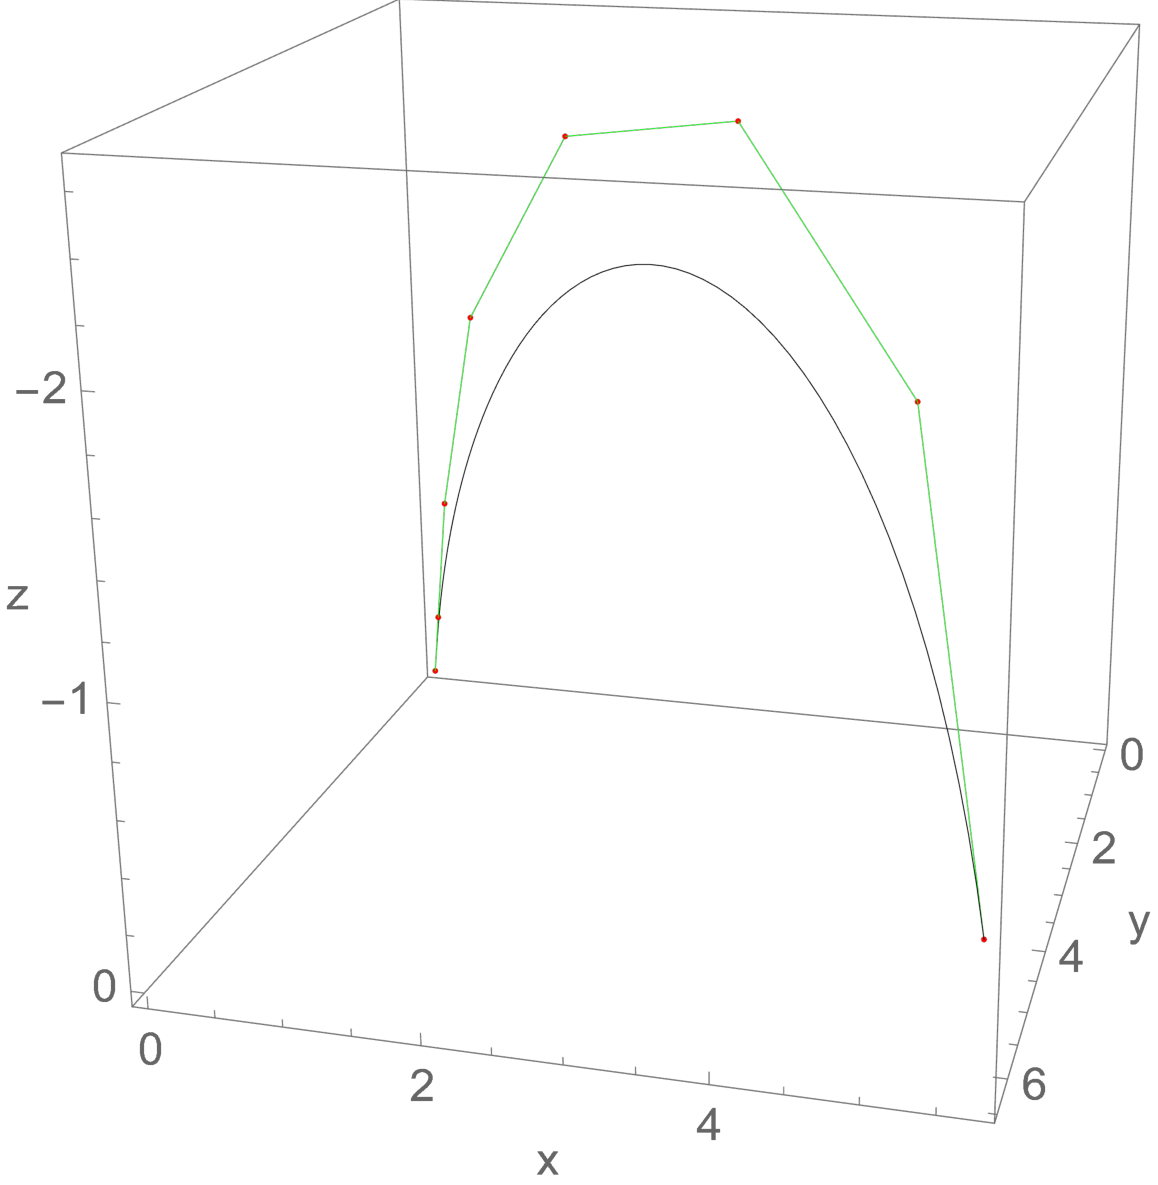
\includegraphics[width=0.5\textwidth]{images/cubic_reparametrization.pdf}
	% \caption[caption za v kazalo]{Dolg caption pod sliko}
	  \caption[Primer vijačne krivulje, pridobljene s kubično reparametrizacijo]{Na sliki je razviden graf vijačne krivulje s pripadajočim kontrolnim poligonom, ki smo jo pridobili s postopkom kubične reparametrizacije parametra $t$ v izrazu \eqref{transformacija}.}
	  \label{fig:cubic_reparametrization}
	\end{figure}
	
	Hodograf je primitiven, saj je $\gcd(x'(t),y'(t),z'(t))=1.$ Parametrična hitrost krivulje je enaka $$\sigma(t)=\lVert\rV'(t)\rVert=3t^6-18t^5+54t^4-54t^3+9t^2+18t+3,$$ razmerje med fleksijsko in torzijsko ukrivljenostjo pa je enako $|\kappa(t)/\tau(t)|=\sqrt{5}/2.$
\end{primer}

\begin{primer}
	\textnormal{ }(Množenje s kvadratičnim polinomom)\textbf{.}
	Videli bomo, kako konstruirati tak tip vijačne krivulje, kot smo ga spoznali v poglavju \ref{mnozenje_kvadraticni_polinom_7}. Za izraz $\zV(t),$ ki predstavlja premico oziroma krožnico v kompleksni ravnini \eqref{transformacija}, izberemo najprej naslednje konstante
	\begin{equation*}
		\aV_0=5\iu,\quad\aV_1=1+\iu,\quad\bV_0=1-\iu,\quad\bV_1=2+5\iu.
	\end{equation*}
	Polinom $\wV$ podamo preko Bernsteinovih koeficientov $\wV_0=1,$ $\wV_1=1+\iu$ in $\wV_2=1.$ Števec in imenovalec izraza $\zV(t)$ množimo z $\wV(t),$ dobimo $\zV(t)=\balpha(t)/\bbeta(t).$ Potem se Bernsteinove koeficiente polinomov $\balpha$ in $\bbeta$ izračuna preko enačb \eqref{mnozenje_kvadraticni_polinom_7_koef1} in \eqref{mnozenje_kvadraticni_polinom_7_koef2}. Enaki so
	\begin{align*}
		\balpha_0&=5\iu,&\balpha_1&=-3+\frac{11}{3}\iu,&\balpha_2&=3\iu,&\balpha_3&=1+\iu,\\
		\bbeta_0&=1-\iu,&\bbeta_1&=2+\frac{5}{3}\iu,&\bbeta_2&=-\frac{5}{3}+\frac{13}{3}\iu,&\bbeta_3&=2+5\iu.
	\end{align*}
	Do kvaternionskega polinoma $\AQ$ se dokopljemo preko zveze $\AQ(t)=\balpha(t)+\kV\bbeta(t).$ S pomočjo Bernsteinovih koeficientov tega polinoma lahko izrazimo kontrolne točke hodografa krivulje oziroma krivulje same, kot smo že opisali v enačbah \eqref{kontrolne_tocke}. Koeficienti so enaki
	\begin{align*}
		\AQ_0&=5\iV-\jV+\kV,&\AQ_2&=3\iV+\frac{13}{3}\jV-\frac{5}{3}\kV,\\
		\AQ_1&=-3+\frac{11}{3}\iV+\frac{5}{3}\jV+2\kV,&\AQ_3&=1+\iV+5\jV+2\kV.
	\end{align*}
	\begin{figure}[h!]
	  \centering
	  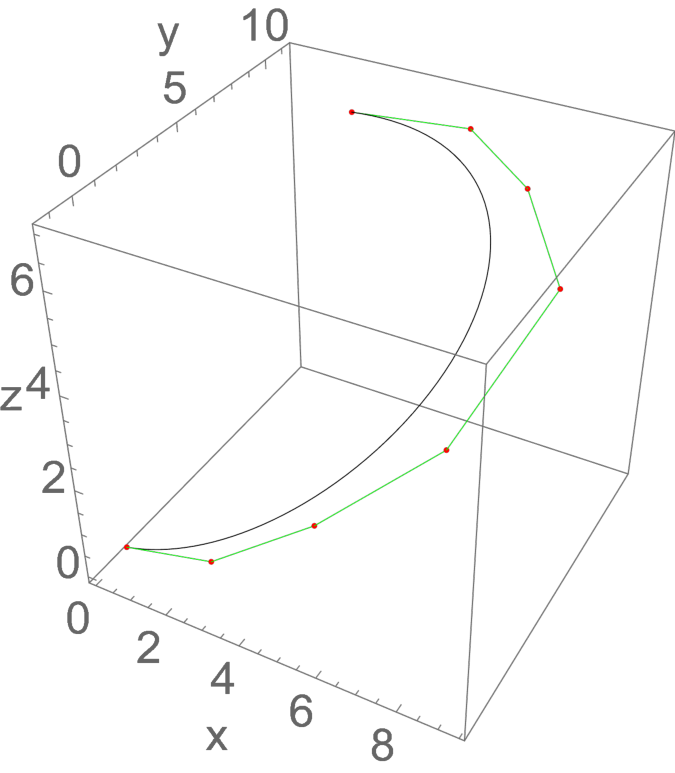
\includegraphics[width=0.5\textwidth]{images/quat_poly_multi.pdf}
	% \caption[caption za v kazalo]{Dolg caption pod sliko}
	  \caption[Primer vijačne krivulje, pridobljene s postopkom množenja z linearnim polinomom]{Na sliki je razviden graf vijačne krivulje s pripadajočim kontrolnim poligonom, ki smo jo pridobili z množenjem števca in imenovalca izraza \eqref{transformacija} s polinomom $\wV.$}
	  \label{fig:quat_poly_multi}
	\end{figure}
	
	Za integracijsko konstanto si izberemo točko $\pV_0=(0,0,0).$ Ostale kontrolne točke krivulje izračunamo preko enačb \eqref{kontrolne_tocke}. Enake so
	\begin{align*}
		\pV_0&=(0,0,0),&\pV_4&=(9.42857, 3.58095, 6.59048),\\
		\pV_1&=(3.28571,-1.42857,1.42857),&\pV_5&=(7.68571, 6.72381, 7.02857),\\
		\pV_2&=(5.85714, -1.19048, 2.95238)&\pV_6&=(5.49524, 9.24762, 7.02857),\\
		\pV_3&=(8.4, -0.104762, 4.7619)&\pV_7&=(1.6381, 11.2476, 6.17143).
	\end{align*}
	Dobimo krivuljo $\rV,$ ki ima komponente enake
	\begin{align*}
		x(t)&=-\frac{80}{7}t^7+\frac{20}{3}t^6+\frac{252}{5}t^5-76t^4+24t^3-15t^2+23t,\\
		y(t)&=-\frac{184}{7}t^7+108t^6-\frac{784}{5}t^5+90t^4-\frac{86}{3}t^3+35t^2-10t,\\
		z(t)&=-\frac{80}{7}t^7+\frac{88}{3}t^6-\frac{72}{5}t^5-16t^4+\frac{20}{3}t^3+2t^2+10t.
	\end{align*}
	Hodograf ni primitiven, saj velja
	\begin{equation*}
		\gcd(x'(t),y'(t),z'(t))=4t^4-8t^3+4t^2+1.
	\end{equation*}
	Parametrična hitrost krivulje je enaka
	\begin{equation*}
		\sigma(t)=\lVert\rV'(t)\rVert=216t^6-632t^5+724t^4-416t^3+162t^2-50t+27,
	\end{equation*}
	razmerje med fleksijsko in torzijsko ukrivljenost pa je enako $|\kappa(t)/\tau(t)|=\sqrt{829}/2.$
\end{primer}

\begin{primer}
	\textnormal{ }(Reparametrizacija in multiplikacija)\textbf{.}
	Tu bomo generirali tak tip krivulje, kot smo ga obravnavali v poglavju \ref{reparametrizacija_multiplikacija}. Podobno kot v prejšnjih primerih, si najprej izberemo konstante
	\begin{equation*}
		\aV_0=1+\iu,\quad\aV_1=1,\quad\bV_0=1-\iu,\quad\bV_1=2.
	\end{equation*}
	Potem izvedemo kvadratično reparametrizacijo preko reparametrizacijske funkcije $f/g,$ ki je določena z naslednjimi Bernsteinovi koeficienti polinomov $f$ in $g:$
	$$(f_0,f_1,f_2)=(1,2,1)\quad\text{in}\quad(g_0,g_1,g_2)=(1,2,2).$$ Nato v ulomku \eqref{transformacija} množimo števec in imenovalec ulomka z linearnim kompleksnim polinomom $\wV,$ ki je podan z Bernsteinovimi koeficienti $(\wV_0,\wV_1)=(1,1+\iu).$ Bernsteinove koeficiente polinomov $\balpha$ in $\bbeta$ lahko tako izračunamo kar preko enačb \eqref{mnozenje_repara_7_koef}. Enaki so
	\begin{align*}
		\balpha_0&=1,&\balpha_1&=\frac{5}{3}+\frac{1}{3}\iu,&\balpha_2&=2+\frac{5}{3}\iu,&\balpha_3&=1+3\iu,\\
		\bbeta_0&=2,&\bbeta_1&=\frac{10}{3}+\frac{2}{3}\iu,&\bbeta_2&=\frac{11}{3}+\frac{7}{3}\iu,&\bbeta_3&=4+2\iu.
	\end{align*}
	Bernsteinove koeficiente kvaternionskega polinoma $\AQ$ izrazimo preko zveze $\AQ_\ell=\balpha_\ell+\kV\bbeta_\ell$ za $\ell=0,1,2,3.$ Enaki so
	\begin{align*}
		\AQ_0&=1+2\kV,&\AQ_2&=2+\frac{5}{3}\iV+\frac{7}{3}\jV+\frac{11}{3}\kV,\\
		\AQ_1&=\frac{5}{3}+\frac{1}{3}\iV+\frac{2}{3}\jV+\frac{10}{3}\kV,&\AQ_3&=1+3\iV+2\jV+4\kV.
	\end{align*}
	Kontrolne točke krivulje $\rV$ izračunamo iz \eqref{kontrolne_tocke}:
	\begin{align*}
		\pV_0&=(0,0,0),&\pV_4&=(-3.5619, 4.92381, 0.314286),\\
		\pV_1&=(-0.428571, 0.571429, 0),&\pV_5&=(-5.28571, 7.57143, 0.980952),\\
		\pV_2&=(-1.14286, 1.52381, 0)&\pV_6&=(-7.04762, 10.7143, 2.6),\\
		\pV_3&=(-2.19048, 2.95238, 0.0571429)&\pV_7&=(-8.47619, 13.5714, 5.45714).
	\end{align*}
	S tem je krivulja $\rV$ določena. Njene komponente so enake
	\begin{align*}
		x(t)&=-\frac{8}{7}t^7+\frac{10}{3}t^6-2t^5+2t^4-\frac{5}{3}t^3-6t^2-3t,\\
		y(t)&=\frac{4}{7}t^7-\frac{10}{3}t^6+2t^5-t^4+\frac{10}{3}t^3+8t^2+4t,\\
		z(t)&=-\frac{8}{7}t^7+2t^6-\frac{2}{5}t^5+3t^4+2t^3.
	\end{align*}
	Hodograf ni primitiven, saj je $\gcd(x'(t),y'(t),z'(t))=t^2+1.$ Parametrična hitrost krivulje je tu enaka
	\begin{equation*}
		\sigma(t)=\lVert\rV'(t)\rVert=12t^6-28t^5+18t^4-8t^3+11t^2+20t+5,
	\end{equation*}
	razmerje med fleksijsko in torzijsko ukrivljenost pa je enako $|\kappa(t)/\tau(t)|=\sqrt{10}.$
	\begin{figure}[h!]
	  \centering
	  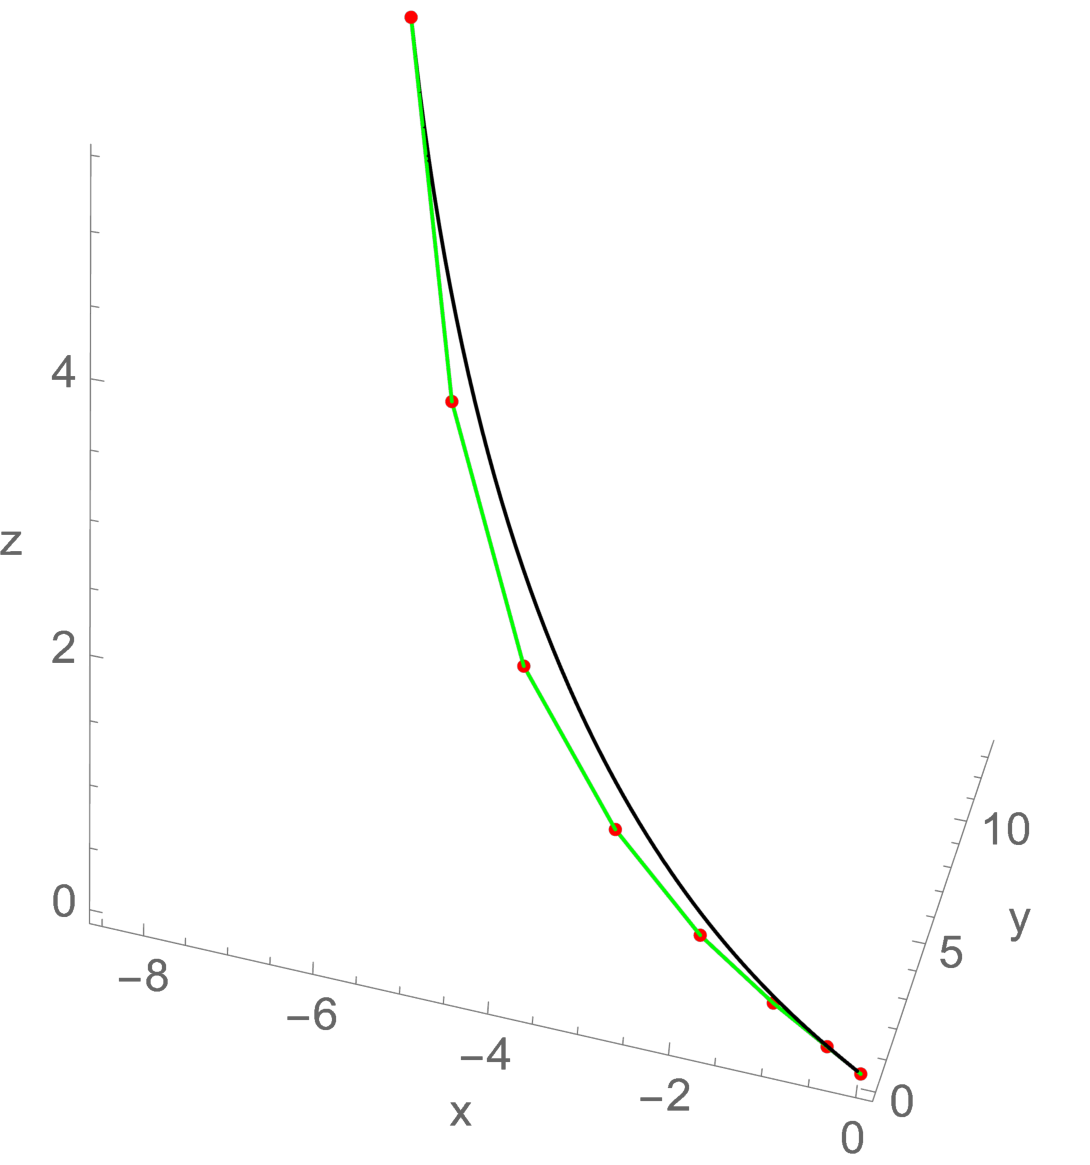
\includegraphics[width=0.5\textwidth]{images/reparametrization_multi.pdf}
	% \caption[caption za v kazalo]{Dolg caption pod sliko}
	  \caption[Primer vijačne krivulje, pridobljene s postopkom reparametrizacije in multiplikacije]{Na sliki je razviden graf vijačne krivulje s pripadajočim kontrolnim poligonom, ki smo jo pridobili s postopkom reparametrizacije in multiplikacije}
	  \label{fig:reparametrization_multi}
	\end{figure}
\end{primer}

Sedaj bomo obravnavali še razne primere konstrukcij DPH krivulj za različne stopnje polinomov $h$ in $\wV,$ kot smo jih analizirali v poglavju \ref{poglavje_dvojnePHkrivulje7}. Obenem bomo še uporabili kriterije za ločevanje med vijačnimi in nevijačnimi krivuljami, kot smo jih razvili v poglavju \ref{poglavje_nevijacne}.

\begin{primer}
	\label{primer_h0w2_vijacna}
	\textnormal{ }(Vijačna, $\st(h)=0,\st(\wV)=2$)\textbf{.}
	Ogledali si bomo primer krivulje takega tipa, kot smo ga obravnavali v poglavju \ref{klasifikacija_h0w2}. Najprej si izberemo polinoma $h$ in $\wV$ z naslednjimi Bernsteinovimi koeficienti
	$$h_0=1,\quad\wV_0=1,\quad\wV_1=1+\iu,\quad\wV_2=\iu.$$
	Izberemo si še vrednosti koeficientov $\balpha_0=1,\balpha_1=2\iu$ in $\bbeta_0=\iu,$ ter drugo rešitev za $\zV$ v \eqref{st7h0w2}. Nato lahko rešimo sistem enačb \eqref{sistem_st7h0w2}. Sistem lahko rešimo kar s pomočjo programa \emph{Mathematica}. Ko to naredimo, dobimo vse Bernsteinove koeficiente za polinoma $\balpha$ in $\bbeta:$
	\begin{align*}
		\balpha_0&=1,&\balpha_1&=2\iu,&\balpha_2&=-4+\frac{5}{3}\iu,&\balpha_3&=-4-2\iu,\\
		\bbeta_0&=\iu,&\bbeta_1&=-\frac{5}{3},&\bbeta_2&=-1-\frac{10}{3}\iu,&\bbeta_3&=2-3\iu.
	\end{align*}
	S pomočjo teh koeficientov lahko izračunamo tudi Bernsteinove koeficiente kvaternionskega polinoma $\AQ,$ ki so enaki
	\begin{align*}
		\AQ_0&=1+\jV,&\AQ_2&=-4+\frac{5}{3}\iV-\frac{10}{3}\jV-\kV,\\
		\AQ_1&=2\iV-\frac{5}{3}\kV,&\AQ_3&=-4-2\iV-3\jV+2\kV.
	\end{align*}
	\begin{figure}[h]
	  \centering
	  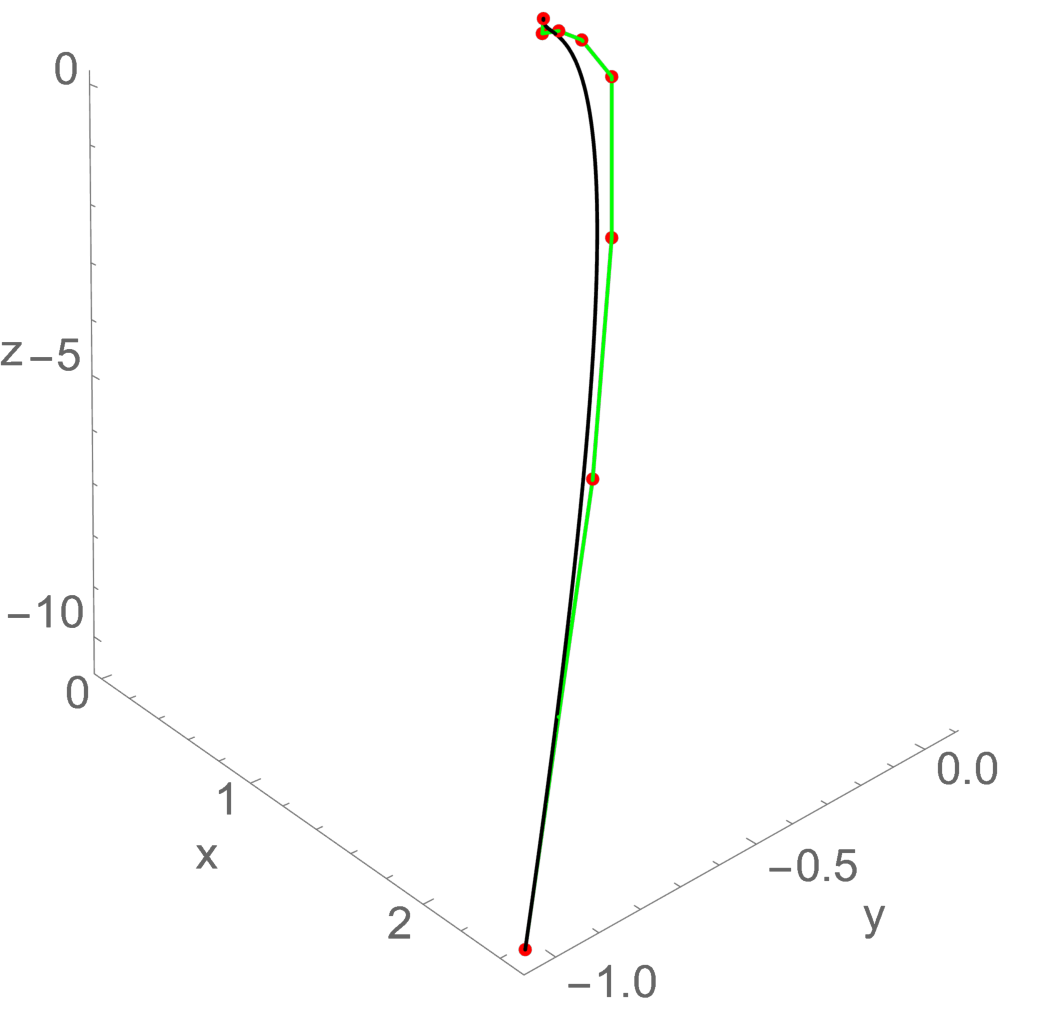
\includegraphics[width=0.5\textwidth]{images/h0w2_vijacna.pdf}
	% \caption[caption za v kazalo]{Dolg caption pod sliko}
	  \caption[Primer vijačne krivulje ($\st(h)=0,$ $\st(\wV)=2$)]{Na sliki je razviden graf vijačne krivulje s pripadajočim kontrolnim poligonom, za katero velja $\st(h)=0$ in $\st(\wV)=2.$}
	  \label{fig:h0w2_vijacna}
	\end{figure}
	Ob upoštevanju zvez \eqref{kontrolne_tocke} so kontrolne točke krivulje $\rV$ enake
	\begin{align*}
		\pV_0&=(0,0,0),&\pV_4&=(0.266667, 0.0857143, -0.952381),\\
		\pV_1&=(0, 0, -0.285714),&\pV_5&=(0.8, -0.142857, -3.10476),\\
		\pV_2&=(0, 0.047619, -0.285714)&\pV_6&=(1.46667, -0.47619, -5.9619),\\
		\pV_3&=(0.0666667, 0.0857143, -0.438095)&\pV_7&=(2.46667, -1.04762, -10.5333).
	\end{align*}
	Komponente krivulje $\rV$ so potem enake
	\begin{align*}
		x(t)&=2t^7-\frac{14}{3}t^6+\frac{14}{5}t^5+\frac{7}{3}t^3,\\
		y(t)&=-\frac{12}{7}t^7+\frac{14}{3}t^6-4t^5+t^4-2t^3+t^2,\\
		z(t)&=-12t^7+32t^6-\frac{136}{5}t^5+8t^4-\frac{46}{3}t^3+6t^2-2t.
	\end{align*}
	Hodograf ni primitiven, saj je $\gcd(x'(t),y'(t),z'(t))=2t^4-4t^3+2t^2+1.$ Parametrična hitrost krivulje je enaka
	\begin{equation*}
		\sigma(t)=\lVert\rV'(t)\rVert=86t^6-196t^5+138t^4-32t^3+47t^2-12t+2,
	\end{equation*}
	razmerje med fleksijsko in torzijsko ukrivljenost pa je enako $|\kappa(t)/\tau(t)|=1/7.$ Po Lancretovem izreku \ref{lancret} velja, da je ta krivulja vijačna.
\end{primer}

\begin{primer}
	\label{primer_h0w2_nevijacna}
	\textnormal{ }(Nevijačna, $\st(h)=0,\st(\wV)=2$)\textbf{.}
	Sedaj si bomo ogledali še primer nevijačne krivulje, kjer je $\st(h)=0$ in $\st(\wV)=2.$ Izberemo si ista polinoma $h$ in $\wV$ in iste koeficiente $\balpha_0,\balpha_1$ in $\bbeta_0,$ kot smo jih izbrali v primeru \ref{primer_h0w2_vijacna}, le da vzamemo prvi izraz za $\zV$ namesto drugega v \eqref{st7h0w2}. Potem rešimo sistem enačb \eqref{sistem_st7h0w2} in dobimo Bernsteinove koeficiente za polinoma $\balpha$ in $\bbeta:$
	\begin{align*}
		\balpha_0&=1,&\balpha_1&=2\iu,&\balpha_2&=-4+3\iu,&\balpha_3&=-12-2\iu,\\
		\bbeta_0&=\iu,&\bbeta_1&=-\frac{5}{3},&\bbeta_2&=-\frac{7}{3}-\frac{10}{3}\iu,&\bbeta_3&=2-\frac{29}{3}\iu.
	\end{align*}
	Bernsteinovi koeficienti kvaternionskega polinoma $\AQ$ so potem enaki
	\begin{align*}
		\AQ_0&=1+\jV,&\AQ_2&=-4+3\iV-\frac{10}{3}\jV-\frac{7}{3}\kV,\\
		\AQ_1&=2\iV-\frac{5}{3}\kV,&\AQ_3&=-12-2\iV-\frac{29}{3}\jV+2\kV.
	\end{align*}
	Kontrolne točke krivulje $\rV$ so enake
	\begin{align*}
		\pV_0&=(0,0,0),&\pV_4&=(0.304762, 0.0857143, -1.37143),\\
		\pV_1&=(0, 0, -0.285714),&\pV_5&=(0.990476, 0.00952381, -4.4381),\\
		\pV_2&=(0, 0.047619, -0.285714)&\pV_6&=(3.05397, -0.32381, -14.1524),\\
		\pV_3&=(0.0666667, 0.0857143, -0.438095)&\pV_7&=(10.2762, -1.65714, -48.4381).
	\end{align*}
	S kontrolni točkami krivulje $\rV$ so določene tudi komponente krivulje $\rV,$ ki so enake
	\begin{align*}
		x(t)&=\frac{86}{63}t^7+\frac{22}{9}t^6+\frac{14}{5}t^5+\frac{4}{3}t^4+\frac{7}{3}t^3,\\
		y(t)&=-\frac{4}{21}t^7-\frac{2}{3}t^6-\frac{4}{5}t^5+t^4-2t^3+t^2,\\
		z(t)&=-\frac{124}{21}t^7-\frac{40}{3}t^6-\frac{56}{5}t^5-\frac{20}{3}t^4-\frac{46}{3}t^3+6t^2-2t.
	\end{align*}
	Hodograf je primitiven, saj je $\gcd(x'(t),y'(t),z'(t))=1/9,$ parametrična hitrost krivulje pa je enaka
	\begin{equation*}
		\sigma(t)=\lVert\rV'(t)\rVert=\frac{382}{9}t^6+\frac{244}{3}t^5+58t^4+\frac{80}{3}t^3+47t^2-12t+2,
	\end{equation*}
	razmerje med fleksijsko in torzijsko ukrivljenost pa je enako $$\left|\frac{\kappa(t)}{\tau(t)}\right|=\left|\frac{9(2t^4-4t^3+2t^2+1)^2}{460t^8-1840t^7-296t^6-2688t^5+1272t^4+624t^3-180t^2+144t+63}\right|.$$ Po Lancretovem izreku \ref{lancret} vidimo, da je ta krivulja nevijačna.
	
	To lahko preverimo tudi drugače. Polinom $\wV$ ima ničli $\btau_1,\btau_2=\frac{1}{2}(1\pm\sqrt{2}+\iu).$ Ti ničli nista obe realni, in nista par konjugiranih si kompleksnih števil. Z nekaj osnovnega računanja lahko preverimo, da se da polinoma $\balpha$ in $\bbeta$ zapisati v obliki \eqref{polinoma_h0w2} s koeficienti
	\begin{align*}
		\aV_1&=\frac{1}{2}\big(\sqrt{2}-1+(4\sqrt{2}-5)\iu\big),&\bV_1&=\frac{1}{3}\big(6-5\sqrt{2}+(\sqrt{2}-1)\iu\big),\\
		\aV_2&=-\frac{1}{2}\big(\sqrt{2}+1+(4\sqrt{2}+5)\iu\big),&\bV_2&=\frac{1}{3}\big(6+5\sqrt{2}-(\sqrt{2}+1)\iu\big).
	\end{align*}
	Ker velja $\aV_1\bV_2-\aV_2\bV_1=-\frac{\sqrt{2}}{3}\iu\neq 0,$ so potem pogoji za trditev \ref{locevanje_trditev_h0w2} izpolnjeni in je krivulja tudi po tej trditvi res nevijačna.
	\begin{figure}[h]
	  \centering
	  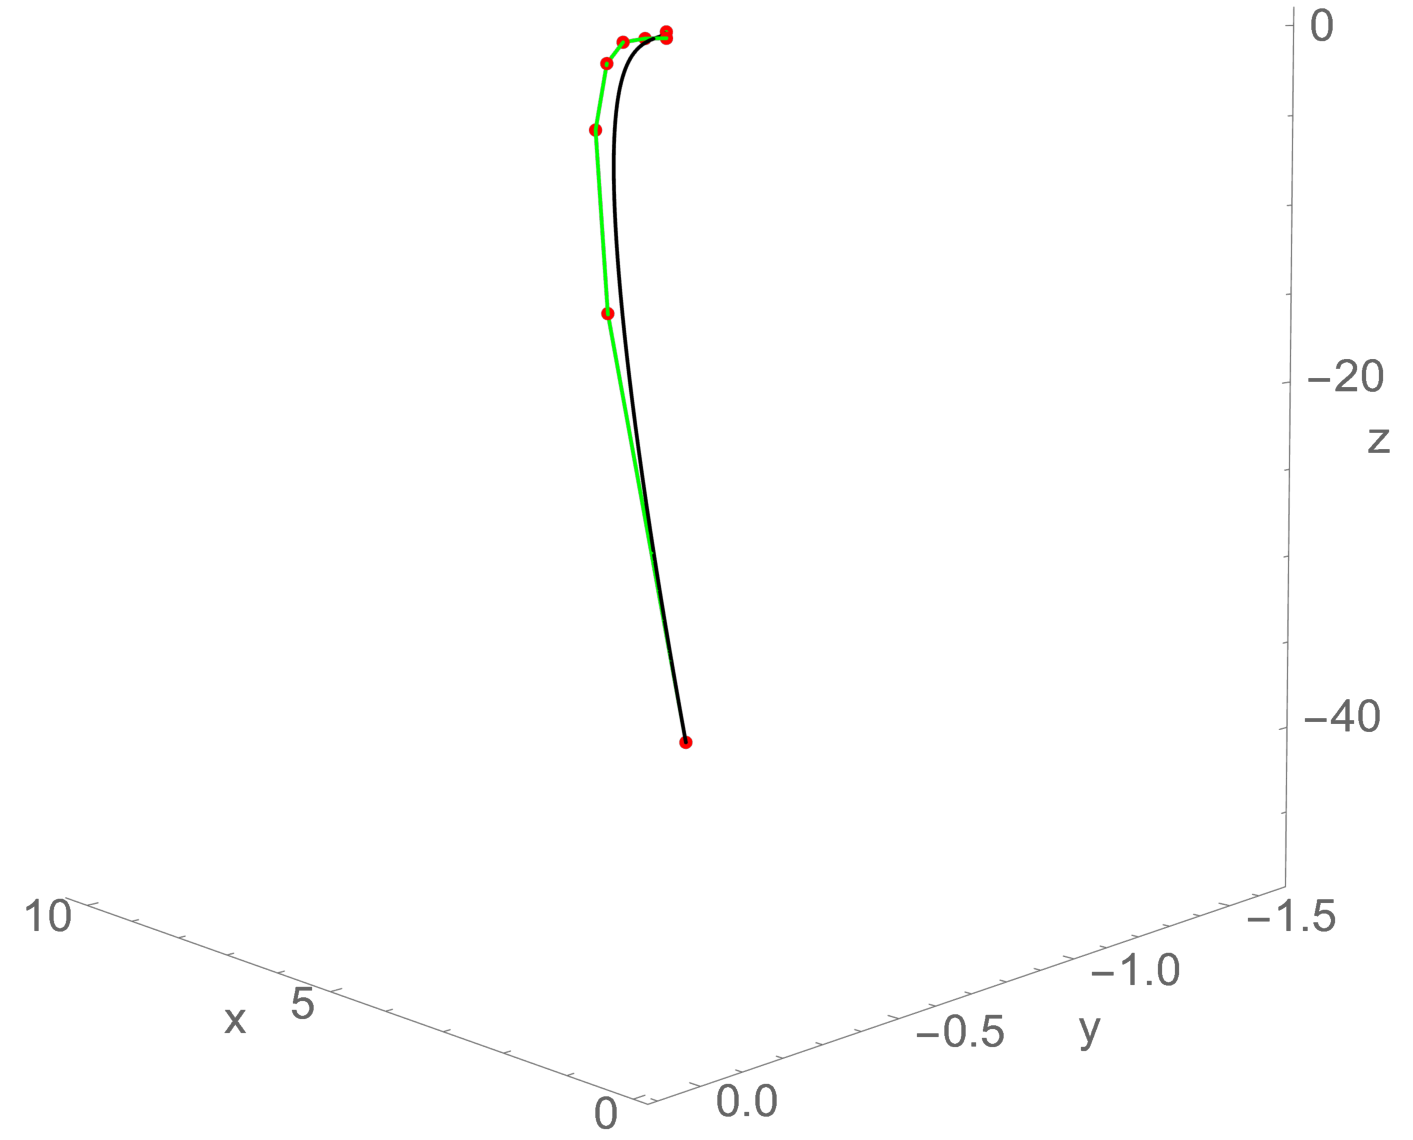
\includegraphics[width=0.5\textwidth]{images/h0w2_nevijacna.pdf}
	% \caption[caption za v kazalo]{Dolg caption pod sliko}
	  \caption[Primer nevijačne krivulje ($\st(h)=0,$ $\st(\wV)=2$)]{Na sliki je razviden graf nevijačne krivulje s pripadajočim kontrolnim poligonom, za katero velja $\st(h)=0$ in $\st(\wV)=2.$}
	  \label{fig:h0w2_nevijacna}
	\end{figure}
\end{primer}

\begin{primer}
	\label{primer_h2w1_vijacna}
	\textnormal{ }(Vijačna, $\st(h)=2,\st(\wV)=1$)\textbf{.}
	Sedaj je na vrsti primer krivulje takega tipa, kot smo ga obravnavali v poglavju \ref{klasifikacija_h2w1}. Izberimo si naslednje Bernsteinove koeficiente za polinoma $h$ in $\wV:$
	$$h_0=1,\quad h_1=2,\quad h_2=1,\quad\wV_0=\iu,\quad\wV_1=1.$$
	Podobno kot v prejšnjih primerih si izberemo vrednosti $\balpha_0=1,$ $\balpha_1=1,$ $\bbeta_=-1$ ter drugo rešitev za $\zV$ v \eqref{st7h2w1}. Sedaj imamo vse potrebno, da lahko rešimo sistem \eqref{sistem_st7h0w2} in da dobimo Bernsteinove koeficiente polinomov $\balpha$ in $\bbeta:$
	\begin{align*}
		\balpha_0&=1,&\balpha_1&=1,&\balpha_2&=2-\frac{1}{3}\iu,&\balpha_3&=2-5\iu,\\
		\bbeta_0&=-1,&\bbeta_1&=-\frac{4}{3},&\bbeta_2&=-\frac{8}{3}+\frac{2}{3}\iu,&\bbeta_3&=-2+7\iu.
	\end{align*}
	Kvaternionski polinom $\AQ$ ima potem naslednje Bernsteinove koeficiente
	\begin{align*}
		\AQ_0&=1-\kV,&\AQ_2&=2-\frac{1}{3}\iV+\frac{2}{3}\jV-\frac{8}{3}\kV,\\
		\AQ_1&=1-\frac{4}{3}\kV,&\AQ_3&=2-5\iV+7\jV-2\kV.
	\end{align*}
	Kontrolne točke krivulje $\rV$ so potemtakem enake
	\begin{align*}
		\pV_0&=(0,0,0),&\pV_4&=(-0.35238, -1.8571, -0.076191),\\
		\pV_1&=(0, -0.28571, 0),&\pV_5&=(-0.68571, -3.0762, -0.17143),\\
		\pV_2&=(-0.04762, -0.61905, 0)&\pV_6&=(-1.3048, -5.2191, -0.36191),\\
		\pV_3&=(-0.15238, -1.1143, -0.019048)&\pV_7&=(-4.7333, -16.362, -1.5048).
	\end{align*}
	\begin{figure}[h]
	  \centering
	  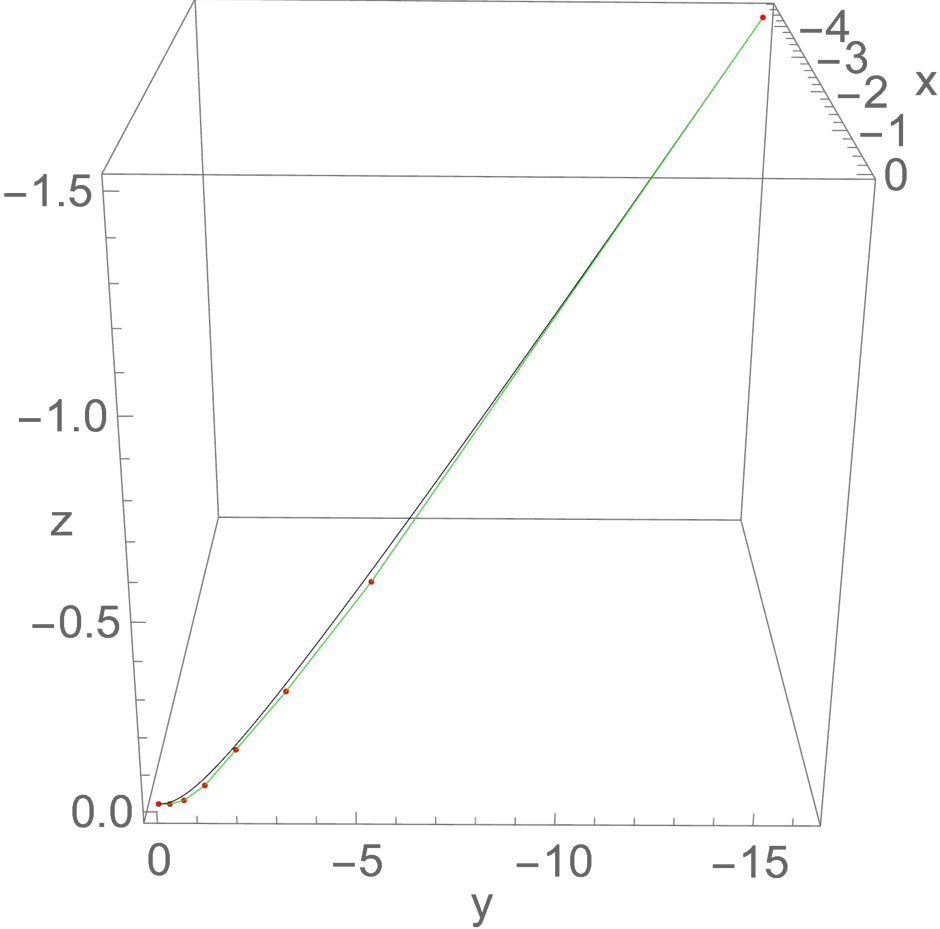
\includegraphics[width=0.45\textwidth]{images/h2w1_vijacna.pdf}
	% \caption[caption za v kazalo]{Dolg caption pod sliko}
	  \caption[Primer vijačne krivulje ($\st(h)=2,$ $\st(\wV)=1$)]{Na sliki je razviden graf vijačne krivulje s pripadajočim kontrolnim poligonom, za katero velja $\st(h)=2$ in $\st(\wV)=1.$}
	  \label{fig:h2w1_vijacna}
	\end{figure}

	Komponente krivulje $\rV$ so tako enake
	\begin{align*}
		x(t)&=-2t^7-t^6+\frac{3}{5}t^5-t^4-\frac{1}{3}t^3-t^2,\\
		y(t)&=-\frac{52}{7}t^7+\frac{2}{3}t^6-\frac{18}{5}t^5+t^4-4t^3-t^2-2t,\\
		z(t)&=-\frac{4}{7}t^7-\frac{2}{3}t^6+\frac{2}{5}t^5-\frac{2}{3}t^3.
	\end{align*}
	Hodograf ni primitiven, saj je $\gcd(x'(t),y'(t),z'(t))=2t^2-2t+1.$ Parametrična hitrost krivulje je enaka
	\begin{equation*}
		\sigma(t)=\lVert\rV'(t)\rVert=54t^6-2t^5+17t^4-4t^3+13t^2+2t+2,
	\end{equation*}
	razmerje med fleksijsko in torzijsko ukrivljenost pa je enako $|\kappa(t)/\tau(t)|=1/2.$ Po Lancretovem izreku \ref{lancret} velja, da je ta krivulja vijačna.
	
	Ni težko videti, da je $\bgamma(t)=\gcd(\balpha(t),\bbeta(t))=(1+\iu)t-1.$ Torej je $r=\st(\bgamma)=1.$ Po trditvi \ref{locevanje_h2w1_trditev1} lahko še lažje preverimo, da je ta krivulja res vijačna.
\end{primer}

\begin{primer}
	\label{primer_h2w1_nevijacna}
	\textnormal{ }(Nevijačna, $\st(h)=2,\st(\wV)=1$)\textbf{.}
	Sedaj si bomo ogledali še primer nevijačne krivulje, kjer je $\st(h)=2$ in $\st(\wV)=1.$ Izberemo si ista polinoma $h$ in $\wV$ in iste koeficiente $\balpha_0,\balpha_1$ in $\bbeta_0,$ kot smo jih izbrali v primeru \ref{primer_h2w1_vijacna}, le da vzamemo prvi izraz za $\zV$ namesto drugega v \eqref{st7h0w2}. Nato še rešimo sistem enačb \eqref{sistem_st7h0w2} in dobimo Bernsteinove koeficiente za polinoma $\balpha$ in $\bbeta:$
	\begin{align*}
	\balpha_0&=1,&\balpha_1&=1,&\balpha_2&=2+\iu,&\balpha_3&=2-\iu,\\
		\bbeta_0&=-1,&\bbeta_1&=-\frac{4}{3},&\bbeta_2&=-\frac{8}{3}-\frac{2}{3}\iu,&\bbeta_3&=-2+\frac{5}{3}\iu.
	\end{align*}
	Bernsteinovi koeficienti kvaternionskega polinoma $\AQ$ so tako enaki
	\begin{align*}
		\AQ_0&=1-\kV,&\AQ_2&=2+\iV-\frac{2}{3}\jV-\frac{8}{3}\kV,\\
		\AQ_1&=1-\frac{4}{3}\kV,&\AQ_3&=2-\iV+\frac{5}{3}\jV-2\kV.
	\end{align*}
	Preko enačb \eqref{kontrolne_tocke} izračunamo, da so kontrolne točke krivulje $\rV$ enake
	\begin{align*}
		\pV_0&=(0,0,0),&\pV_4&=(-0.352381, -1.85714, -0.114286),\\
		\pV_1&=(0, -0.285714, 0),&\pV_5&=(-0.609524, -3.15238, -0.361905),\\
		\pV_2&=(-0.047619, -0.619048, 0)&\pV_6&=(-0.784127, -4.15238, -0.552381),\\
		\pV_3&=(-0.152381, -1.11429, -0.0190476)&\pV_7&=(-1.0381, -5.77143, -0.933333).
	\end{align*}
	S kontrolni točkami krivulje $\rV$ imamo določene tudi komponente krivulje $\rV,$ ki so enake
	\begin{align*}
		x(t)&=-\frac{22}{63}t^7-\frac{5}{9}t^6+\frac{11}{5}t^5-t^4-\frac{1}{3}t^3-t^2,\\
		y(t)&=-\frac{124}{21}t^7+\frac{34}{3}t^6-\frac{26}{5}t^5+t^4-4t^3-t^2-2t,\\
		z(t)&=-\frac{4}{3}t^7+2t^6+\frac{2}{5}t^5-\frac{4}{3}t^4-\frac{2}{3}t^3.
	\end{align*}
	Hodograf je primitiven, saj je $\gcd(x'(t),y'(t),z'(t))=1/9,$ parametrična hitrost krivulje pa je enaka
	\begin{equation*}
		\sigma(t)=\lVert\rV'(t)\rVert=\frac{382}{9}t^6-\frac{206}{3}t^5+25t^4-4t^3+13t^2+2t+2,
	\end{equation*}
	razmerje med fleksijsko in torzijsko ukrivljenost pa je enako $$\left|\frac{\kappa(t)}{\tau(t)}\right|=\left|\frac{9(2t^2-2t-1)(2t^2-2t+1)^2}{2(92t^6-276t^5-60t^4+228t^3-126t^2+54t+9)}\right|.$$ Po Lancretovem izreku \ref{lancret} je ta krivulja nevijačna.
	
	Lažje lahko to preverimo s pomočjo trditve \ref{locevanje_h2w1_trditev2}. Ni težko videti, da sta si polinoma $\balpha$ in $\bbeta$ tuja, torej je $r=\st(\bgamma)=\st(\gcd(\balpha,\bbeta))=0.$ Po trditvi \ref{locevanje_h2w1_trditev2} je naša krivulja nevijačna.
	\begin{figure}[h]
	  \centering
	  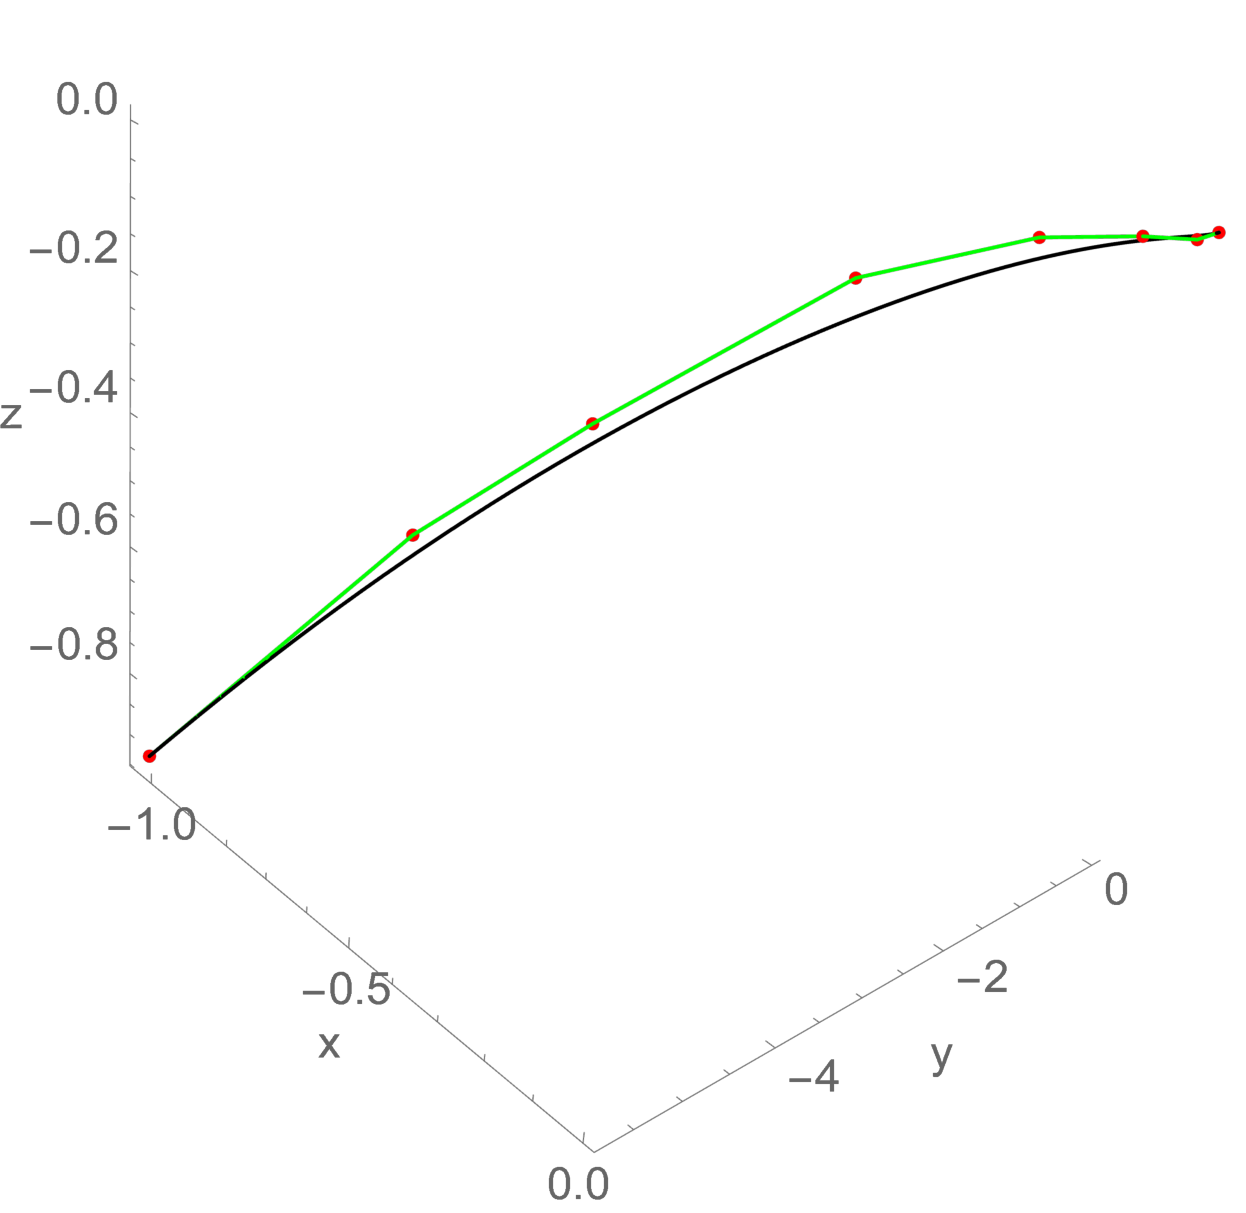
\includegraphics[width=0.5\textwidth]{images/h2w1_nevijacna.pdf}
	% \caption[caption za v kazalo]{Dolg caption pod sliko}
	  \caption[Primer nevijačne krivulje ($\st(h)=2,$ $\st(\wV)=1$)]{Na sliki je razviden graf nevijačne krivulje s pripadajočim kontrolnim poligonom, za katero velja $\st(h)=2$ in $\st(\wV)=1.$}
	  \label{fig:h2w1_nevijacna}
	\end{figure}
\end{primer}

\begin{primer}
	\textnormal{ }(Vijačna, $\st(h)=4,$ $\st(\wV)=0$)\textbf{.}
	Konstruirali bomo krivuljo takega tipa, kot smo ga analizirali v poglavju \ref{klasifikacija_h4w0}. Za začetek si izberemo naslednja polinoma $h$ in $\wV,$ izražena v Bernsteinovi bazi z izbiro koeficientov
	\begin{equation*}
		h_0=-1,\quad h_1=2,\quad h_2=3,\quad h_3=4,\quad h_4=-5,\quad \wV_0=1.
	\end{equation*}
	Vidimo, da je količina $\Delta=9h_2^2+3h_0h_4-12h_1h_4=0$ nenegativna in po trditvi \ref{trditev_locevanje_h4w0} sledi, da je krivulja, ki jo generiramo, vijačna. Prosto si izberemo še vrednosti koeficientov $\balpha_0=1,$ $\balpha_1=1-\iu$ in $\bbeta_0=-1-\iu.$ Nato rešimo sistem enačb \eqref{sistem_st7h4w0} in pri tem upoštevamo rešitev, ki ima pozitivni predznak pri korenu v $\zV=\balpha_1\bbeta_2-\balpha_2\bbeta_1$ v enačbi \eqref{st7h4w0}. Tako dobimo naslednje Bernsteinove koeficiente za polinoma $\balpha$ in $\bbeta:$
	\begin{align*}
		\balpha_0&=1,&\balpha_1&=1-\iu,&\balpha_2&=-1+4\iu,&\balpha_3&=-1+9\iu,\\
		\bbeta_0&=-1+\iu,&\bbeta_1&=-\frac{1}{3}+2\iu,&\bbeta_2&=-\frac{5}{3}-5\iu,&\bbeta_3&=-5-10\iu.
	\end{align*}
	Z relacijo $\AQ(t)=\balpha(t)+\kV\bbeta(t)$ pridobimo kvaternionski zapis, preko katerega izrazimo zapis hodografa krivulje. Bernsteinovi koeficienti kvaternionskega polinoma $\AQ$ so enaki
	\begin{align*}
		\AQ_0&=1+\jV-\kV,&\AQ_2&=-1+4\iV-5\jV-\frac{5}{3}\kV,\\
		\AQ_1&=1-\iV+2\jV-\frac{1}{3}\kV,&\AQ_3&=-1+9\iV-10\jV-5\kV.
	\end{align*}
	Za integracijsko konstanto si kot ponavadi izberemo točko $\pV_0=(0,0,0).$ Ostale kontrolne točke krivulje izračunamo preko enačb \eqref{kontrolne_tocke}. Enake so
	\begin{align*}
		\pV_0&=(0,0,0),&\pV_4&=(0.247619, 0.742857, 0.228571),\\
		\pV_1&=(-0.142857, -0.285714, -0.285714),&\pV_5&=(-0.2, -1.06667, -0.971429),\\
		\pV_2&=(-0.333333, -0.619048, -0.571429)&\pV_6&=(-3.24762, -12.2571, -8.11429),\\
		\pV_3&=(-0.380952, -0.828571, -0.742857)&\pV_7&=(-9.39048, -36.5429, -23.8286).
	\end{align*}
	\begin{figure}[h]
	  \centering
	  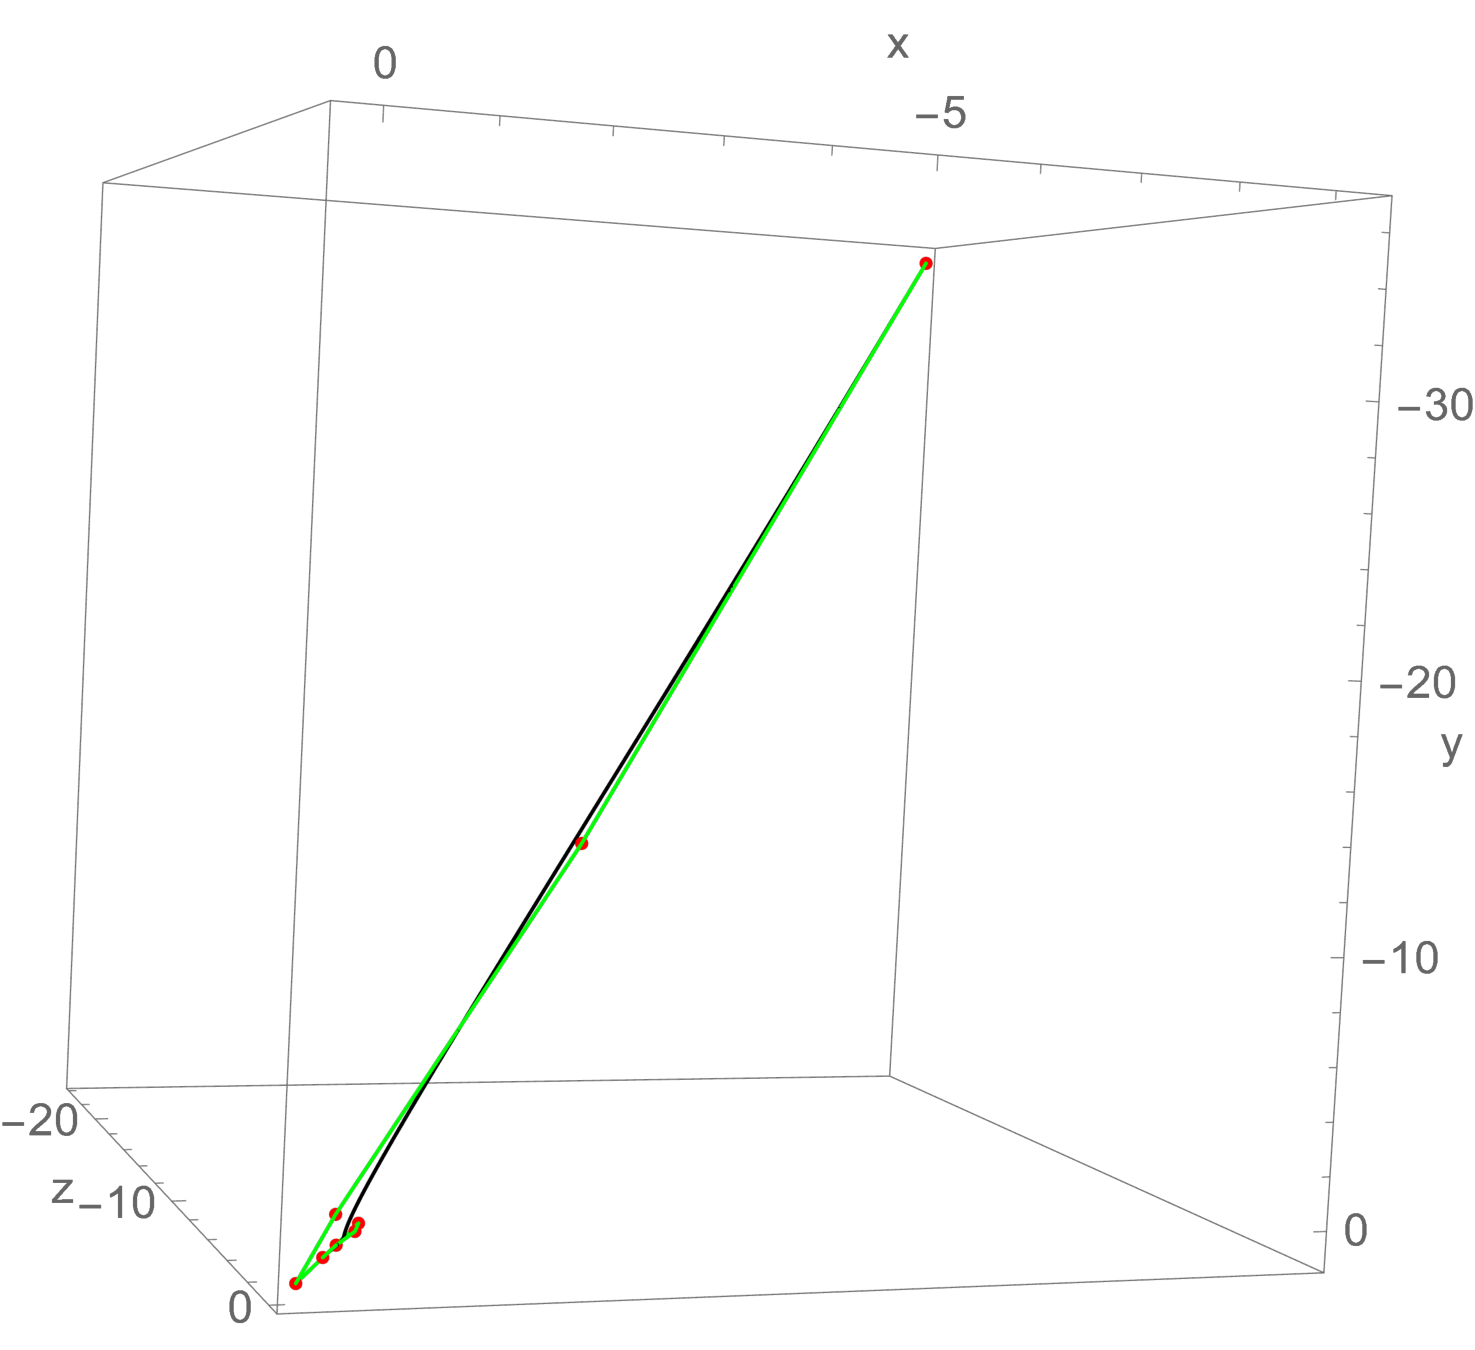
\includegraphics[width=0.5\textwidth]{images/h4w0_vijacna.pdf}
	% \caption[caption za v kazalo]{Dolg caption pod sliko}
	  \caption[Primer vijačne krivulje ($\st(h)=4,$ $\st(\wV)=0$)]{Na sliki je razviden graf vijačne krivulje s pripadajočim kontrolnim poligonom, za katero velja $\st(h)=4$ in $\st(\wV)=0.$}
	  \label{fig:h4w0_vijacna}
	\end{figure}
	
	S tem dobimo krivuljo $\rV,$ ki ima komponente enake
	\begin{align*}
		x(t)&=-\frac{48}{7}t^7+36t^6-\frac{276}{5}t^5+12t^4+\frac{20}{3}t^3-t^2-t,\\
		y(t)&=-\frac{120}{7}t^7+100t^6-\frac{872}{5}t^5+52t^4+6t^3-t^2-2t,\\
		z(t)&=-\frac{80}{7}t^7+64t^6-\frac{552}{5}t^5+32t^4+4t^3-2t.
	\end{align*}
	Hodograf je primitiven, saj velja $\gcd(x'(t),y'(t),z'(t))=1.$ Parametrična hitrost krivulje $\sigma(t)$ je enaka
	\begin{equation*}
		\sigma(t)=\lVert\rV'(t)\rVert=152t^6-744t^5+1068t^4-248t^3-26t^2+2t+3.
	\end{equation*}
	Razmerje med fleksijsko in torzijsko ukrivljenostjo je enako $|\kappa(t)/\tau(t)|=1/8,$ kar je identično enako konstanti. Tudi po Lancretovem izreku \ref{lancret} lahko preverimo, da je taka krivulja res nevijačna.
\end{primer}

\begin{primer}
	\textnormal{ }(Nevijačna, $\st(h)=4,$ $\st(\wV)=0$)\textbf{.}
	Sedaj si bomo še ogledali nevijačno krivuljo, kjer je $\st(h)=4$ in $\st(\wV)=0.$ Izberemo si naslednja polinoma $h$ in $\wV,$ izražena v Bernsteinovi bazi z izbiro koeficientov
	\begin{equation*}
		h_0=1,\quad h_1=2,\quad h_2=2,\quad h_3=2,\quad h_4=1,\quad \wV_0=1.
	\end{equation*}
	Tokrat je količina $\Delta=9h_2^2+3h_0h_4-12h_1h_4=-9$ negativna in po trditvi \ref{trditev_locevanje_h4w0} sledi, da je krivulja, ki jo generiramo, nevijačna. Podobno kot v prejšnjih primerih si prosto izberemo še vrednosti koeficientov $\balpha_0=1,$ $\balpha_1=1$ in $\bbeta_0=-1.$ Nato rešimo sistem enačb \eqref{sistem_st7h4w0} in pri tem upoštevamo rešitev, ki ima negativni predznak pri korenu v $\zV=\balpha_1\bbeta_2-\balpha_2\bbeta_1$ v enačbi \eqref{st7h4w0}. Dobimo naslednje Bernsteinove koeficiente za polinoma $\balpha$ in $\bbeta:$
	\begin{align*}
		\balpha_0&=1,&\balpha_1&=1,&\balpha_2&=2+\iu,&\balpha_3&=2+3\iu,\\
		\bbeta_0&=-1,&\bbeta_1&=-\frac{2}{3},&\bbeta_2&=-\frac{2}{3}-\iu,&\bbeta_3&=-2\iu.
	\end{align*}
	Bernsteinovi koeficienti kvaternionskega polinoma $\AQ$ so enaki
	\begin{equation*}
		\AQ_0=1-\kV,\quad\AQ_1=1-\frac{2}{3}\kV,\quad\AQ_2=2+\iV-\jV-\frac{2}{3}\kV,\quad\AQ_3=2+3\iV-2\jV.
	\end{equation*}
	\begin{figure}[h]
	  \centering
	  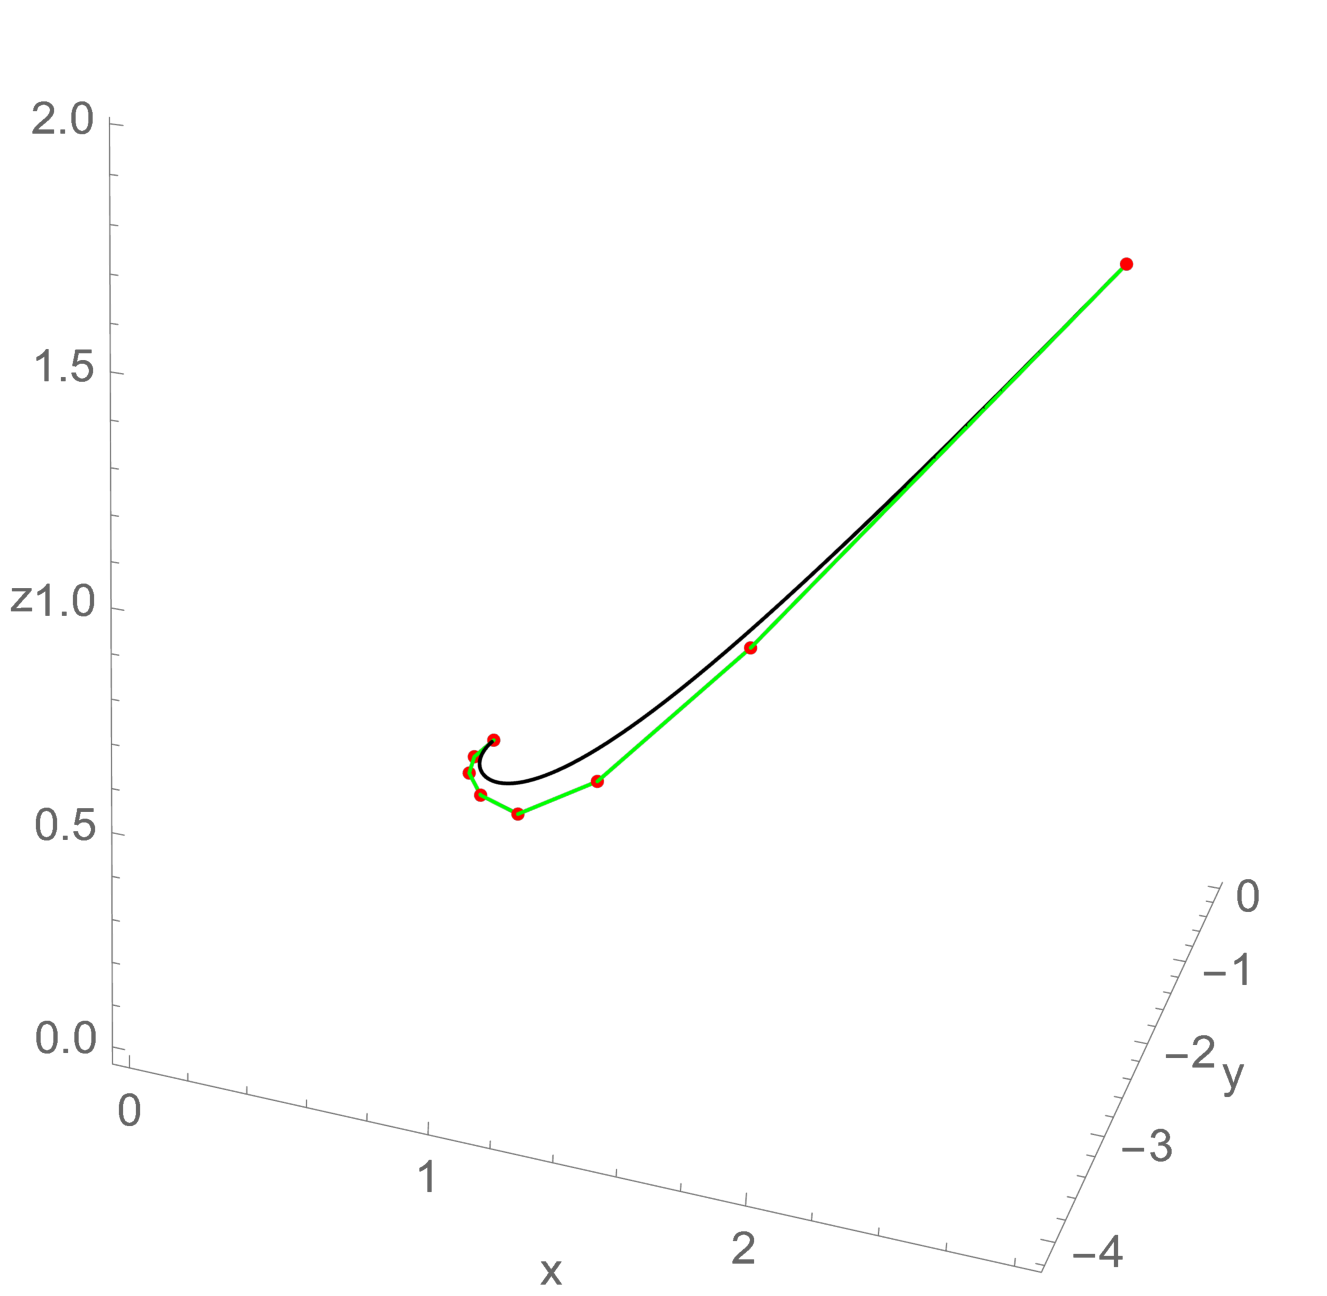
\includegraphics[width=0.5\textwidth]{images/h4w0_nevijacna.pdf}
	% \caption[caption za v kazalo]{Dolg caption pod sliko}
	  \caption[Primer nevijačne krivulje ($\st(h)=4,$ $\st(\wV)=0$)]{Na sliki je razviden graf vijačne krivulje s pripadajočim kontrolnim poligonom, za katero velja $\st(h)=4$ in $\st(\wV)=0.$}
	  \label{fig:h4w0_nevijacna}
	\end{figure}
	
	Kontrolne točke krivulje izračunamo preko enačb \eqref{kontrolne_tocke}. Enake so
	\begin{align*}
		\pV_0&=(0,0,0),&\pV_4&=(0.4, -1.07619, 0.0285714),\\
		\pV_1&=(0, -0.285714, 0),&\pV_5&=(0.819048, -1.55238, 0.257143),\\
		\pV_2&=(0.047619, -0.52381, 0)&\pV_6&=(1.53333, -2.45714, 0.828571),\\
		\pV_3&=(0.171429, -0.790476, 0)&\pV_7&=(2.81905, -4.17143, 1.97143).
	\end{align*}
	Tako dobimo krivuljo $\rV,$ ki ima komponente enake
	\begin{align*}
		x(t)&=\frac{2}{7}t^7-\frac{2}{3}t^6+\frac{6}{5}t^5+t^3+t^2,\\
		y(t)&=-\frac{4}{7}t^7+\frac{8}{3}t^6-\frac{28}{5}t^5+3t^4-\frac{8}{3}t^3+t^2-2t,\\
		z(t)&=\frac{4}{7}t^7-2t^6+\frac{12}{5}t^5+t^4.
	\end{align*}
	Hodograf je primitiven, saj velja $\gcd(x'(t),y'(t),z'(t))=1.$ Parametrična hitrost krivulje $\sigma(t)$ je enaka
	\begin{equation*}
		\sigma(t)=\lVert\rV'(t)\rVert=6t^6-20t^5+30t^4-8t^3+9t^2-2t+2.
	\end{equation*}
	Razmerje med fleksijsko in torzijsko ukrivljenostjo je enako
	\begin{equation*}
		\left|\frac{\kappa(t)}{\tau(t)}\right|=\left|\frac{-2t^4+4t^3-6t^2+4t+1}{8t^4+2t^3-6t^2+12t}\right|,
	\end{equation*}
	kar ni identično enako konstanti. Tudi po Lancretovem izreku \ref{lancret} lahko preverimo, da je taka krivulja nevijačna.
\end{primer}

%%%%%%%%%%%%%%%%%%%%%%%%%%%%%%%%%%%%%%%%%%%%%%%%%%%%%%%%%%%%%%%%%%%%



%\section{Integrali po \texorpdfstring{$\omega$}{ω}-kompleksih}
%\subsection{Definicija}
%\begin{definicija}
%  Neskončno zaporedje kompleksnih števil, označeno z $\omega = (\omega_1, \omega_2, \ldots)$,
%  se imenuje \emph{$\omega$-kompleks}.\footnote{To ime je izmišljeno.}
%
%  Črni blok zgoraj je tam namenoma. Označuje, da \LaTeX{} ni znal vrstice prelomiti pravilno
%  in vas na to opozarja. Preoblikujte stavek ali mu pomagajte deliti problematično besedo z
%  ukazom \verb|\hyphenation{an-ti-ko-mu-ta-ti-ven}| v preambuli.
%\end{definicija}
%\begin{trditev}[Znano ime ali avtor]
%  \label{trd:obstoj-omega}
%  Obstaja vsaj en $\omega$-kompleks.
%\end{trditev}
%\begin{proof}
%  Naštejmo nekaj primerov:
%  \begin{align}
%    \omega &= (0, 0, 0, \dots), \label{eq:zero-kompleks} \\
%    \omega &= (1, i, -1, -i, 1, \ldots), \nonumber \\
%    \omega &= (0, 1, 2, 3, \ldots). \nonumber \qedhere  % postavi QED na zadnjo vrstico enačbe
%  \end{align}
%\end{proof}
%
%\section{Tehnični napotki za pisanje}
%
%\subsection{Sklicevanje in citiranje}
%Za sklice uporabljamo \verb|\ref|, za sklice na enačbe \verb|\eqref|, za citate \verb|\cite|. Pri
%sklicevanju in citiranju sklicano številko povežemo s prejšnjo besedo z nedeljivim presledkom
%$\sim$, kot npr.\ \verb|iz trditve~\ref{trd:obstoj-omega} vidimo|.
%
%\begin{primer}
%  Zaporedje~\eqref{eq:zero-kompleks} iz dokaza trditve~\ref{trd:obstoj-omega} na
%  strani~\pageref{trd:obstoj-omega} lahko najdemo tudi v Spletni enciklopediji zaporedij~\cite{oeis}.
%  Citiramo lahko tudi bolj natančno~\cite[trditev 2.1, str.\ 23]{lebedev2009introduction}.
%\end{primer}
%
%\subsection{Okrajšave}
%Pri uporabi okrajšav \LaTeX{} za piko vstavi predolg presledek, kot npr. tukaj. Zato se za vsako
%piko, ki ni konec stavka doda presledek običajne širine z ukazom \verb*|\ |, kot npr.\ tukaj.
%Primerjaj z okrajšavo zgoraj za razliko.
%
%\subsection{Vstavljanje slik}
%Sliko vstavimo v plavajočem okolju \texttt{figure}. Plavajoča okolja \emph{plavajo} po tekstu, in
%jih lahko postavimo na vrh strani z opcijskim parametrom `\texttt{t}', na lokacijo, kjer je v kodi s
%`\texttt{h}', in če to ne deluje, potem pa lahko rečete \LaTeX u, da ga \emph{res} želite tukaj,
%kjer ste napisali, s `\texttt{h!}'. Lepo je da so vstavljene slike vektorske (recimo \texttt{.pdf}
%ali \texttt{.eps} ali \texttt{.svg}) ali pa \texttt{.png} visoke resolucije (več kot
%\unit[300]{dpi}).  Pod vsako sliko je napis in na vsako sliko se skličemo v besedilu. Primer
%vektorske slike je na sliki~\ref{fig:sample}. Vektorsko sliko prepoznate tako, da močno
%zoomate v sliko, in še vedno ostane gladka. Več informacij je na voljo na
%\url{https://en.wikibooks.org/wiki/LaTeX/Floats,_Figures_and_Captions}. Če so slike bitne, kot na
%primer slika~\ref{fig:image}, poskrbite, da so v dovolj visoki resoluciji.
%
%\begin{figure}[h]
%  \centering
%  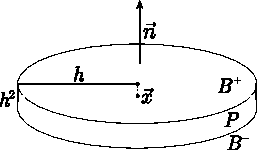
\includegraphics[width=0.6\textwidth]{images/sample.pdf}
%% \caption[caption za v kazalo]{Dolg caption pod sliko}
%  \caption[Primer vektorske slike.]{Primer vektorske slike z oznakami v enaki pisavi, kot jo
%     uporablja \LaTeX{}.  Narejena je s programom Inkscape, \LaTeX{} oznake so importane v
%     Inkscape iz pomožnega PDF.}
%  \label{fig:sample}
%\end{figure}
%
%\begin{figure}[h]
%  \centering
%  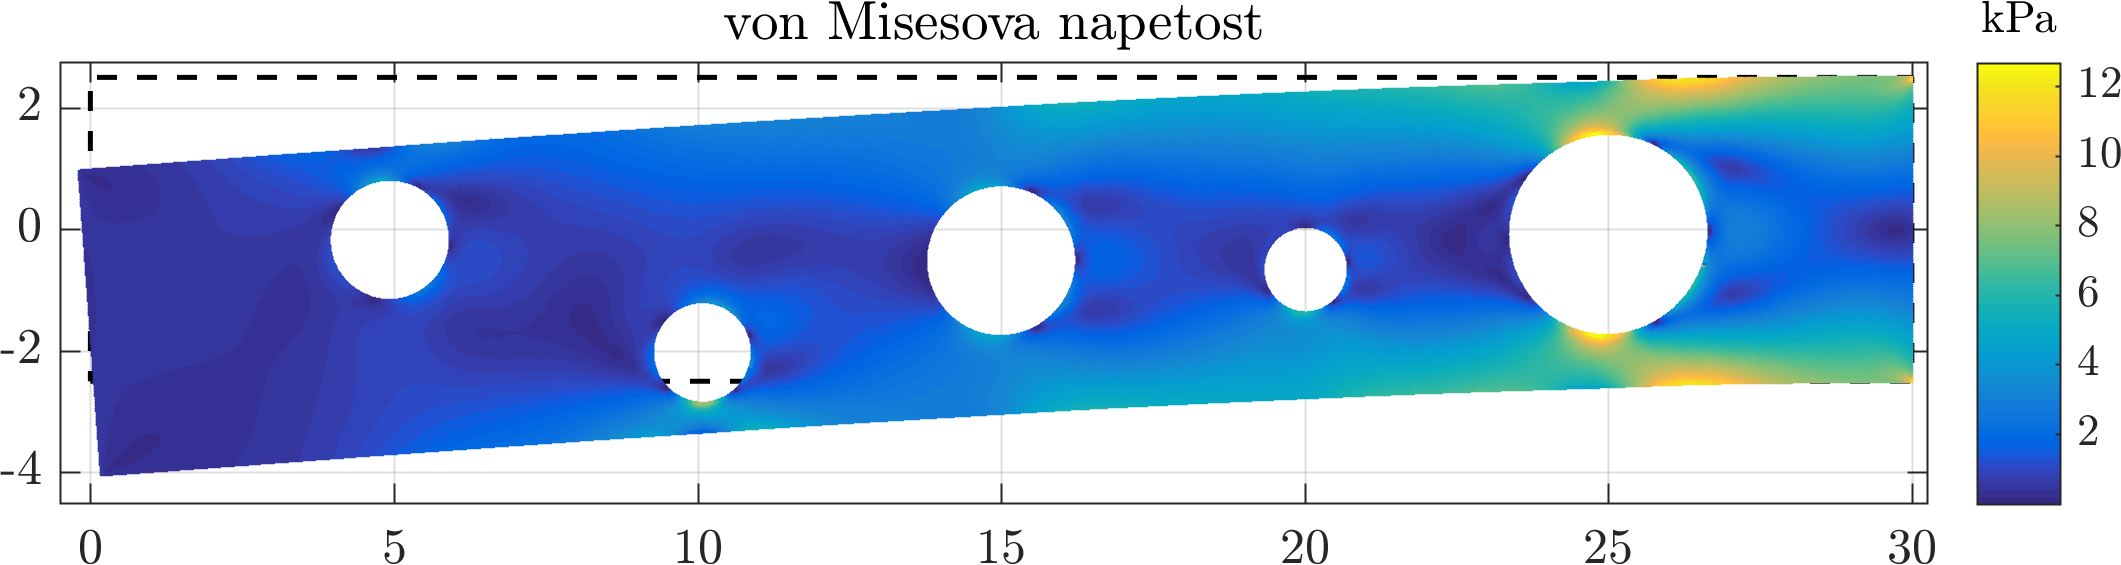
\includegraphics[width=0.8\textwidth]{images/image.png}
%  \caption[Primer bitne slike.]{Primer bitne slike, izvožene iz Matlaba. Poskrbite, da so slike v
%  dovolj visoki resoluciji in da ne vsebujejo prosojnih elementov (to zahteva PDF/A-1b format).}
%  \label{fig:image}
%\end{figure}
%
%\subsection{Kako narediti stvarno kazalo}
%Dodate ukaze \verb|\index{polje}| na besede, kjer je pojavijo, kot tukaj\index{tukaj}.
%Več o stvarnih kazalih je na voljo na \url{https://en.wikibooks.org/wiki/LaTeX/Indexing}.
%
%\subsection{Navajanje literature}
%%Članke citiramo z uporabo \verb|\cite{label}|, \verb|\cite[text]{label}| ali pa več naenkrat s
%%\verb|\cite\{label1, label2}|. Tudi tukaj predhodno besedo in citat povežemo z nedeljivim presledkom
%%$\sim$. Na primer~\cite{chen2006meshless,liu2001point}, ali pa \cite{kibriya2007empirical}, ali pa
%%\cite[str.\ 12]{trobec2015parallel}, \cite[enačba (2.3)]{pereira2016convergence}.
%%Vnosi iz \verb|.bib| datoteke, ki niso citirani, se ne prikažejo v seznamu literature, zato jih
%%tukaj citiram.~\cite{vene2000categorical}, \cite{gregoric2017stopniceni}, \cite{slak2015induktivni},
%%\cite{nsphere}, \cite{kearsley1975linearly}, \cite{STtemplate}, \cite{NunbergerTand}.
%
%Tu na novo citiram \cite{DPHclanek1}, \cite{DPHclanek2}, \cite{beltranmonterde}, \cite{choi2002clifford},
%\cite{struik1961lectures}, \cite{kreyszig2019differential}, \cite{faroukietal2004}, \cite{farouki2008pythagorean}. 

% Literatura:
% Primer navajanja na http://www.fmf.uni-lj.si/storage/24240/LiteraturaM.pdf,
% ampak bi moral stil poskrbeti za vse. Reference se uredijo po abecedi.
% Če nobena izbira izmed @book, @atricle,... ni ok, potem se lahko vse napiše v
% @misc pod note={} in deluje tako kot normalen LaTeX.
% Komentar v bib datoteki se naredi samo s parom { }
% Za urejanje literature avtor priporoča program Jabref, ki zna tudi avtomatsko
% okrajšati imena revij. Za pravilno sortiranje vnosov brez avtorja, uporabite
% polje key={ }, kot v primeru.
% V primeru napak ustvarite issue na GitHubu ali pišite na jure.slak@fmf.uni-lj.si.
\cleardoublepage                           % na desni strani
\phantomsection                            % da prav delujejo hiperlinki
\addcontentsline{toc}{section}{\bibname}   % dodajmo v kazalo
\bibliographystyle{fmf-sl}                 % uporabljen stil je v datoteki fmf-sl.bst, na voljo tudi angleška verzija
\bibliography{literatura.bib}                 % literatura je v datoteki, definirani na začetku
% TeXStudio zmede \ zgoraj, tako da lahko notri napišeš dejansko ime .bib datoteke, če ti
% ne delajo predlogi citatov.

% Za stvarno kazalo
\cleardoublepage                           % na desni strani
\phantomsection                            % da prav delujejo hiperlinki
\addcontentsline{toc}{section}{\indexname} % dodajmo v kazalo
\printindex

\end{document}
